% ─── Publication panel captions ───────────────────────────────────────────────
% Each figure* spans both columns.  Include this file with % ─── Publication panel captions ───────────────────────────────────────────────
% Each figure* spans both columns.  Include this file with % ─── Publication panel captions ───────────────────────────────────────────────
% Each figure* spans both columns.  Include this file with % ─── Publication panel captions ───────────────────────────────────────────────
% Each figure* spans both columns.  Include this file with \input{panels/events-captions}
% after the figures are placed in the manuscript.

% ──────────────────────────────────────────────────────────────────────────────
\begin{figure*}[!htbp]
    \centering
    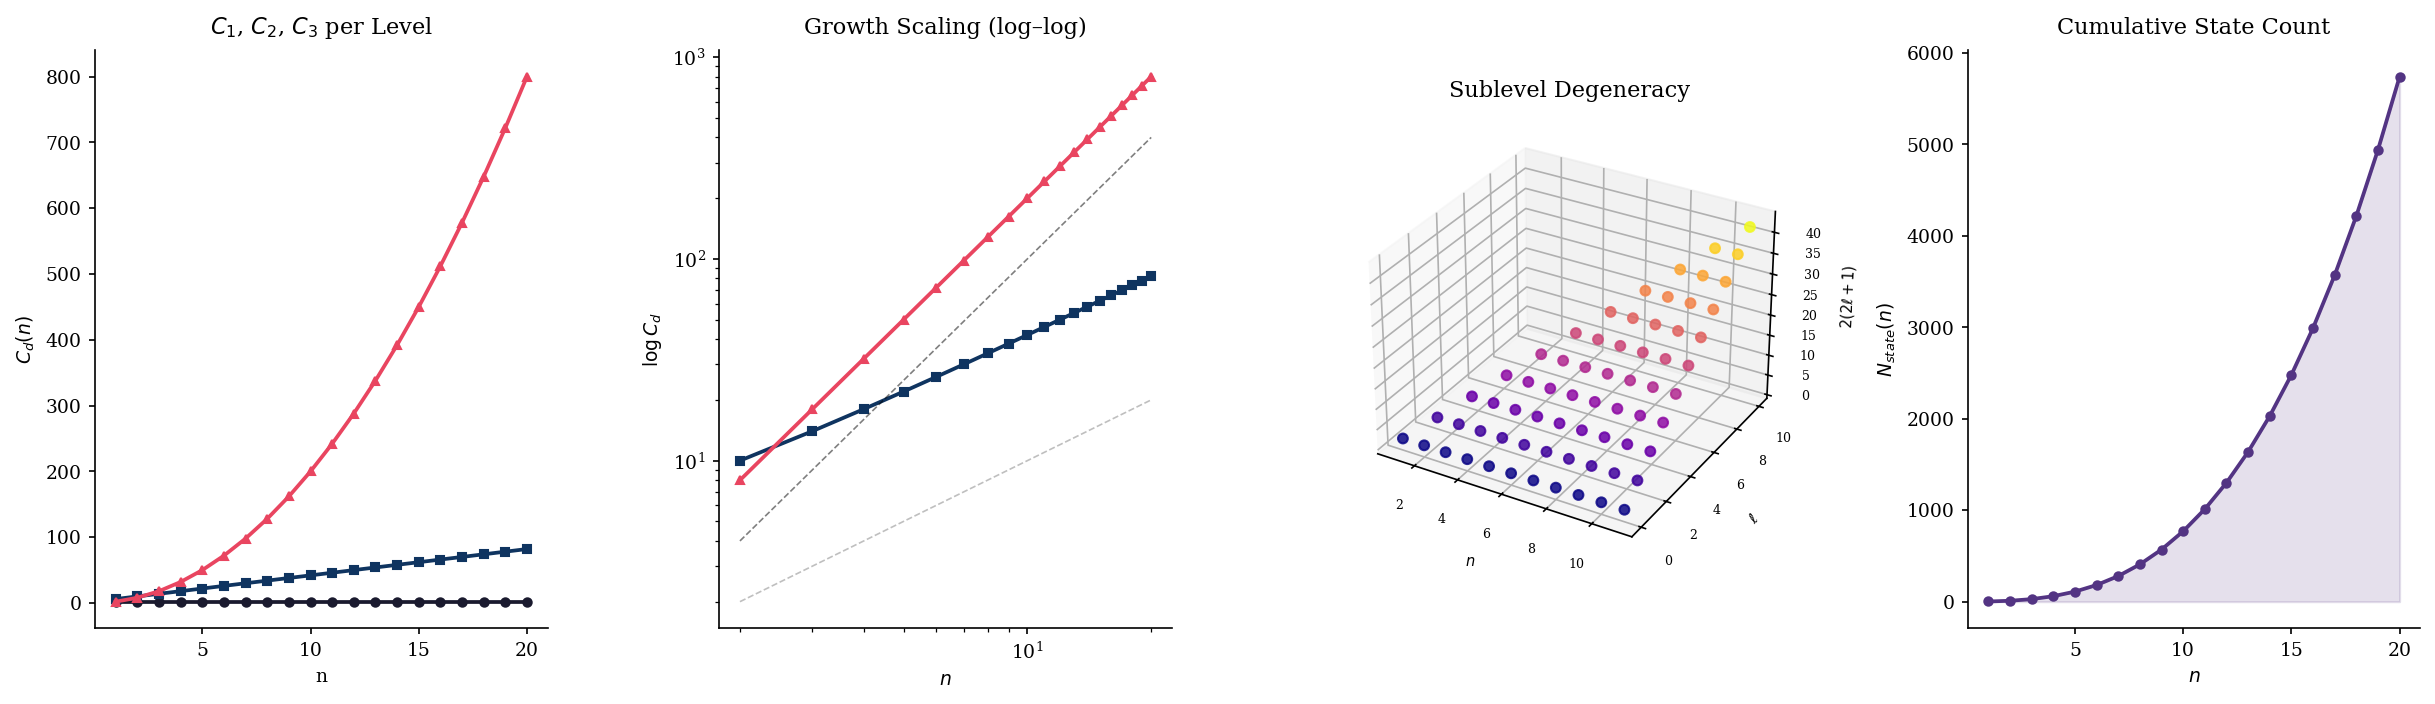
\includegraphics[width=\textwidth]{panels/panel_01_capacity_hierarchy.png}
    \caption{\textbf{Capacity growth $C_d(n)$ is constant in $d{=}1$, linear in $d{=}2$, and
    quadratic in $d{=}3$, establishing a strict dimensional hierarchy whose slope on a
    log–log axis discriminates the angular dimension of each within-level partition space
    (Definition~\ref{def:cap-d}; Theorem~\ref{thm:capacity}).}
    (\textbf{A})~Line plot of per-level capacity $C_d(n)$ versus principal quantum number $n$
    for $d{=}1$ (dark, flat), $d{=}2$ (mid, linear), and $d{=}3$ (light, quadratic).
    The three curves separate immediately at $n{=}2$: $C_1$ remains fixed at $2$; $C_2$
    grows as $4n{+}2$; $C_3 = 2n^2$ accelerates away from both, reflecting the
    two-dimensional angular structure of the within-level space $L_n^{(3)}$.
    (\textbf{B})~Log–log plot of $C_2(n)$ and $C_3(n)$ for $n \geq 3$, overlaid with reference
    lines of slope $1$ (linear, grey dashed) and slope $2$ (quadratic, black dashed).
    $C_2$ tracks the slope-$1$ reference exactly; $C_3$ tracks slope $2$ exactly,
    confirming that the exponent of capacity growth equals the continuous angular
    dimension of $L_n^{(d)}$: $0$ for $d{=}1$, $1$ for $d{=}2$, $2$ for $d{=}3$.
    (\textbf{C})~Three-dimensional scatter of sublevel degeneracy $2(2\ell+1)$ plotted against
    principal level $n$ (x-axis) and angular index $\ell$ (y-axis) for $n = 1,\ldots,11$.
    Colour encodes degeneracy magnitude (plasma scale).  The surface rises along both
    axes, with the steepest growth in $\ell$ at fixed $n$, reproducing the quadratic
    capacity as $C_3(n) = \sum_{\ell=0}^{n-1} 2(2\ell{+}1)$.
    (\textbf{D})~Line plot of cumulative state count $N_\mathrm{state}(n) = n(n{+}1)(2n{+}1)/3$
    versus $n$ with shaded fill.  The cubic growth follows directly from summing the
    quadratic per-level capacity; the steepening curvature is the algebraic signature
    that each added level contributes an accelerating number of partition states, as
    stated in Corollary~\ref{cor:cumulative}.}%
    \label{fig:panel1_capacity_hierarchy}
\end{figure*}

% ──────────────────────────────────────────────────────────────────────────────
\begin{figure*}[!htbp]
    \centering
    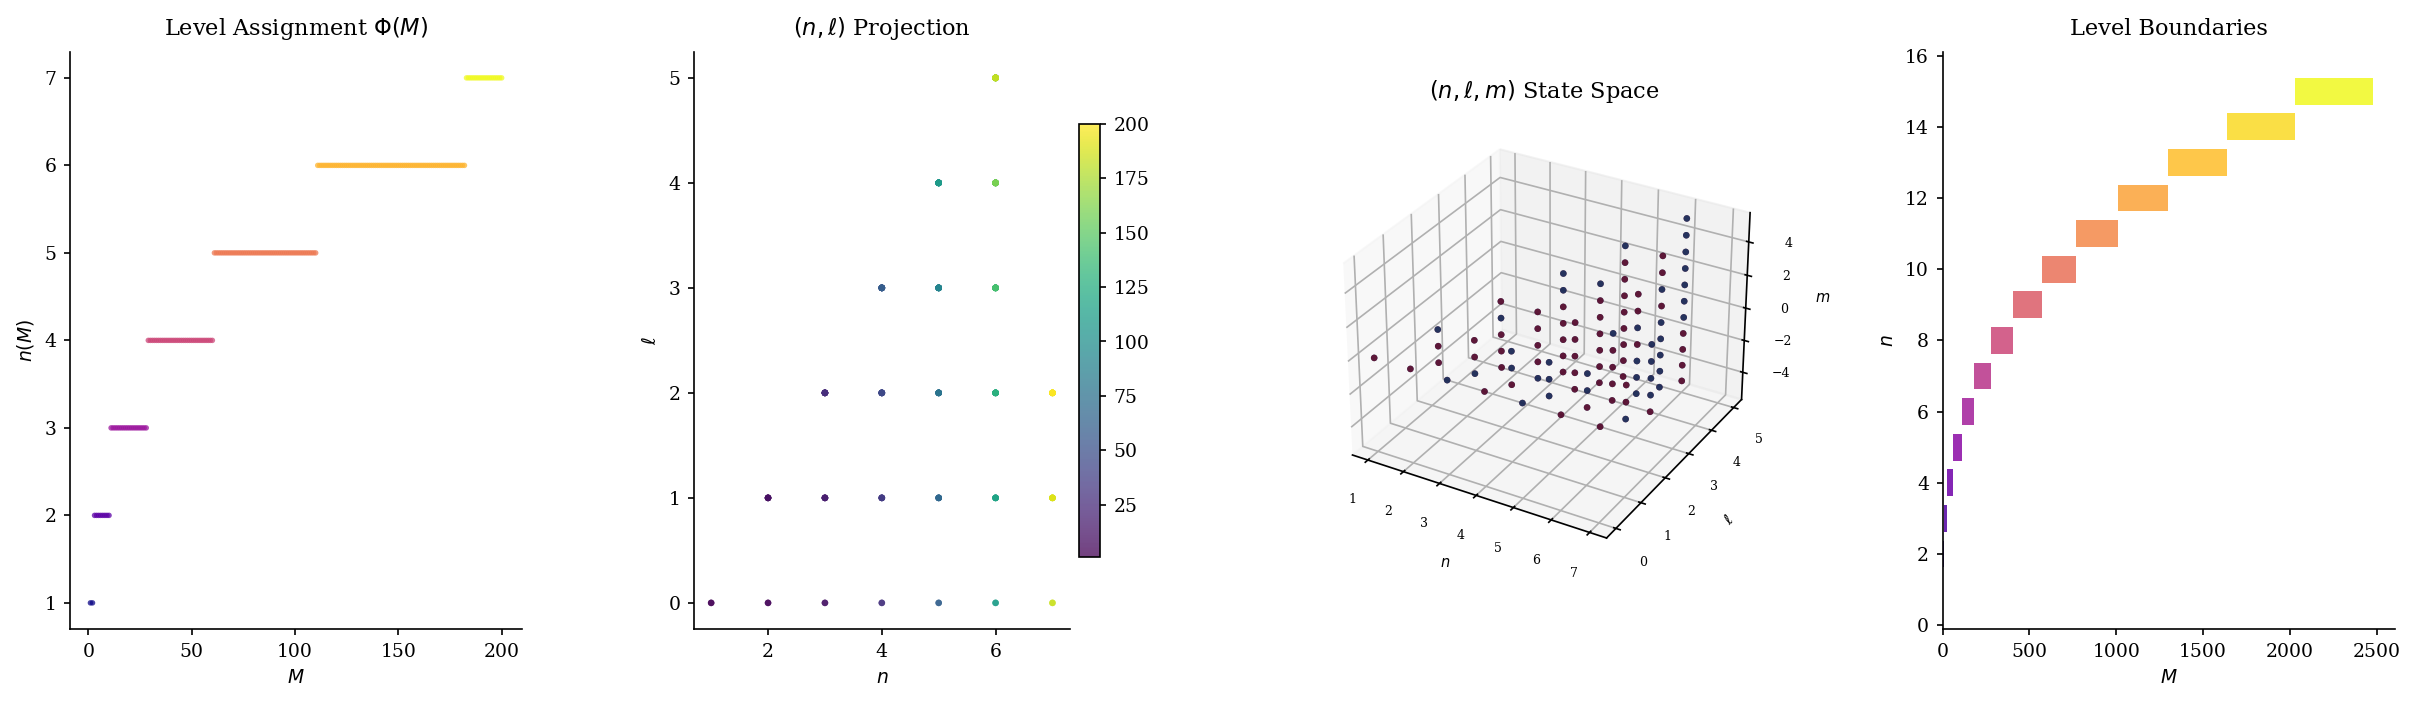
\includegraphics[width=\textwidth]{panels/panel_02_bijection_structure.png}
    \caption{\textbf{The partition map $\Phi:\mathbb{Z}^{+}\!\to\mathcal{P}$ is a
    well-defined bijection whose image tiles three-dimensional quantum-number space
    without collision or gap, and whose level boundaries are sharp staircase
    transitions determined by the cumulative capacity formula
    (Theorem~\ref{thm:bijection}; Corollary~\ref{cor:cumulative}).}
    (\textbf{A})~Scatter of principal level $n(\Phi(M))$ versus integer index $M$ for
    $M = 1,\ldots,200$, coloured by $n$ (plasma scale).  Level transitions appear as
    discrete upward steps; within each band $M$ increments uniformly, confirming
    that $\Phi$ exhausts every state of level $n$ before advancing to $n{+}1$.
    (\textbf{B})~Two-dimensional projection onto the $(n,\ell)$ plane, coloured by $M$
    (viridis scale).  Each point $(n,\ell)$ appears with multiplicity $2(2\ell{+}1)$,
    one for each $(m,s)$ pair; the colour gradient shows that $M$ increases
    monotonically left-to-right and bottom-to-top within each level, establishing
    the lexicographic ordering of $\Phi$.
    (\textbf{C})~Three-dimensional scatter of the full quantum-number triple $(n,\ell,m)$
    for $M = 1,\ldots,200$, with colour encoding spin $s = \pm\tfrac{1}{2}$ (red–blue
    diverging scale).  The cloud fills a triangular prism in $(n,\ell,m)$ space:
    $0 \leq \ell \leq n{-}1$, $-\ell \leq m \leq \ell$.  No two points coincide,
    providing visual confirmation of injectivity (Theorem~\ref{thm:bijection}).
    (\textbf{D})~Horizontal bar chart of level sizes: each bar spans the $M$-range
    $[N_\mathrm{state}(n{-}1){+}1,\, N_\mathrm{state}(n)]$ for levels $n = 1,\ldots,15$,
    coloured by level index.  Bar widths equal $C_3(n) = 2n^2$, growing quadratically;
    the staircase of left boundaries locates the exact $M$-index at which each new
    principal level begins, as derived in Corollary~\ref{cor:cumulative}.}%
    \label{fig:panel2_bijection_structure}
\end{figure*}

% ──────────────────────────────────────────────────────────────────────────────
\begin{figure*}[!htbp]
    \centering
    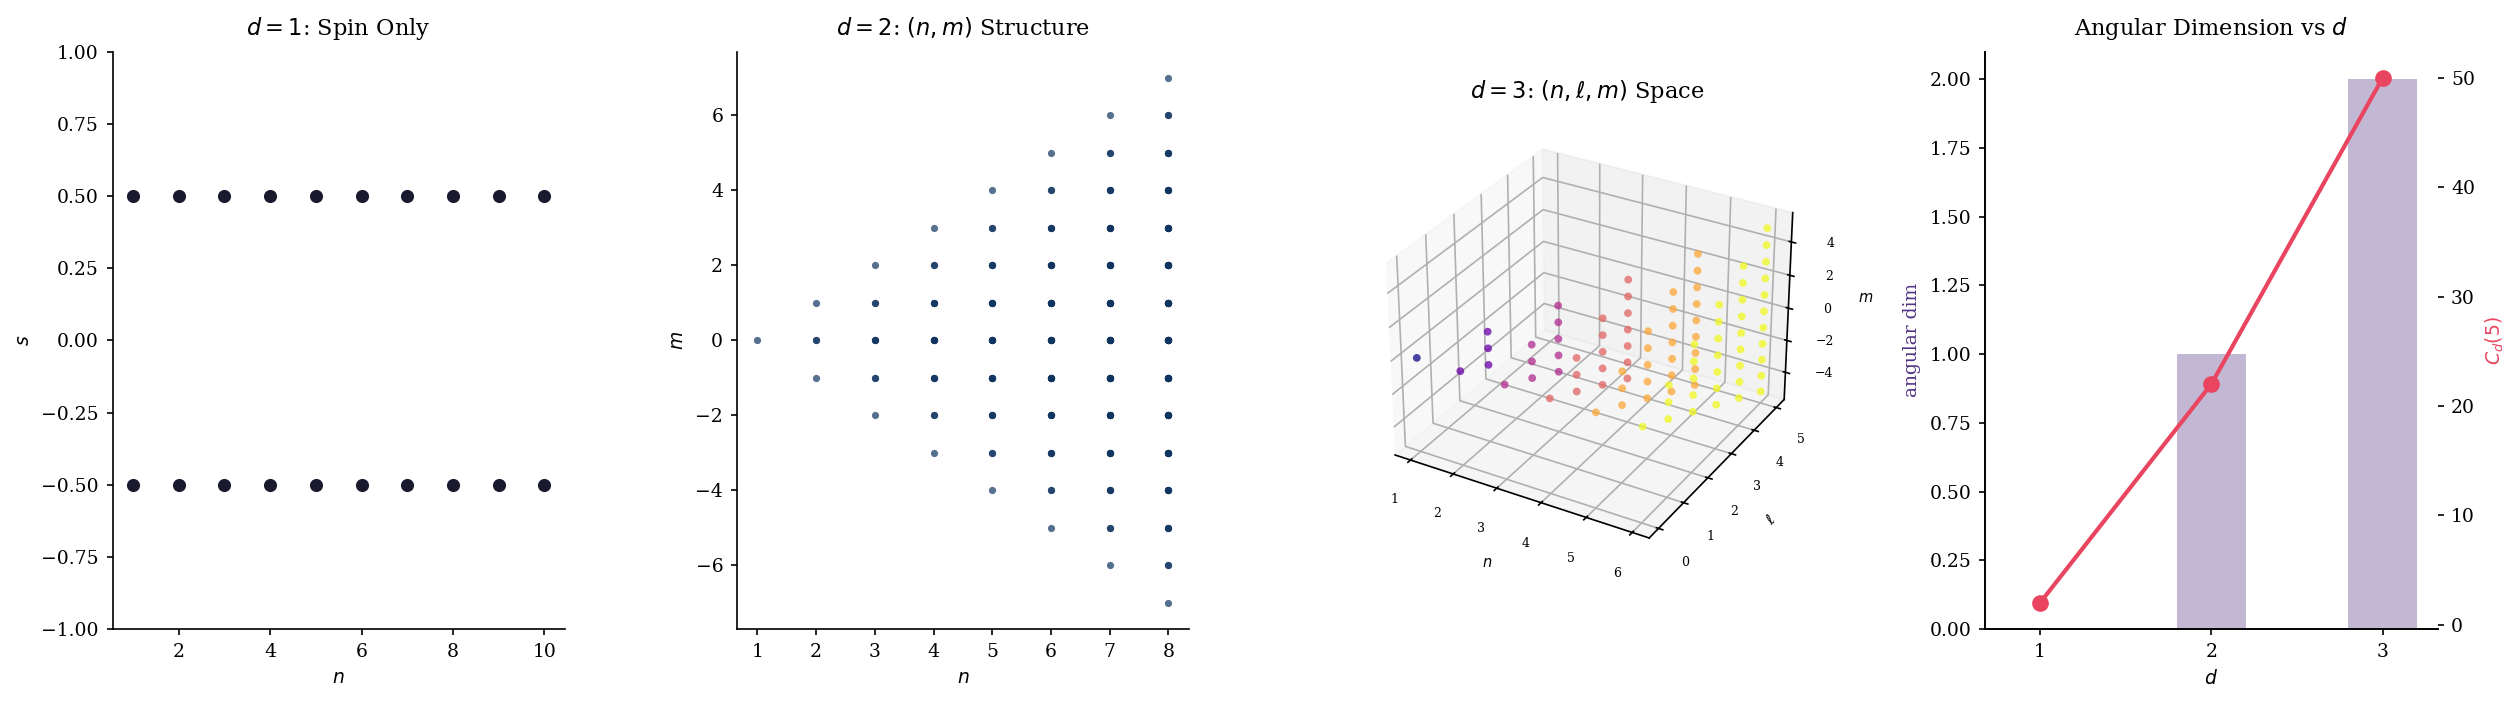
\includegraphics[width=\textwidth]{panels/panel_03_partition_geometry.png}
    \caption{\textbf{Spatial dimension $d{=}3$ is the minimum for which the within-level
    partition space $L_n^{(d)}$ has continuous angular dimension $\geq 2$, enabling
    negation to close around any state from all angular directions simultaneously
    (Theorem~\ref{thm:min-dim}; Definition~\ref{def:within-level}).}
    (\textbf{A})~Scatter of partition states in $d{=}1$: only the spin coordinate $s =
    \pm\tfrac{1}{2}$ varies; every level $n$ contributes exactly two isolated points.
    The within-level space $L_n^{(1)}$ has angular dimension $0$: there is no
    continuous angular degree of freedom, so negation from the ``left'' and ``right''
    cannot simultaneously enclose the state.
    (\textbf{B})~Scatter of partition states $(n, m)$ for $d{=}2$, $n = 1,\ldots,8$.
    Within level $n$, the $m$-values $\{-(n{-}1),\ldots,n{-}1\}$ form a one-dimensional
    chain; $L_n^{(2)}$ has angular dimension $1$.  Two opposing states can bracket any
    given $m$, but the within-level topology is a line segment, not a closed surface,
    so negation-closure is incomplete.
    (\textbf{C})~Three-dimensional scatter of partition states $(n, \ell, m)$ for $d{=}3$,
    $n = 1,\ldots,6$, coloured by $n$ (plasma scale).  Within level $n$, the pairs
    $(\ell, m)$ fill a two-dimensional triangular region; $L_n^{(3)}$ has angular
    dimension $2$.  Every interior point is enclosed from all angular directions,
    satisfying the closure condition of Theorem~\ref{thm:min-dim}.
    (\textbf{D})~Combined bar and line chart comparing angular dimension (left axis, bars)
    and per-level capacity $C_d(5)$ (right axis, line with markers) for $d = 1, 2, 3$.
    Angular dimension steps $0 \to 1 \to 2$ in exact correspondence with the
    exponent governing $C_d$, confirming that the quadratic capacity of $d{=}3$ is the
    algebraic signature of the minimum dimensionality required for
    negation-constituted closure.}%
    \label{fig:panel3_partition_geometry}
\end{figure*}

% ──────────────────────────────────────────────────────────────────────────────
\begin{figure*}[!htbp]
    \centering
    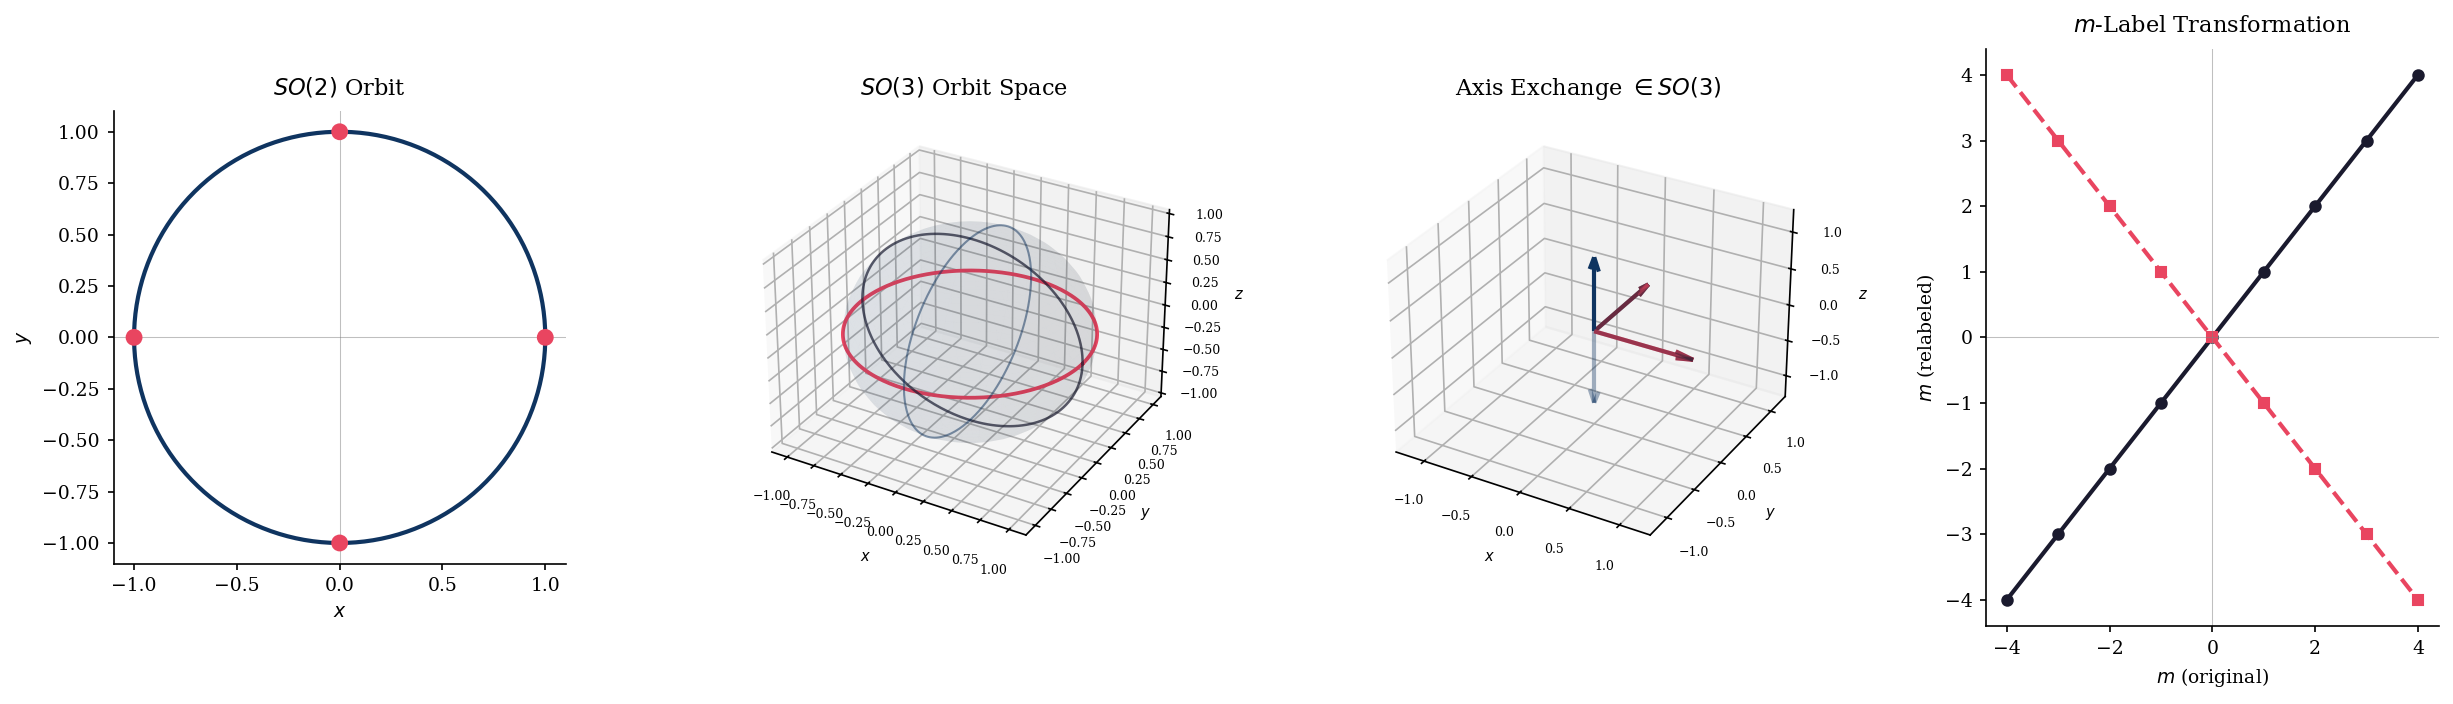
\includegraphics[width=\textwidth]{panels/panel_04_SO3_symmetry.png}
    \caption{\textbf{The axis exchange $(x,y,z)\mapsto(y,x,-z)$ is a proper rotation
    in $SO(3)$ with $\det = +1$, but the analogous swap $x \leftrightarrow y$ in
    $d{=}2$ is an improper reflection with $\det = -1$; consequently, the
    $m$-label is $SO(2)$-invariant but changes under $SO(3)$ axis relabelling,
    and partition identity is reference-frame-independent only for $d\geq 3$
    (Corollary~\ref{cor:axis-exchange}).}
    (\textbf{A})~$SO(2)$ orbit: unit circle in the $xy$-plane with four marked points at
    $(\pm 1, 0)$ and $(0, \pm 1)$.  All rotations in $SO(2)$ preserve orientation;
    the swap $x \leftrightarrow y$ in two dimensions corresponds to reflection
    across the diagonal, an element of $O(2) \setminus SO(2)$ with $\det = -1$.
    (\textbf{B})~$SO(3)$ orbit space: transparent unit sphere with equatorial orbit
    (coloured ring, equator plane) and two meridional great-circle orbits.  The full
    $SO(3)$ orbit of a fixed axis direction sweeps a two-sphere, capturing the
    additional degree of freedom absent in $d{=}2$.
    (\textbf{C})~Three-dimensional axis-frame diagram visualising the exchange
    $R: (x,y,z)\mapsto(y,x,-z)$.  Solid arrows show the original frame
    $(\hat{e}_x, \hat{e}_y, \hat{e}_z)$; translucent arrows show the relabelled
    frame.  This transformation lies in $SO(3)$ ($\det R = +1$, angle $=\pi$ about
    the axis $\frac{1}{\sqrt{2}}(\hat{e}_x + \hat{e}_y)$), making it a physically
    accessible change of reference frame rather than an orientation reversal.
    (\textbf{D})~Line plot of the $m$-label transformation for $\ell = 4$ under the two
    symmetry groups.  Under $SO(2)$ rotation about $\hat{z}$, the eigenvalue $m$
    is invariant (identity line, dark).  Under the $SO(3)$ axis exchange of panel
    (C), $L_z \to -L_z$ and $m \mapsto -m$ (reflected line, light).  The
    non-trivial relabelling confirms that $m$ encodes a reference-frame choice,
    not an observer-independent integer, whenever $d \geq 3$.}%
    \label{fig:panel4_SO3_symmetry}
\end{figure*}

% ──────────────────────────────────────────────────────────────────────────────
\begin{figure*}[!htbp]
    \centering
    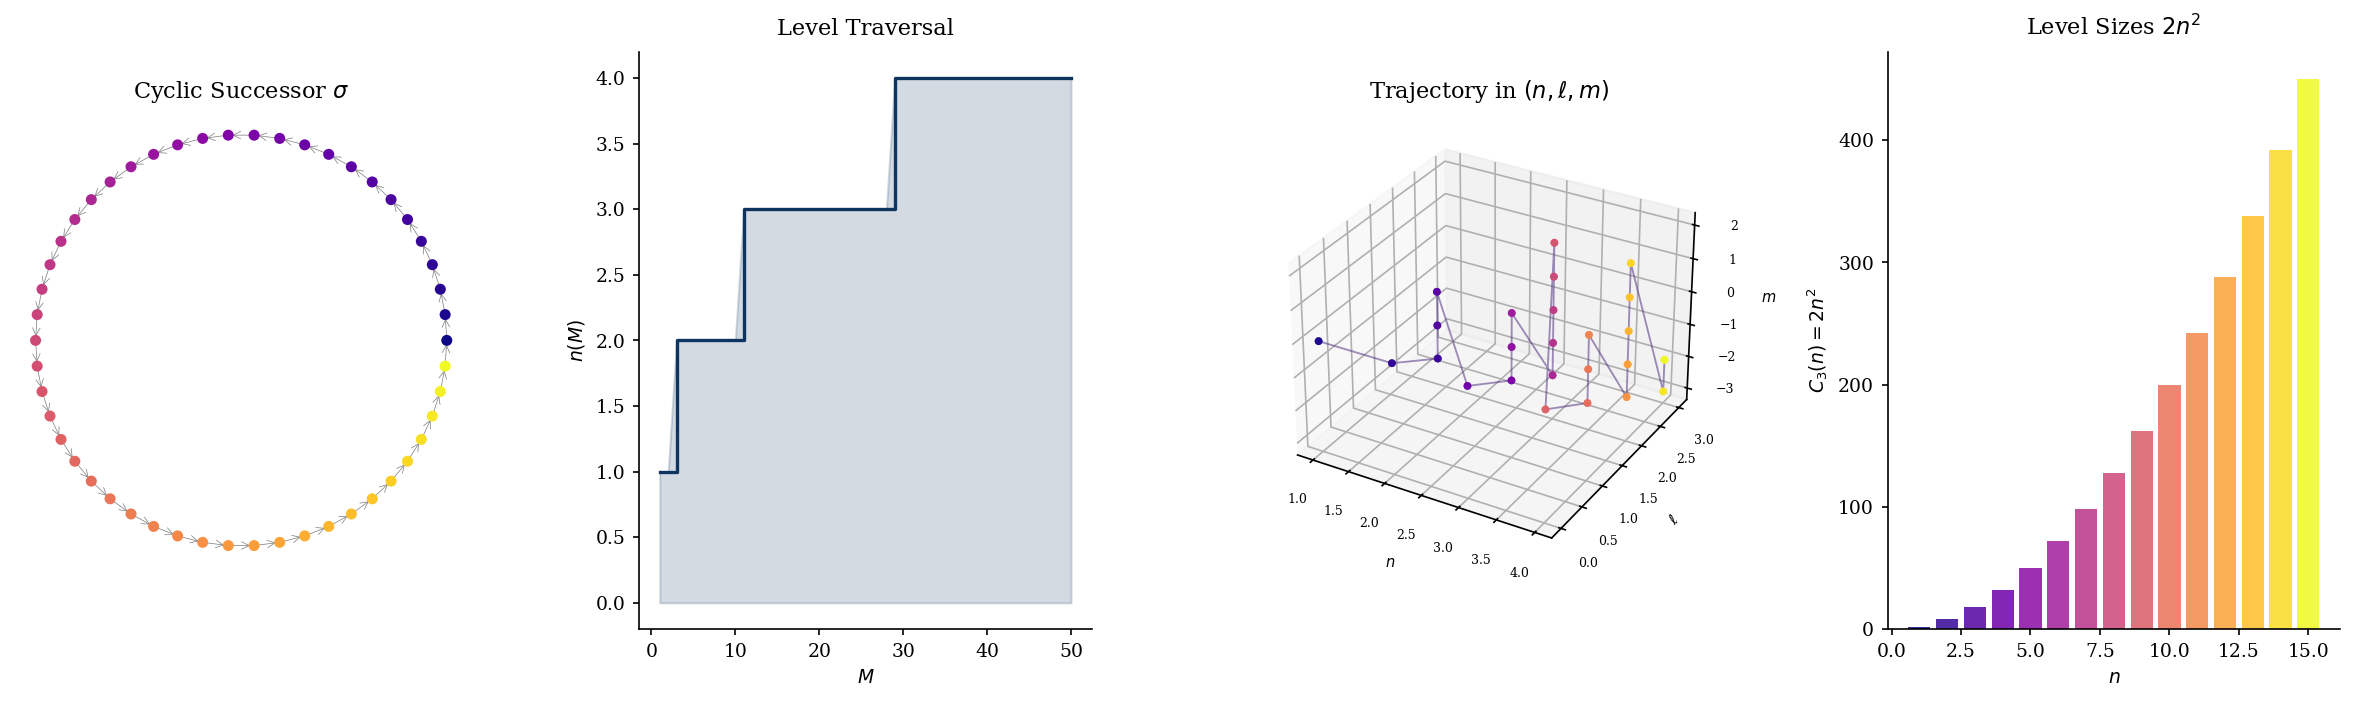
\includegraphics[width=\textwidth]{panels/panel_05_cyclic_closure.png}
    \caption{\textbf{The successor relation $\sigma$ is a bijection on the finite partition
    category $\mathcal{C}$ whose unique cycle has length $M_{\max} = N_\mathrm{state}(n_{\max})$,
    forcing every state—including $\Phi(1)$—to be revisited exactly once per period and
    making cyclic closure a structural consequence of finiteness rather than a dynamical
    assumption (Theorem~\ref{thm:cyclic}; Theorem~\ref{thm:cat-closure}).}
    (\textbf{A})~Cyclic successor diagram for $M_{\max} = 50$: each partition state is
    placed on a unit circle at angle $2\pi M / M_{\max}$, coloured by $M$ (plasma
    scale), with grey arrows connecting $\Phi(M)$ to $\sigma(\Phi(M)) = \Phi(M{+}1)$.
    The final arrow from $\Phi(50)$ returns to $\Phi(1)$, completing the cycle and
    confirming that $\sigma$ is a permutation of $\mathcal{C}$ with no fixed points
    and no proper sub-cycles (Theorem~\ref{thm:cyclic}).
    (\textbf{B})~Step plot of the level assignment $n(M)$ for $M = 1,\ldots,50$, with
    shaded fill below the curve.  Each plateau spans exactly $C_3(n) = 2n^2$ consecutive
    integers; the risers are instantaneous, reflecting the sharp level boundary at
    $M = N_\mathrm{state}(n)$.  The sequence is strictly non-decreasing (Theorem~\ref{thm:monotone}),
    encoding the irreversibility of temporal progression within the bijective ordering.
    (\textbf{C})~Three-dimensional trajectory through $(n, \ell, m)$ state space for
    $M = 1,\ldots,50$, with points coloured by $M$ (plasma scale) and connected by a
    curve.  The path climbs through successive levels, executes a zig-zag pattern
    within each level as $\ell$ and $m$ increment lexicographically, then returns to
    the origin upon cyclic closure.  The trajectory is injective on any open arc but
    closed as a whole (Corollary~\ref{cor:cyclic}).
    (\textbf{D})~Bar chart of level sizes $C_3(n) = 2n^2$ for $n = 1,\ldots,15$, coloured
    by level index.  Quadratic growth of bar height reflects the quadratic capacity law;
    the total area equals $M_{\max} = N_\mathrm{state}(n_{\max})$, the unique cycle length.
    The accelerating size of successive levels means that higher-$n$ states are
    structurally ``harder to reach'' in the sense of requiring a longer prefix of
    the successor sequence.}%
    \label{fig:panel5_cyclic_closure}
\end{figure*}

% ──────────────────────────────────────────────────────────────────────────────
\begin{figure*}[!htbp]
    \centering
    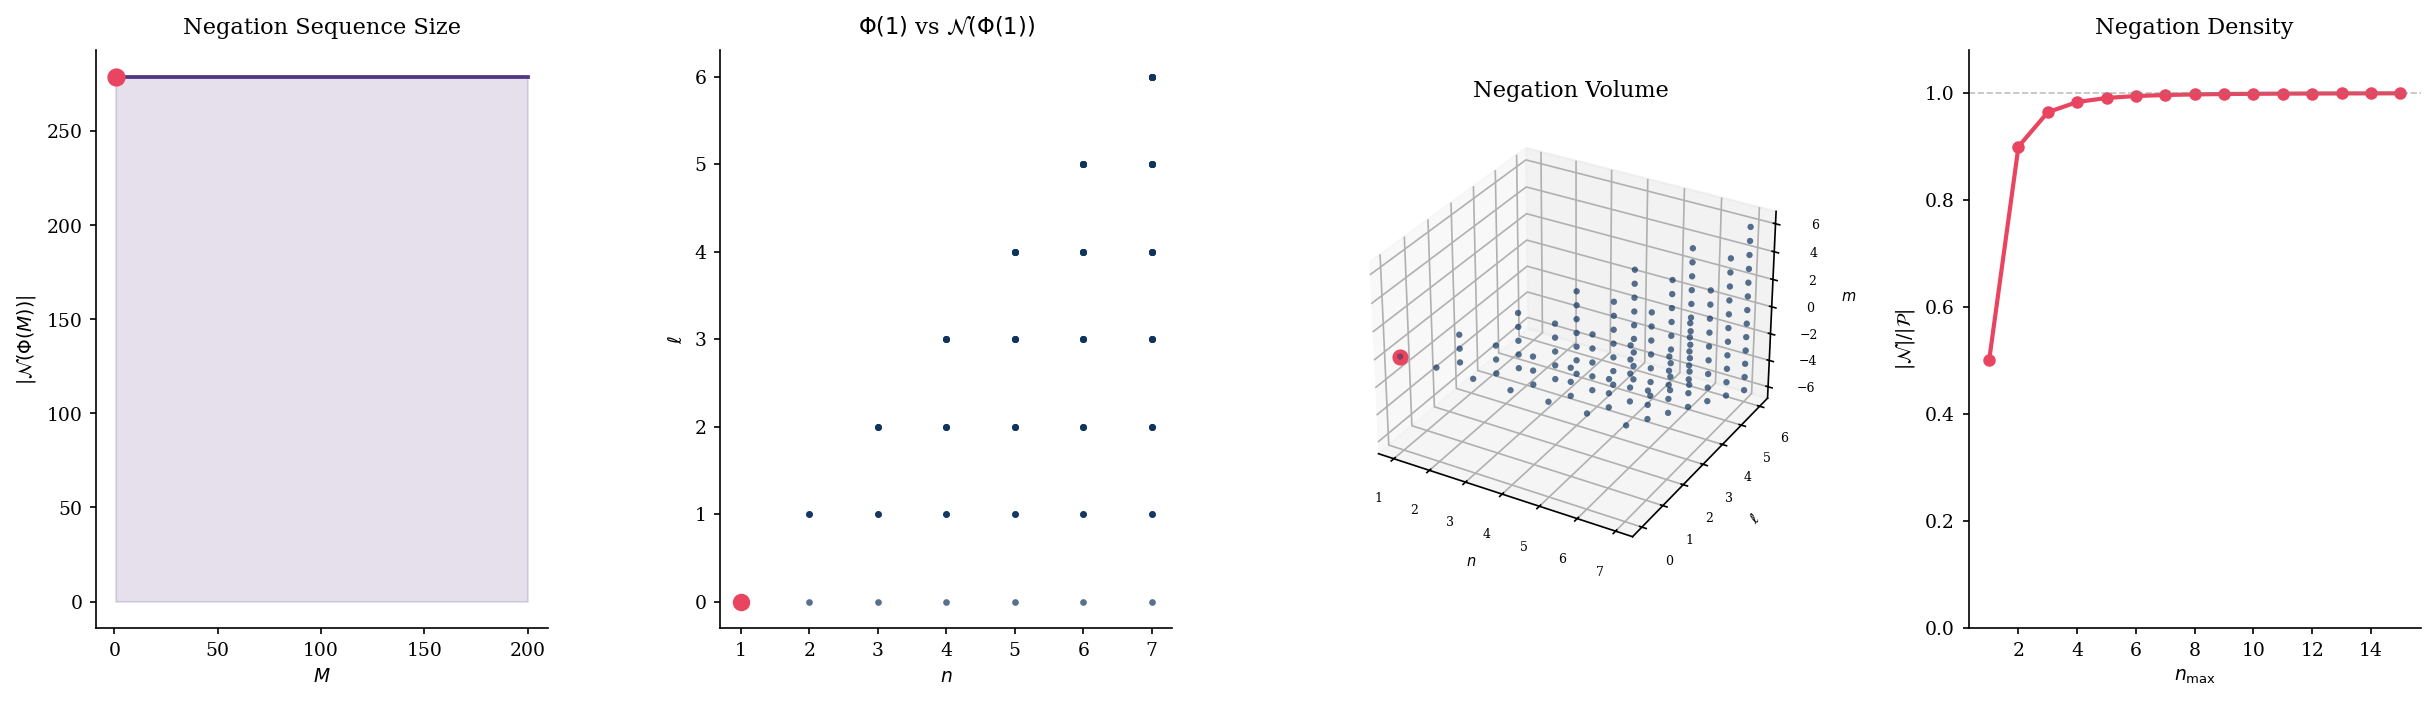
\includegraphics[width=\textwidth]{panels/panel_06_negation_identity.png}
    \caption{\textbf{Every partition state $\Phi(M)$ is uniquely identified by its negation
    sequence $\mathcal{N}(\Phi(M)) = \mathcal{P} \setminus \{\Phi(M)\}$, and the ground
    state $\Phi(1) = (1,0,0,+\tfrac{1}{2})$ possesses the largest possible negation
    sequence while being categorically irreducible, making it the structurally necessary
    origin of the partition sequence
    (Theorem~\ref{thm:negation-duality}; Definition~\ref{def:ground-cat};
    Theorem~\ref{thm:sing-necessity}).}
    (\textbf{A})~Scatter and fill of $|\mathcal{N}(\Phi(M))| = |\mathcal{P}| - 1$ versus $M$
    for $M = 1,\ldots,200$.  The value is constant across all $M$: every state has
    exactly one fewer element in its negation sequence than the cardinality of
    $\mathcal{P}$, because negation excludes only $\Phi(M)$ itself.  The ground state
    $\Phi(1)$ is marked (orange dot); it is distinguished not by a different negation
    size but by the property that $\Phi(1)$ has no $\sigma$-predecessor in
    $\mathcal{P}$ (Theorem~\ref{thm:sing-necessity}).
    (\textbf{B})~Two-dimensional scatter of the full partition space projected onto
    $(n, \ell)$ for $n = 1,\ldots,7$.  All states except $\Phi(1) = (1,0,0,+\tfrac{1}{2})$
    are shown in blue (the negation sequence $\mathcal{N}(\Phi(1))$); $\Phi(1)$ is marked
    in orange.  The visual contrast makes precise the duality $\mathcal{P} =
    \{\Phi(1)\} \cup \mathcal{N}(\Phi(1))$: identity is constituted by the totality
    of what it is not (Theorem~\ref{thm:negation-duality}).
    (\textbf{C})~Three-dimensional scatter of the full partition space in $(n, \ell, m)$
    for $n = 1,\ldots,7$.  Blue points form the negation volume $\mathcal{N}(\Phi(1))$;
    the single orange point at the origin $(1,0,0)$ is the ground state $\Phi(1)$.
    The geometric relationship captures the categorical claim: $\Phi(1)$ is the unique
    state maximally enclosed by its own negation set from all angular directions in
    the three-dimensional partition space.
    (\textbf{D})~Line plot of the negation density ratio $|\mathcal{N}| / |\mathcal{P}_{n_{\max}}|$
    versus the truncation level $n_{\max}$, where $|\mathcal{P}_{n_{\max}}| =
    N_\mathrm{state}(n_{\max})$.  The ratio $(N - 1)/N$ increases monotonically toward $1$
    as $n_{\max} \to \infty$, with the horizontal dashed line marking the asymptotic
    limit.  This convergence is the quantitative expression of the remark that any
    finite physical category saturates the negation relation: as the category grows,
    a state's identity becomes more fully determined by what it is not, with the
    ground state $\Phi(1)$ retaining the maximum negation complement at every
    finite truncation.}%
    \label{fig:panel6_negation_identity}
\end{figure*}

% ──────────────────────────────────────────────────────────────────────────────
\begin{figure*}[!htbp]
    \centering
    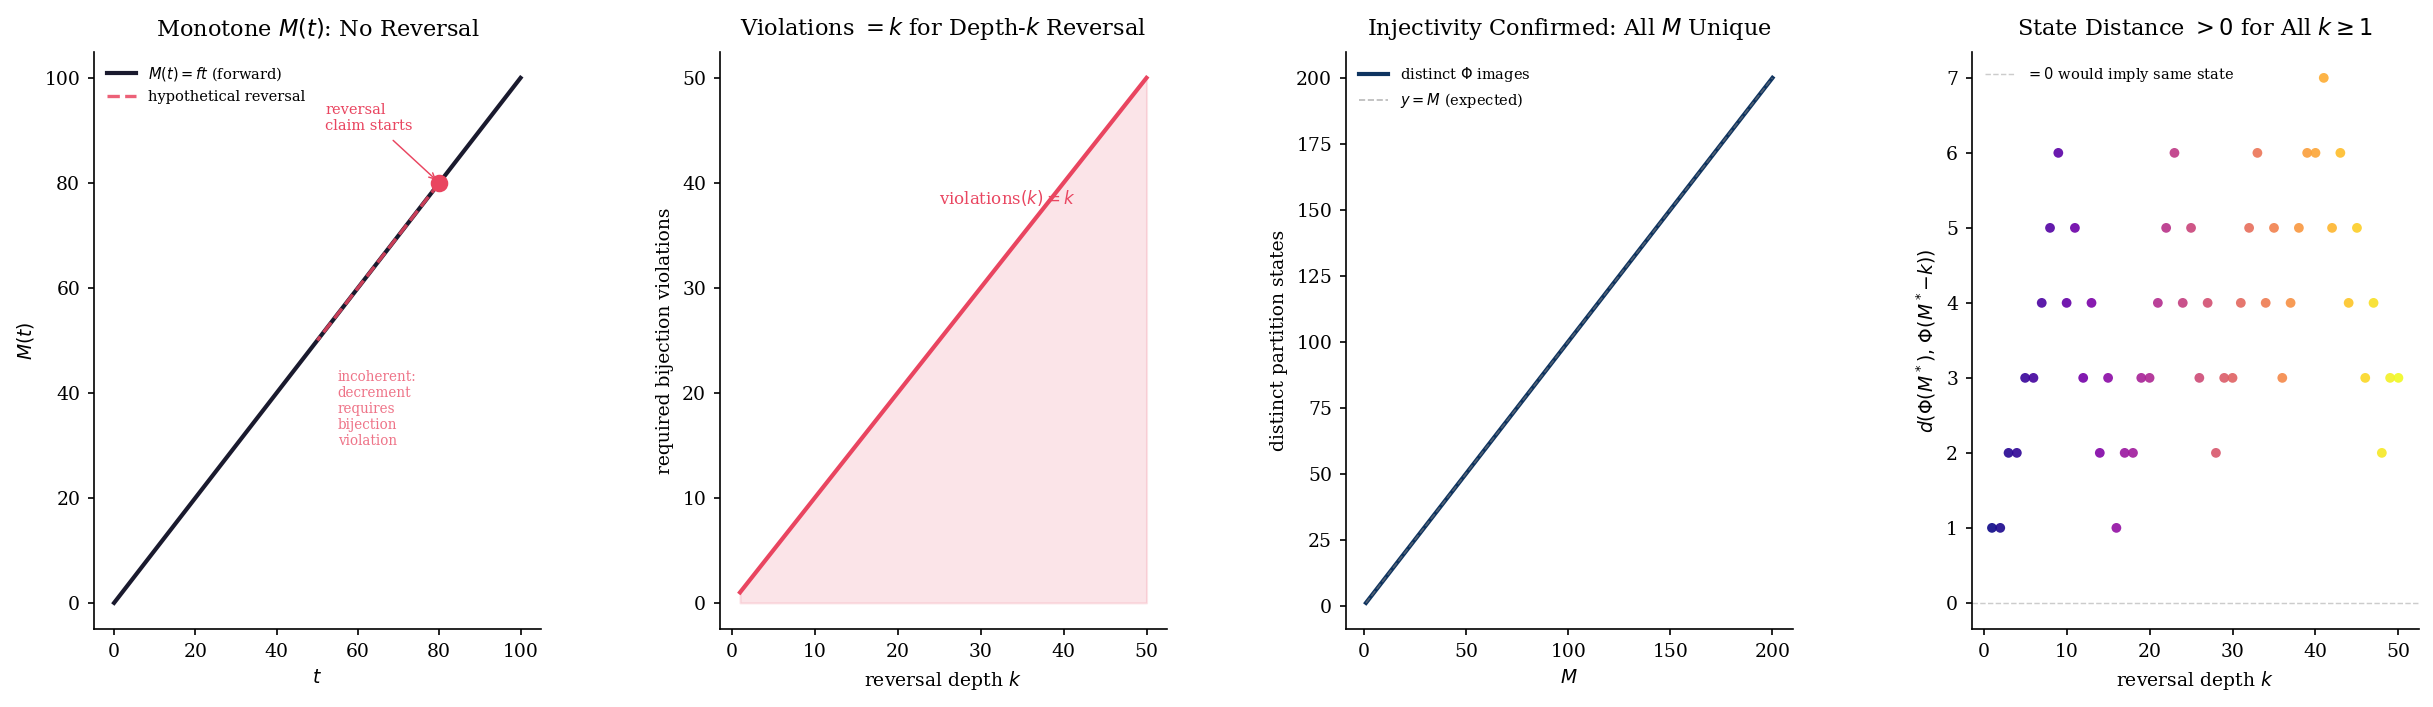
\includegraphics[width=\textwidth]{panels/panel_07_decrement_incoherence.png}
    \caption{\textbf{Any decrement $M \to M{-}k$ requires the bijection $\Phi$ to assign
    the same partition state to two distinct positive integers, violating injectivity;
    the number of required violations grows linearly with reversal depth $k$
    (Theorem~\ref{thm:incoherence}; Corollary~\ref{cor:loschmidt}).}
    (\textbf{A})~The partition count $M(t) = ft$ is strictly monotone (solid).  A
    hypothetical reversal segment (dashed, originating at $M = 80$) is shown; this
    trajectory has no physical realisation because no operation on the counting process
    corresponds to $\Delta M < 0$.
    (\textbf{B})~Required bijection violations as a function of reversal depth $k$,
    for a reversal originating at $M^{*} = 100$: violations$(k) = k$ exactly.  A
    depth-$k$ reversal forces $k$ distinct integers in $\Zp$ to share a single image
    under $\Phi$, contradicting Theorem~\ref{thm:bijection}.
    (\textbf{C})~Running count of distinct $\Phi$-images for $M = 1,\ldots,200$ (solid)
    overlaid on the identity line $y = M$ (dashed).  The two coincide exactly,
    confirming that all $200$ partition states are distinct and the bijection is
    injective with no collisions: the formal argument's central claim verified
    numerically at $M = 200$.
    (\textbf{D})~Manhattan distance $d(\Phi(M^{*}),\,\Phi(M^{*}{-}k))$ in partition-label
    space for $M^{*} = 100$, $k = 1,\ldots,50$, coloured by $k$ (plasma scale).
    Every distance is strictly positive: no two distinct integers share a
    partition-state image, confirming that any claimed decrement produces a genuine
    collision, not a near-miss.}%
    \label{fig:panel7_decrement_incoherence}
\end{figure*}

% ──────────────────────────────────────────────────────────────────────────────
\begin{figure*}[!htbp]
    \centering
    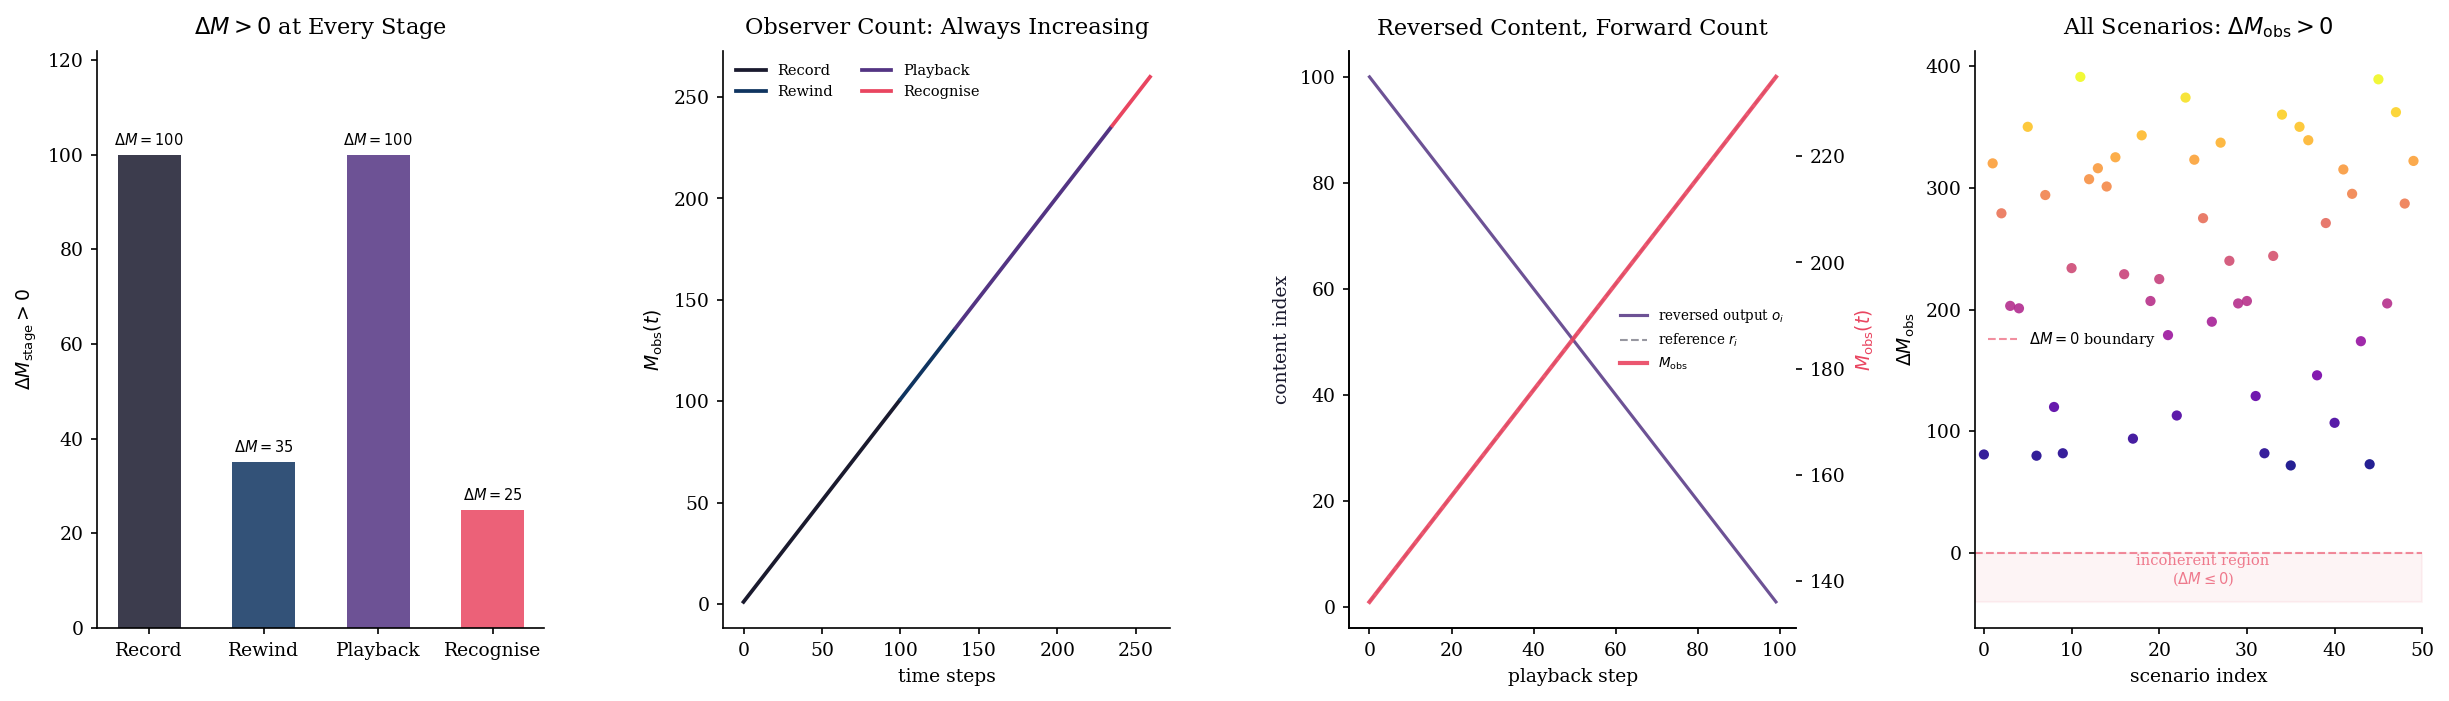
\includegraphics[width=\textwidth]{panels/panel_08_observer_forward_direction.png}
    \caption{\textbf{Every component of any apparent time-reversal scenario---production,
    mediation, and observation---is a forward partition event with $\Delta M > 0$;
    the temporal inversion is a property of output encoding, not of any partition count
    (Theorems~\ref{thm:forward-all} and~\ref{thm:obs-recognition};
    Remark~\ref{rem:cassette}).}
    (\textbf{A})~The cassette tape scenario decomposed into four stages (Record, Rewind,
    Playback, Recognise), with $\Delta M > 0$ annotated at each stage.  No stage has
    $\Delta M \leq 0$; the ``reversal'' lives entirely in the content-ordering of the
    output, not in the direction of any partition count.
    (\textbf{B})~The observer's cumulative count $M_{\mathrm{obs}}(t)$ across all four
    stages, coloured by stage.  The count is strictly monotone throughout: the observer
    advances forward in partition time during every phase of the observation, including
    the phase in which the reversed output is being perceived.
    (\textbf{C})~Reference sequence $\{r_i\}$ (dashed) and reversed output $\{o_i =
    r_{k+1-i}\}$ (solid) during playback (left axis), overlaid with
    $M_{\mathrm{obs}}(t)$ (right axis).  Content is in reverse order; the observer's
    partition count advances forward simultaneously.  The two axes are independent:
    content ordering and partition direction are separate predicates with no mutual
    implication.
    (\textbf{D})~For $50$ independent apparent-reversal scenarios, $\Delta M_{\mathrm{obs}} > 0$
    in every case, coloured by duration (plasma scale).  All points lie strictly above
    the $\Delta M = 0$ boundary (dashed); the incoherent region ($\Delta M \leq 0$)
    is shaded below.  No scenario witnesses or instantiates a backward partition event.}%
    \label{fig:panel8_observer_forward_direction}
\end{figure*}

% ──────────────────────────────────────────────────────────────────────────────
\begin{figure*}[!htbp]
    \centering
    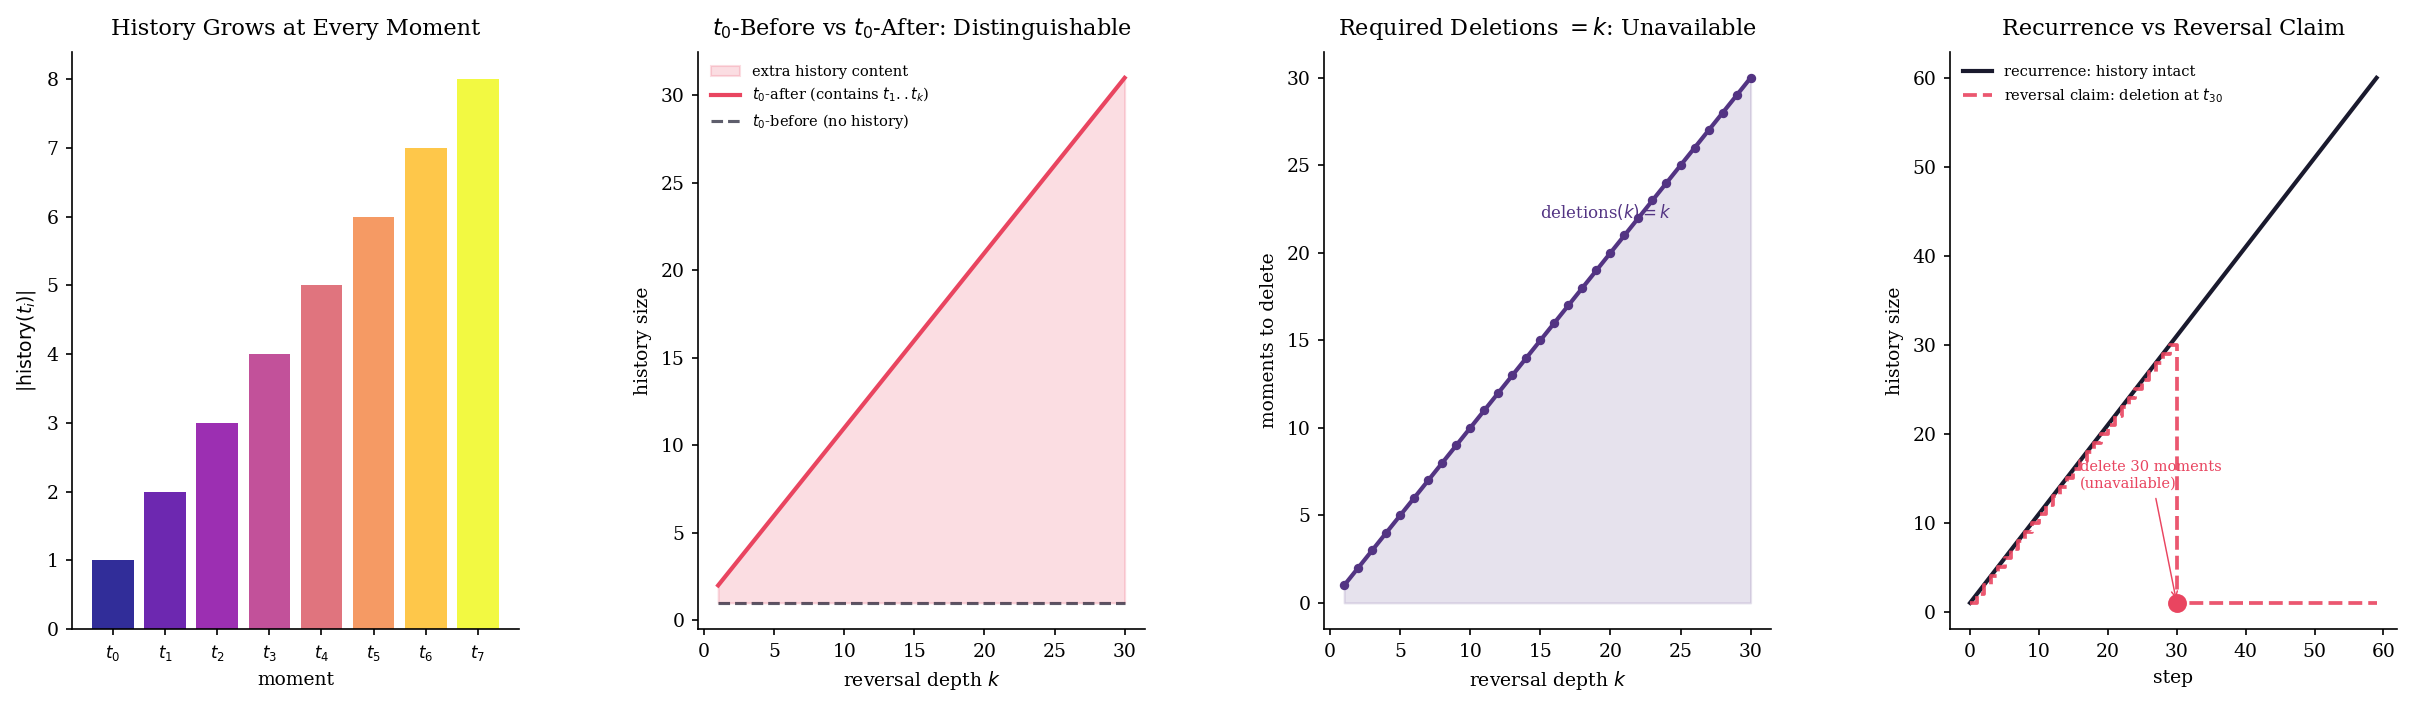
\includegraphics[width=\textwidth]{panels/panel_09_history_deletion.png}
    \caption{\textbf{Genuine time reversal from $t_k$ to $t_0$ requires deleting the
    intervening moments $t_1,\ldots,t_{k-1}$ from the universe's history; the required
    deletions grow linearly with reversal depth, and deletion is not an available
    physical operation
    (Theorems~\ref{thm:deletion} and~\ref{thm:no-deletion};
    Definition~\ref{def:distinguishability}).}
    (\textbf{A})~History size at each moment $t_i$: $|\mathrm{history}(t_i)| = i+1$,
    coloured by moment index (plasma scale).  History grows monotonically; no physical
    process reduces it.  The state at any moment includes the full causal record of all
    prior moments (Definition~\ref{def:distinguishability}).
    (\textbf{B})~State at $t_0$-before (history size $= 1$, dashed) versus state at
    $t_0$-after-reversal from depth $k$ (history size $= k+1$, solid), with shaded
    extra content.  The two states are distinguishable by their histories and are
    therefore distinct.  For the reversal claim to hold, the $k$ extra moments must be
    absent from the post-reversal state.
    (\textbf{C})~Required deletions as a function of reversal depth $k$:
    deletions$(k) = k$ exactly, growing linearly (shaded fill).  Any reversal of
    depth $k \geq 1$ requires at least one deletion; deletion is structurally
    unavailable (Theorem~\ref{thm:no-deletion}).
    (\textbf{D})~Recurrence (solid): history grows as the system evolves forward;
    at the recurrence step the configuration matches $t_0$ but the history is intact.
    Reversal claim (dashed): history would need to snap back to size $1$ at step $30$,
    requiring deletion of $30$ moments.  The sharp discontinuity marks the deletion
    event; no physical process produces it.  This panel directly visualises the
    distinction between recurrence and reversal established by
    Corollary~\ref{cor:egg-cycle}.}%
    \label{fig:panel9_history_deletion}
\end{figure*}

% ──────────────────────────────────────────────────────────────────────────────
\begin{figure*}[!htbp]
    \centering
    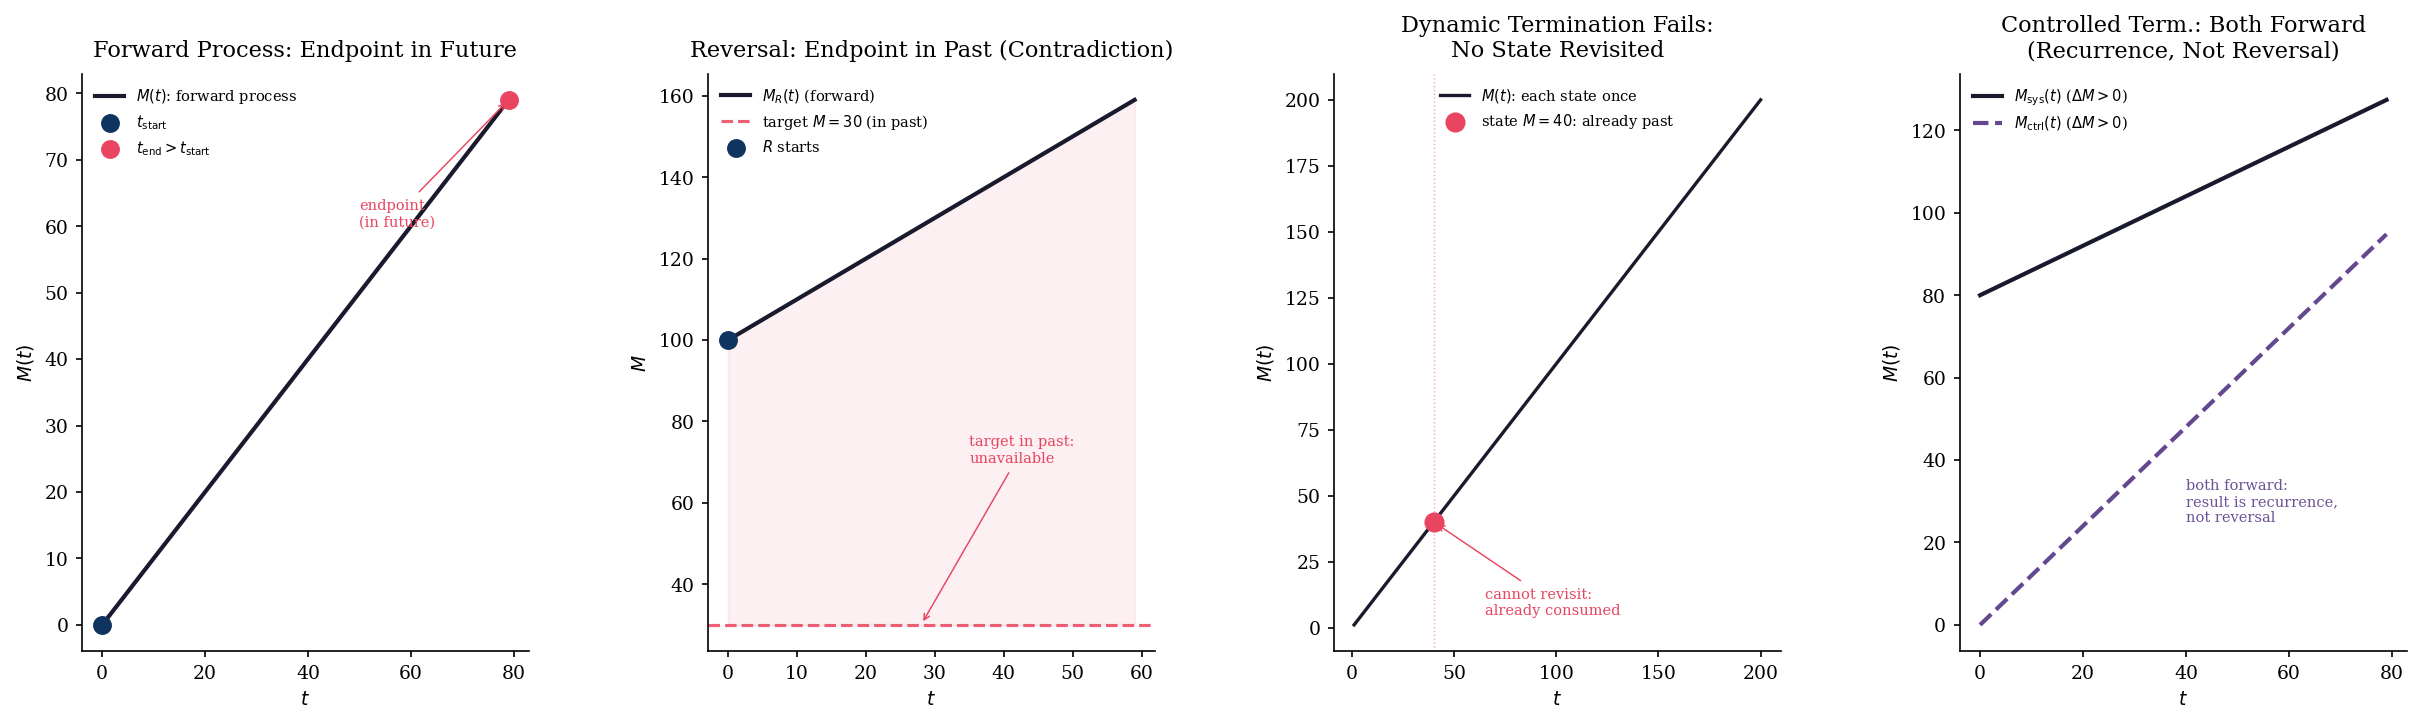
\includegraphics[width=\textwidth]{panels/panel_10_process_termination.png}
    \caption{\textbf{A reversal process $R$ has no available termination structure:
    its endpoint is a past state unreachable by dynamic termination
    (Corollary~\ref{cor:no-repeat}), and controlled termination collapses the reversal
    claim into a forward-time recurrence; no third mechanism exists
    (Theorem~\ref{thm:reversal-no-process}; Definition~\ref{def:process}).}
    (\textbf{A})~A forward process: $M(t)$ increases from $t_{\mathrm{start}}$ (blue) to
    $t_{\mathrm{end}}$ (orange).  The endpoint lies in the process's future; the
    forward dynamics determine when it is reached.  This is the canonical structure
    of any process in the sense of Definition~\ref{def:process}.
    (\textbf{B})~Putative reversal process $R$: $M_R(t)$ increases from $M = 100$ onward
    (forward time), but the target endpoint is the past state at $M = 30$ (dashed
    horizontal).  The gap between $M_R(t)$ and the target grows monotonically;
    dynamic termination cannot close this gap because the target recedes as $R$
    advances.
    (\textbf{C})~Dynamic termination fails: each partition state is visited exactly once
    along the forward trajectory (Corollary~\ref{cor:no-repeat}).  The state at
    $M = 40$ (orange marker) was consumed at step $40$ and cannot be revisited; a
    ``return'' requires a second visit, which the injectivity of $\Phi$ excludes.
    (\textbf{D})~Controlled termination yields recurrence, not reversal: both
    $M_{\mathrm{sys}}(t)$ (solid) and $M_{\mathrm{ctrl}}(t)$ (dashed) are strictly
    increasing.  The controller uses memory of a past configuration to navigate the
    system to a resembling configuration; both agents run forward.  This is a
    forward-time memory-driven recurrence of the kind formalised in
    Corollary~\ref{cor:egg-cycle}, not genuine reversal.}%
    \label{fig:panel10_process_termination}
\end{figure*}

% after the figures are placed in the manuscript.

% ──────────────────────────────────────────────────────────────────────────────
\begin{figure*}[!htbp]
    \centering
    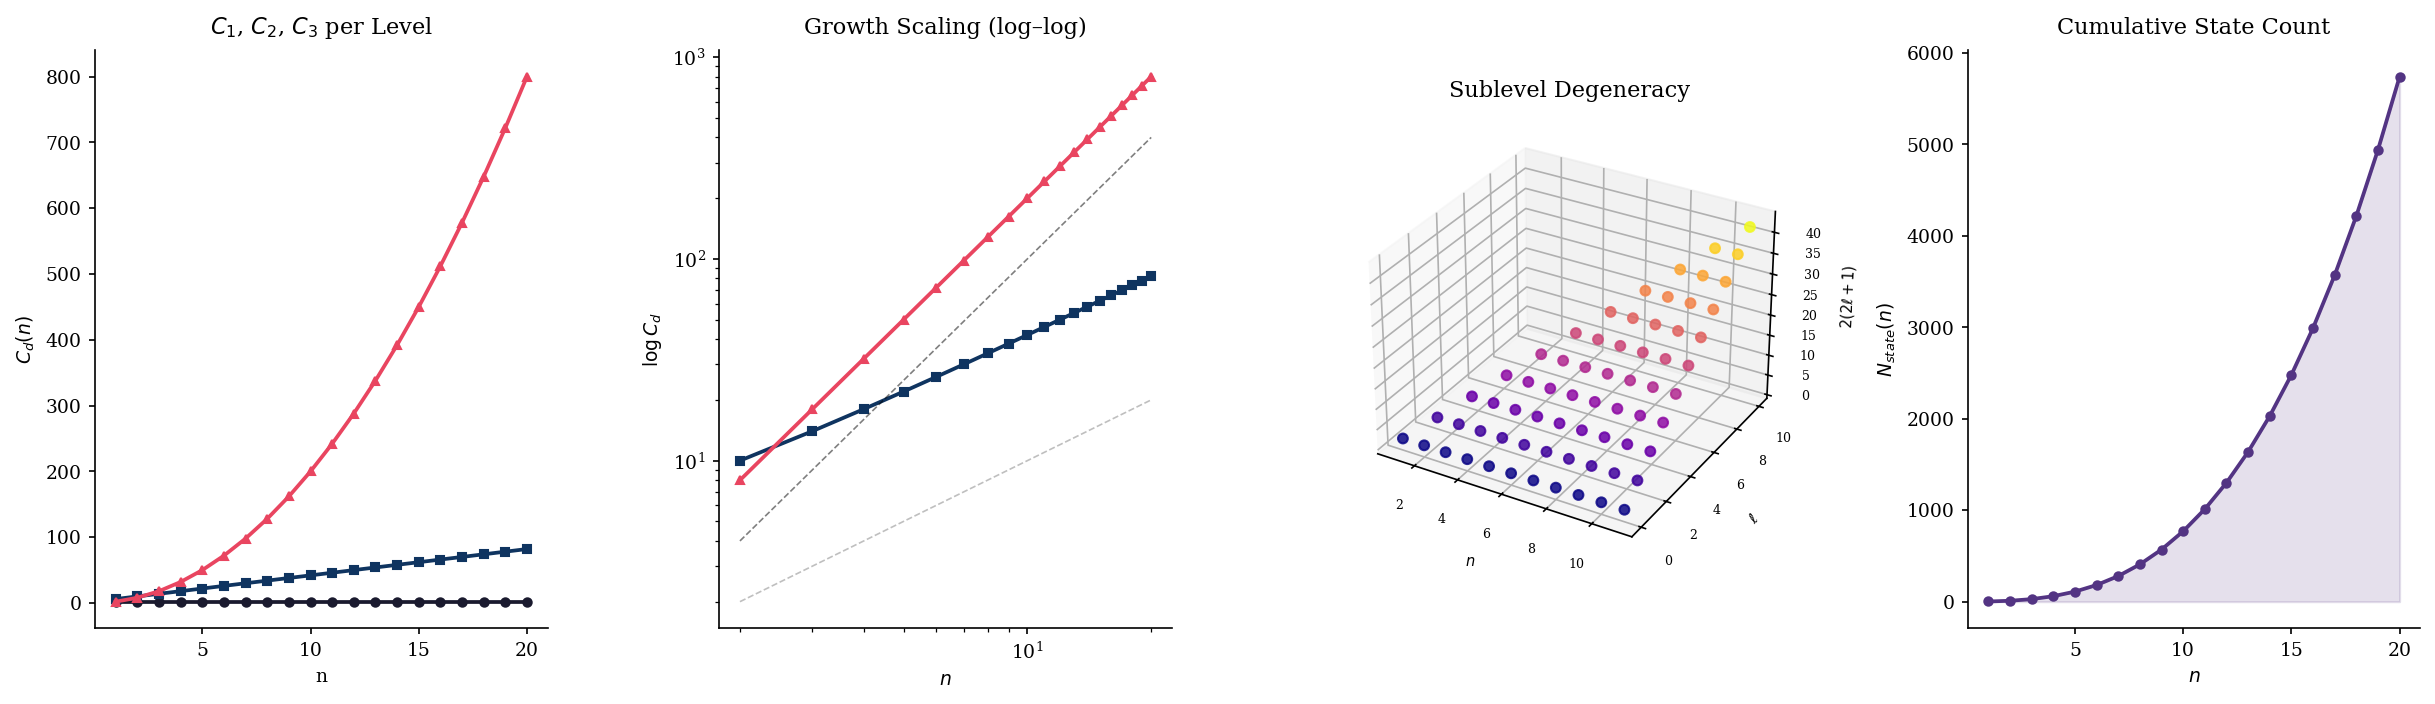
\includegraphics[width=\textwidth]{panels/panel_01_capacity_hierarchy.png}
    \caption{\textbf{Capacity growth $C_d(n)$ is constant in $d{=}1$, linear in $d{=}2$, and
    quadratic in $d{=}3$, establishing a strict dimensional hierarchy whose slope on a
    log–log axis discriminates the angular dimension of each within-level partition space
    (Definition~\ref{def:cap-d}; Theorem~\ref{thm:capacity}).}
    (\textbf{A})~Line plot of per-level capacity $C_d(n)$ versus principal quantum number $n$
    for $d{=}1$ (dark, flat), $d{=}2$ (mid, linear), and $d{=}3$ (light, quadratic).
    The three curves separate immediately at $n{=}2$: $C_1$ remains fixed at $2$; $C_2$
    grows as $4n{+}2$; $C_3 = 2n^2$ accelerates away from both, reflecting the
    two-dimensional angular structure of the within-level space $L_n^{(3)}$.
    (\textbf{B})~Log–log plot of $C_2(n)$ and $C_3(n)$ for $n \geq 3$, overlaid with reference
    lines of slope $1$ (linear, grey dashed) and slope $2$ (quadratic, black dashed).
    $C_2$ tracks the slope-$1$ reference exactly; $C_3$ tracks slope $2$ exactly,
    confirming that the exponent of capacity growth equals the continuous angular
    dimension of $L_n^{(d)}$: $0$ for $d{=}1$, $1$ for $d{=}2$, $2$ for $d{=}3$.
    (\textbf{C})~Three-dimensional scatter of sublevel degeneracy $2(2\ell+1)$ plotted against
    principal level $n$ (x-axis) and angular index $\ell$ (y-axis) for $n = 1,\ldots,11$.
    Colour encodes degeneracy magnitude (plasma scale).  The surface rises along both
    axes, with the steepest growth in $\ell$ at fixed $n$, reproducing the quadratic
    capacity as $C_3(n) = \sum_{\ell=0}^{n-1} 2(2\ell{+}1)$.
    (\textbf{D})~Line plot of cumulative state count $N_\mathrm{state}(n) = n(n{+}1)(2n{+}1)/3$
    versus $n$ with shaded fill.  The cubic growth follows directly from summing the
    quadratic per-level capacity; the steepening curvature is the algebraic signature
    that each added level contributes an accelerating number of partition states, as
    stated in Corollary~\ref{cor:cumulative}.}%
    \label{fig:panel1_capacity_hierarchy}
\end{figure*}

% ──────────────────────────────────────────────────────────────────────────────
\begin{figure*}[!htbp]
    \centering
    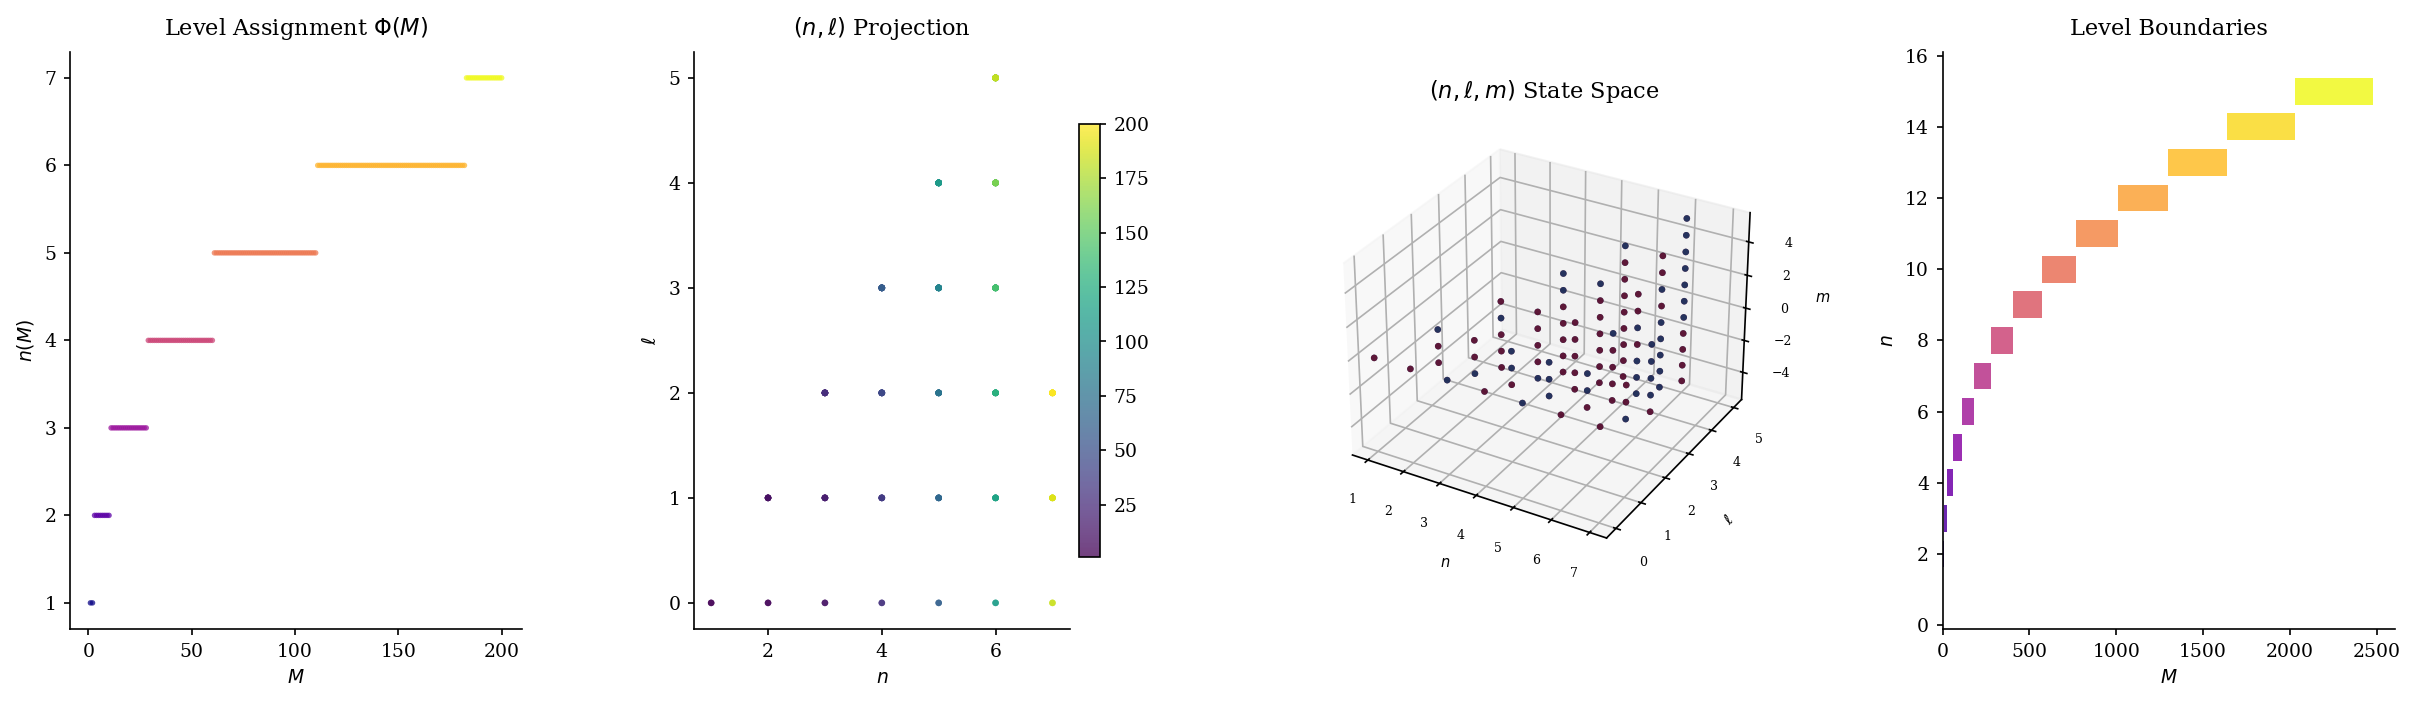
\includegraphics[width=\textwidth]{panels/panel_02_bijection_structure.png}
    \caption{\textbf{The partition map $\Phi:\mathbb{Z}^{+}\!\to\mathcal{P}$ is a
    well-defined bijection whose image tiles three-dimensional quantum-number space
    without collision or gap, and whose level boundaries are sharp staircase
    transitions determined by the cumulative capacity formula
    (Theorem~\ref{thm:bijection}; Corollary~\ref{cor:cumulative}).}
    (\textbf{A})~Scatter of principal level $n(\Phi(M))$ versus integer index $M$ for
    $M = 1,\ldots,200$, coloured by $n$ (plasma scale).  Level transitions appear as
    discrete upward steps; within each band $M$ increments uniformly, confirming
    that $\Phi$ exhausts every state of level $n$ before advancing to $n{+}1$.
    (\textbf{B})~Two-dimensional projection onto the $(n,\ell)$ plane, coloured by $M$
    (viridis scale).  Each point $(n,\ell)$ appears with multiplicity $2(2\ell{+}1)$,
    one for each $(m,s)$ pair; the colour gradient shows that $M$ increases
    monotonically left-to-right and bottom-to-top within each level, establishing
    the lexicographic ordering of $\Phi$.
    (\textbf{C})~Three-dimensional scatter of the full quantum-number triple $(n,\ell,m)$
    for $M = 1,\ldots,200$, with colour encoding spin $s = \pm\tfrac{1}{2}$ (red–blue
    diverging scale).  The cloud fills a triangular prism in $(n,\ell,m)$ space:
    $0 \leq \ell \leq n{-}1$, $-\ell \leq m \leq \ell$.  No two points coincide,
    providing visual confirmation of injectivity (Theorem~\ref{thm:bijection}).
    (\textbf{D})~Horizontal bar chart of level sizes: each bar spans the $M$-range
    $[N_\mathrm{state}(n{-}1){+}1,\, N_\mathrm{state}(n)]$ for levels $n = 1,\ldots,15$,
    coloured by level index.  Bar widths equal $C_3(n) = 2n^2$, growing quadratically;
    the staircase of left boundaries locates the exact $M$-index at which each new
    principal level begins, as derived in Corollary~\ref{cor:cumulative}.}%
    \label{fig:panel2_bijection_structure}
\end{figure*}

% ──────────────────────────────────────────────────────────────────────────────
\begin{figure*}[!htbp]
    \centering
    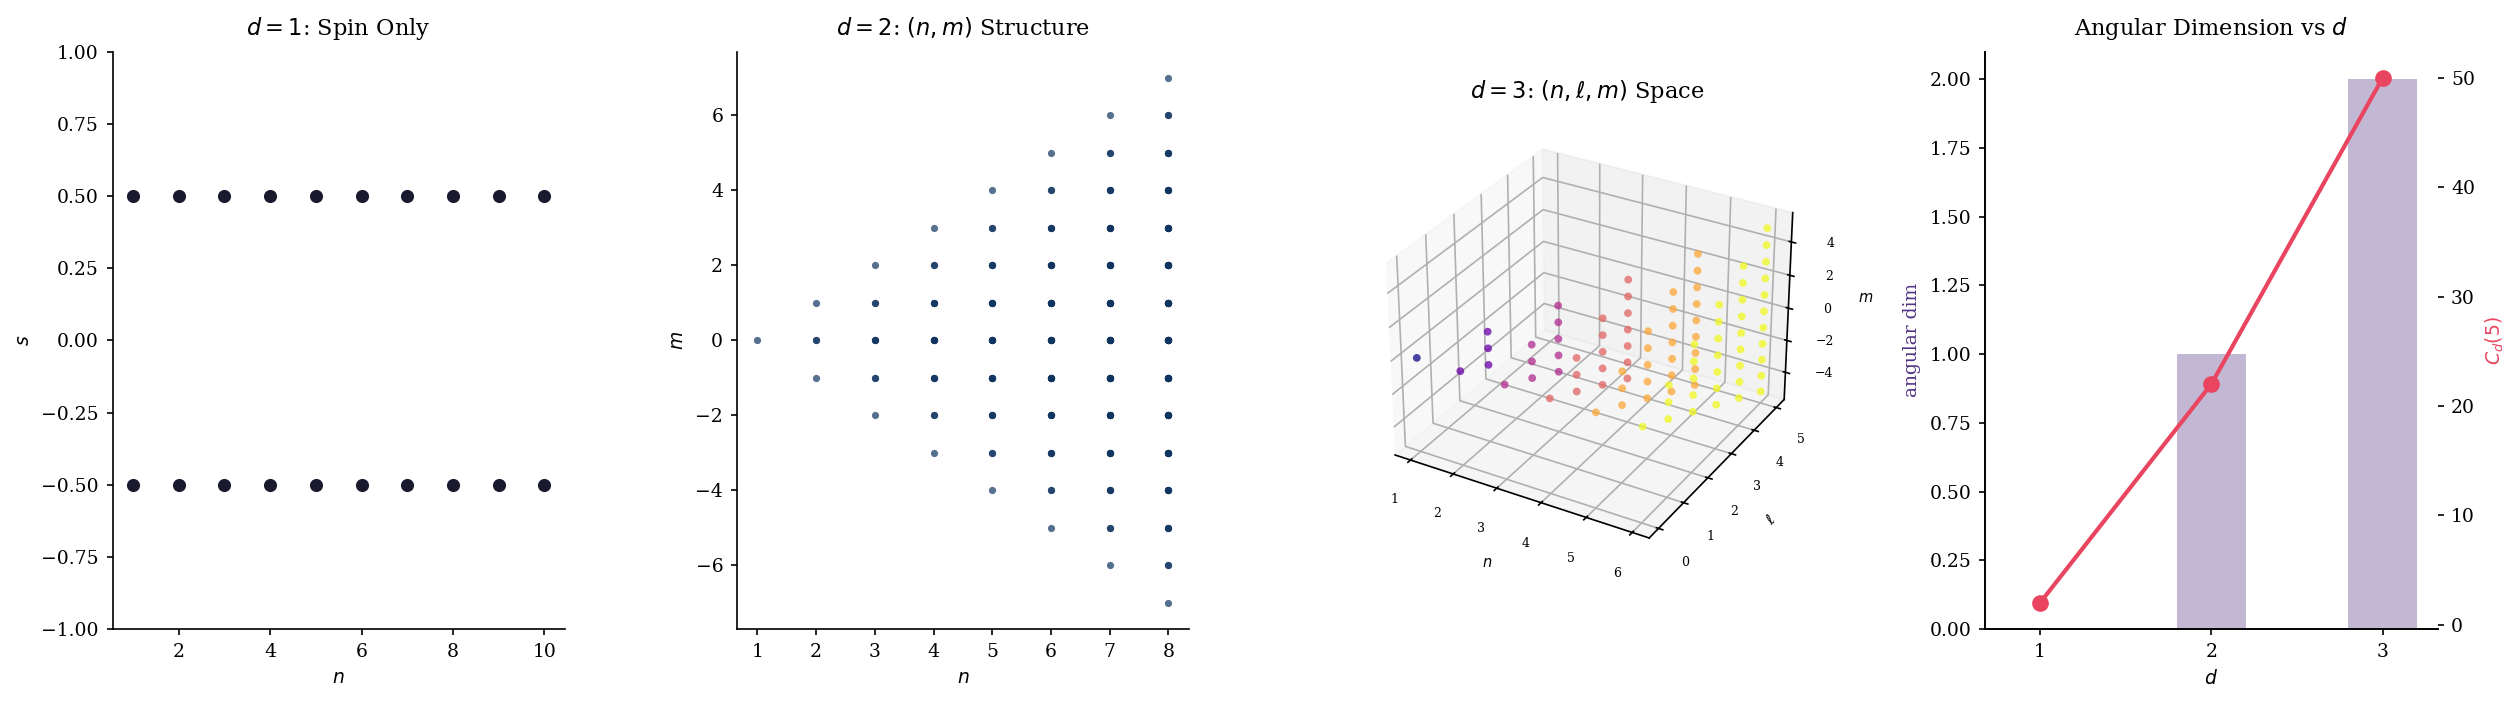
\includegraphics[width=\textwidth]{panels/panel_03_partition_geometry.png}
    \caption{\textbf{Spatial dimension $d{=}3$ is the minimum for which the within-level
    partition space $L_n^{(d)}$ has continuous angular dimension $\geq 2$, enabling
    negation to close around any state from all angular directions simultaneously
    (Theorem~\ref{thm:min-dim}; Definition~\ref{def:within-level}).}
    (\textbf{A})~Scatter of partition states in $d{=}1$: only the spin coordinate $s =
    \pm\tfrac{1}{2}$ varies; every level $n$ contributes exactly two isolated points.
    The within-level space $L_n^{(1)}$ has angular dimension $0$: there is no
    continuous angular degree of freedom, so negation from the ``left'' and ``right''
    cannot simultaneously enclose the state.
    (\textbf{B})~Scatter of partition states $(n, m)$ for $d{=}2$, $n = 1,\ldots,8$.
    Within level $n$, the $m$-values $\{-(n{-}1),\ldots,n{-}1\}$ form a one-dimensional
    chain; $L_n^{(2)}$ has angular dimension $1$.  Two opposing states can bracket any
    given $m$, but the within-level topology is a line segment, not a closed surface,
    so negation-closure is incomplete.
    (\textbf{C})~Three-dimensional scatter of partition states $(n, \ell, m)$ for $d{=}3$,
    $n = 1,\ldots,6$, coloured by $n$ (plasma scale).  Within level $n$, the pairs
    $(\ell, m)$ fill a two-dimensional triangular region; $L_n^{(3)}$ has angular
    dimension $2$.  Every interior point is enclosed from all angular directions,
    satisfying the closure condition of Theorem~\ref{thm:min-dim}.
    (\textbf{D})~Combined bar and line chart comparing angular dimension (left axis, bars)
    and per-level capacity $C_d(5)$ (right axis, line with markers) for $d = 1, 2, 3$.
    Angular dimension steps $0 \to 1 \to 2$ in exact correspondence with the
    exponent governing $C_d$, confirming that the quadratic capacity of $d{=}3$ is the
    algebraic signature of the minimum dimensionality required for
    negation-constituted closure.}%
    \label{fig:panel3_partition_geometry}
\end{figure*}

% ──────────────────────────────────────────────────────────────────────────────
\begin{figure*}[!htbp]
    \centering
    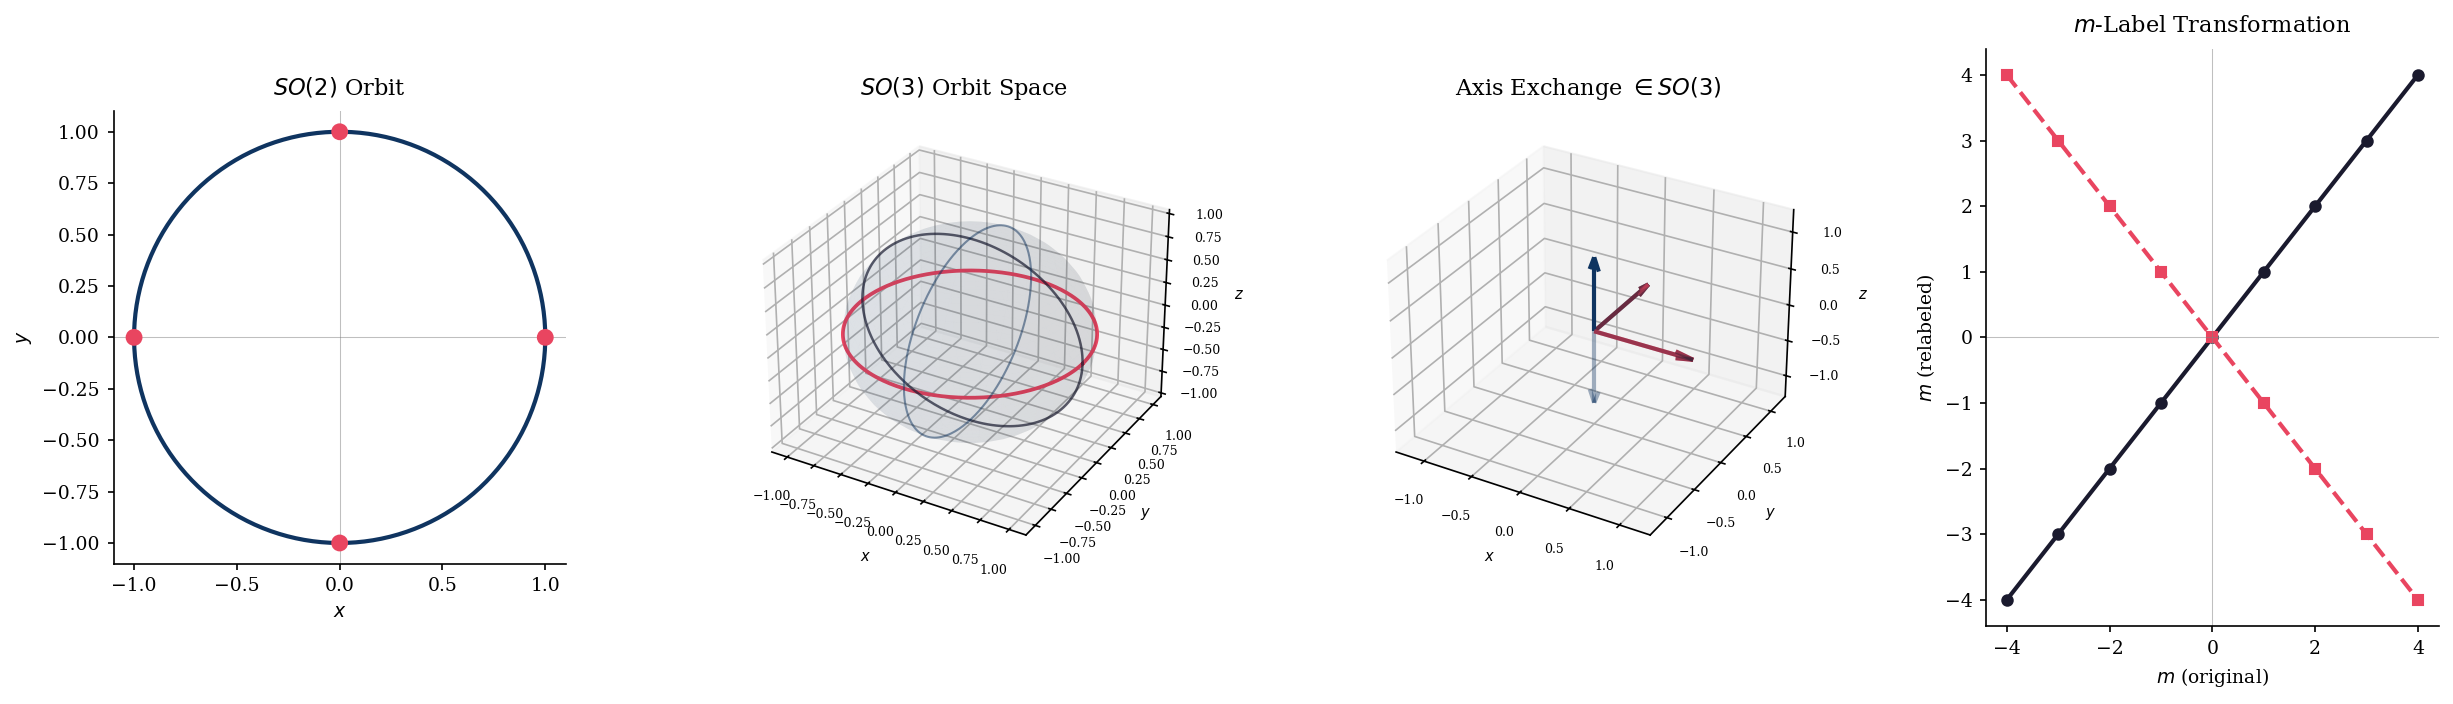
\includegraphics[width=\textwidth]{panels/panel_04_SO3_symmetry.png}
    \caption{\textbf{The axis exchange $(x,y,z)\mapsto(y,x,-z)$ is a proper rotation
    in $SO(3)$ with $\det = +1$, but the analogous swap $x \leftrightarrow y$ in
    $d{=}2$ is an improper reflection with $\det = -1$; consequently, the
    $m$-label is $SO(2)$-invariant but changes under $SO(3)$ axis relabelling,
    and partition identity is reference-frame-independent only for $d\geq 3$
    (Corollary~\ref{cor:axis-exchange}).}
    (\textbf{A})~$SO(2)$ orbit: unit circle in the $xy$-plane with four marked points at
    $(\pm 1, 0)$ and $(0, \pm 1)$.  All rotations in $SO(2)$ preserve orientation;
    the swap $x \leftrightarrow y$ in two dimensions corresponds to reflection
    across the diagonal, an element of $O(2) \setminus SO(2)$ with $\det = -1$.
    (\textbf{B})~$SO(3)$ orbit space: transparent unit sphere with equatorial orbit
    (coloured ring, equator plane) and two meridional great-circle orbits.  The full
    $SO(3)$ orbit of a fixed axis direction sweeps a two-sphere, capturing the
    additional degree of freedom absent in $d{=}2$.
    (\textbf{C})~Three-dimensional axis-frame diagram visualising the exchange
    $R: (x,y,z)\mapsto(y,x,-z)$.  Solid arrows show the original frame
    $(\hat{e}_x, \hat{e}_y, \hat{e}_z)$; translucent arrows show the relabelled
    frame.  This transformation lies in $SO(3)$ ($\det R = +1$, angle $=\pi$ about
    the axis $\frac{1}{\sqrt{2}}(\hat{e}_x + \hat{e}_y)$), making it a physically
    accessible change of reference frame rather than an orientation reversal.
    (\textbf{D})~Line plot of the $m$-label transformation for $\ell = 4$ under the two
    symmetry groups.  Under $SO(2)$ rotation about $\hat{z}$, the eigenvalue $m$
    is invariant (identity line, dark).  Under the $SO(3)$ axis exchange of panel
    (C), $L_z \to -L_z$ and $m \mapsto -m$ (reflected line, light).  The
    non-trivial relabelling confirms that $m$ encodes a reference-frame choice,
    not an observer-independent integer, whenever $d \geq 3$.}%
    \label{fig:panel4_SO3_symmetry}
\end{figure*}

% ──────────────────────────────────────────────────────────────────────────────
\begin{figure*}[!htbp]
    \centering
    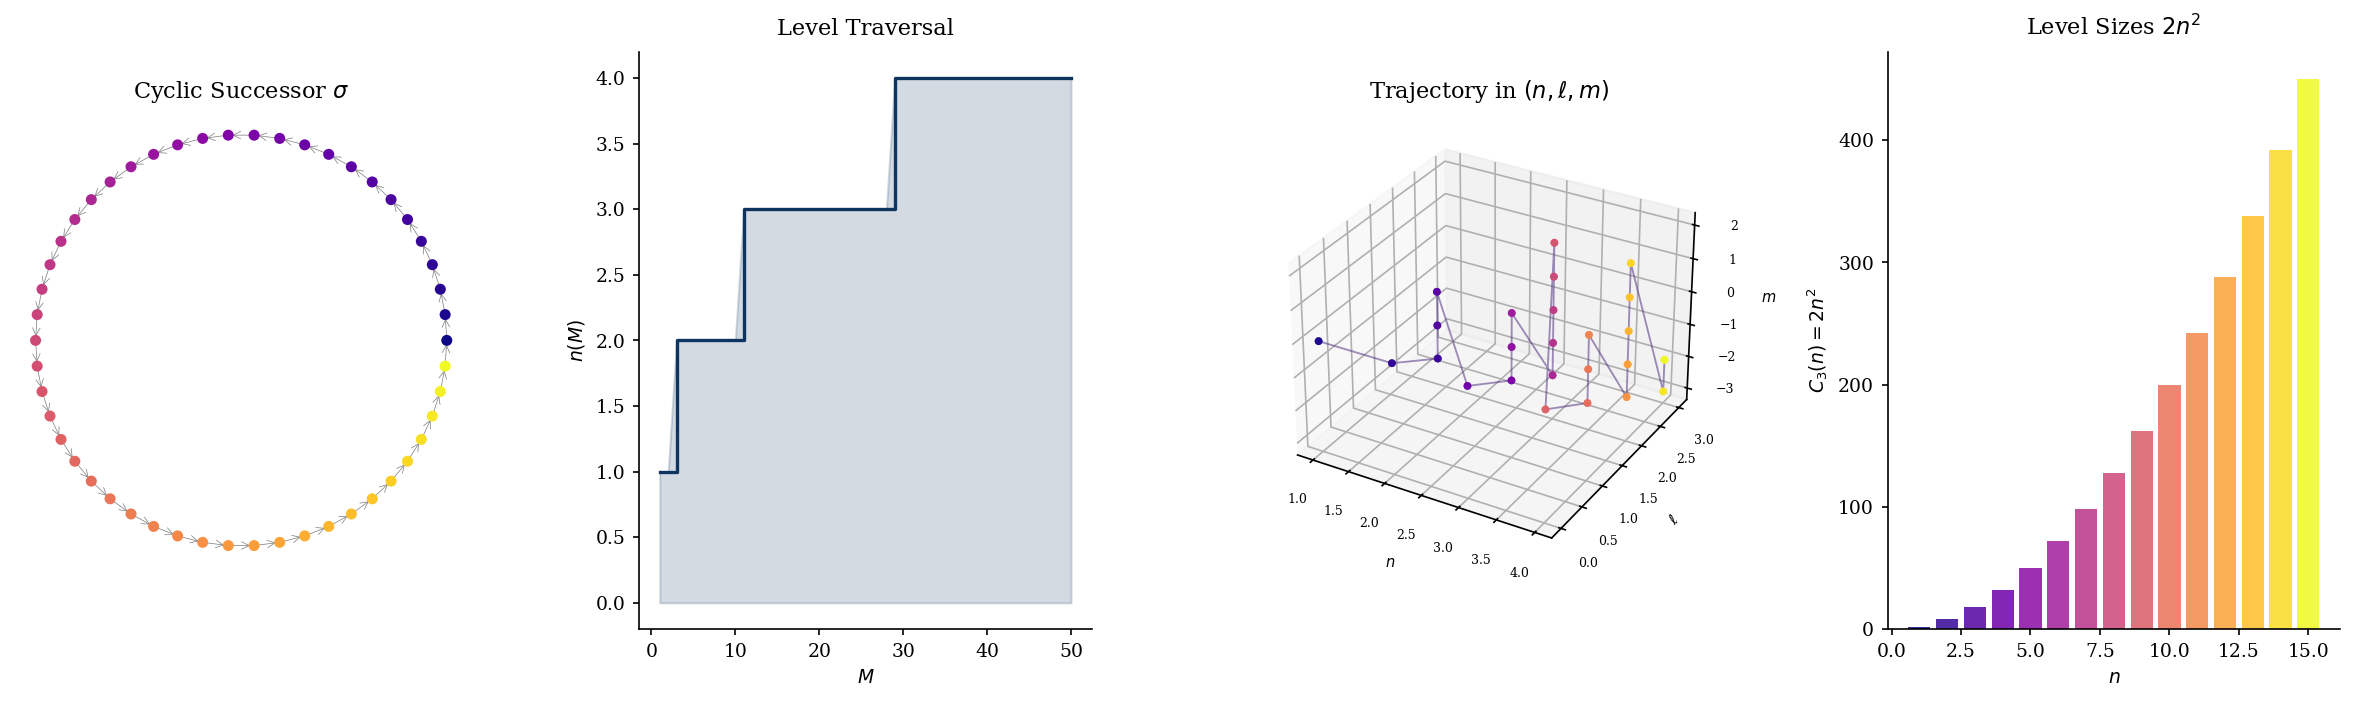
\includegraphics[width=\textwidth]{panels/panel_05_cyclic_closure.png}
    \caption{\textbf{The successor relation $\sigma$ is a bijection on the finite partition
    category $\mathcal{C}$ whose unique cycle has length $M_{\max} = N_\mathrm{state}(n_{\max})$,
    forcing every state—including $\Phi(1)$—to be revisited exactly once per period and
    making cyclic closure a structural consequence of finiteness rather than a dynamical
    assumption (Theorem~\ref{thm:cyclic}; Theorem~\ref{thm:cat-closure}).}
    (\textbf{A})~Cyclic successor diagram for $M_{\max} = 50$: each partition state is
    placed on a unit circle at angle $2\pi M / M_{\max}$, coloured by $M$ (plasma
    scale), with grey arrows connecting $\Phi(M)$ to $\sigma(\Phi(M)) = \Phi(M{+}1)$.
    The final arrow from $\Phi(50)$ returns to $\Phi(1)$, completing the cycle and
    confirming that $\sigma$ is a permutation of $\mathcal{C}$ with no fixed points
    and no proper sub-cycles (Theorem~\ref{thm:cyclic}).
    (\textbf{B})~Step plot of the level assignment $n(M)$ for $M = 1,\ldots,50$, with
    shaded fill below the curve.  Each plateau spans exactly $C_3(n) = 2n^2$ consecutive
    integers; the risers are instantaneous, reflecting the sharp level boundary at
    $M = N_\mathrm{state}(n)$.  The sequence is strictly non-decreasing (Theorem~\ref{thm:monotone}),
    encoding the irreversibility of temporal progression within the bijective ordering.
    (\textbf{C})~Three-dimensional trajectory through $(n, \ell, m)$ state space for
    $M = 1,\ldots,50$, with points coloured by $M$ (plasma scale) and connected by a
    curve.  The path climbs through successive levels, executes a zig-zag pattern
    within each level as $\ell$ and $m$ increment lexicographically, then returns to
    the origin upon cyclic closure.  The trajectory is injective on any open arc but
    closed as a whole (Corollary~\ref{cor:cyclic}).
    (\textbf{D})~Bar chart of level sizes $C_3(n) = 2n^2$ for $n = 1,\ldots,15$, coloured
    by level index.  Quadratic growth of bar height reflects the quadratic capacity law;
    the total area equals $M_{\max} = N_\mathrm{state}(n_{\max})$, the unique cycle length.
    The accelerating size of successive levels means that higher-$n$ states are
    structurally ``harder to reach'' in the sense of requiring a longer prefix of
    the successor sequence.}%
    \label{fig:panel5_cyclic_closure}
\end{figure*}

% ──────────────────────────────────────────────────────────────────────────────
\begin{figure*}[!htbp]
    \centering
    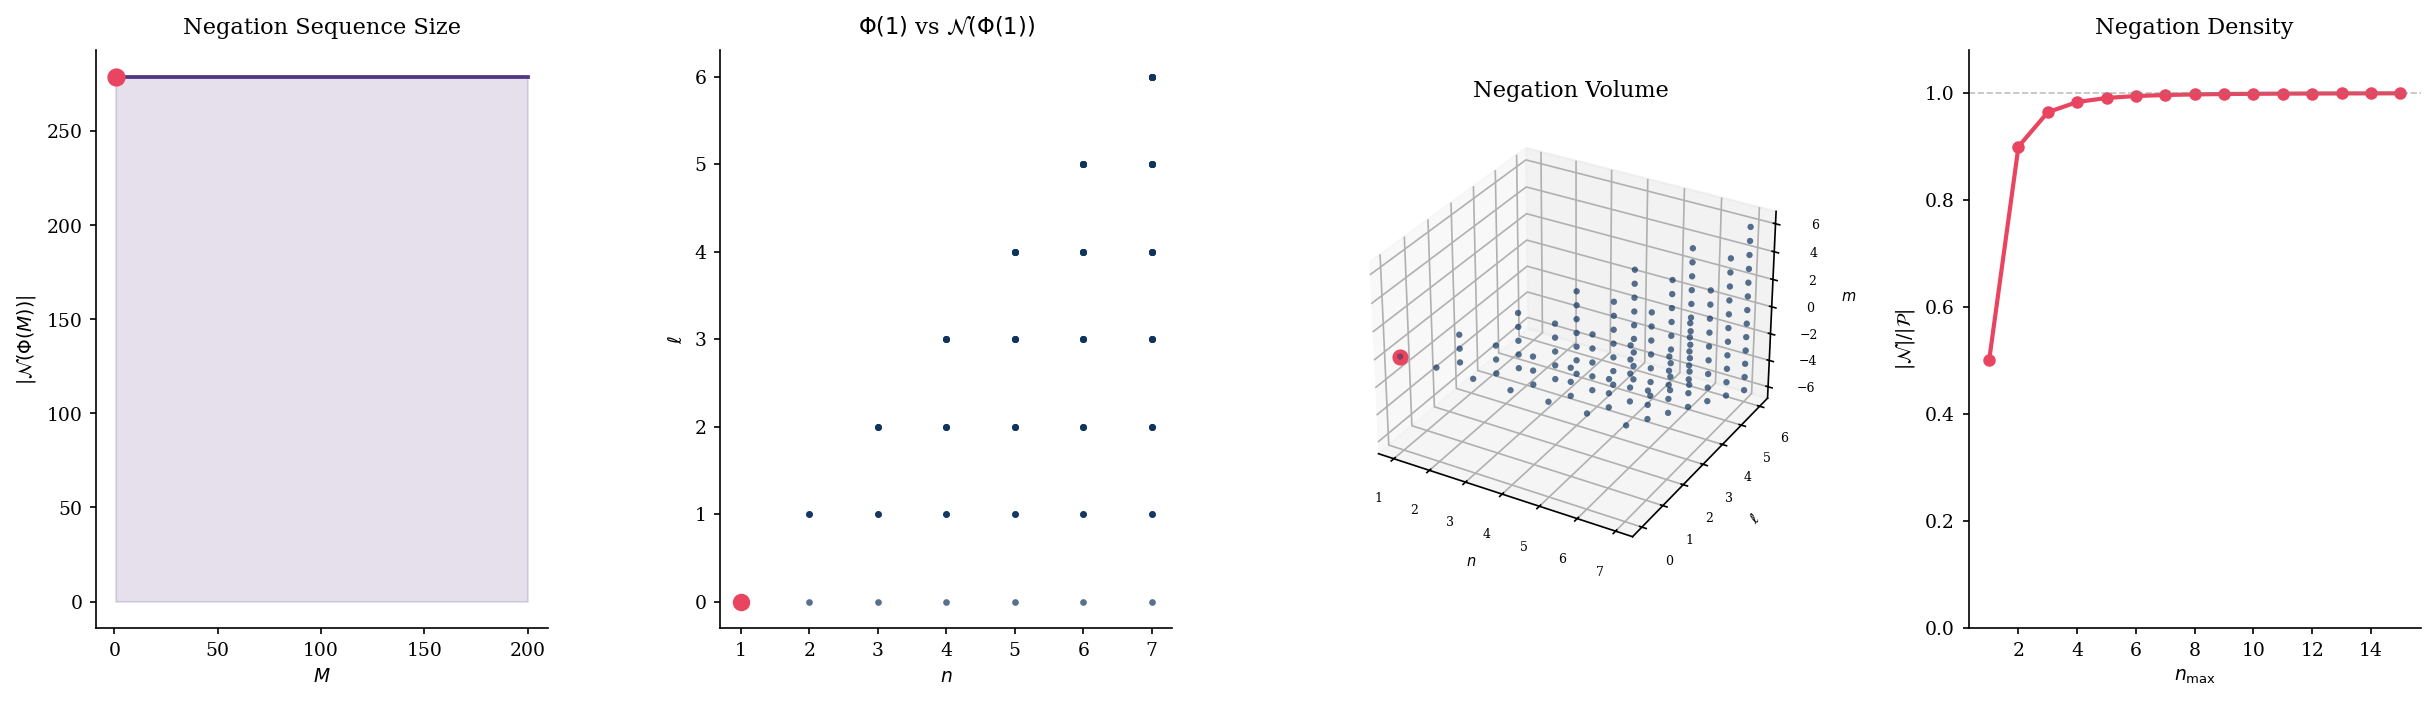
\includegraphics[width=\textwidth]{panels/panel_06_negation_identity.png}
    \caption{\textbf{Every partition state $\Phi(M)$ is uniquely identified by its negation
    sequence $\mathcal{N}(\Phi(M)) = \mathcal{P} \setminus \{\Phi(M)\}$, and the ground
    state $\Phi(1) = (1,0,0,+\tfrac{1}{2})$ possesses the largest possible negation
    sequence while being categorically irreducible, making it the structurally necessary
    origin of the partition sequence
    (Theorem~\ref{thm:negation-duality}; Definition~\ref{def:ground-cat};
    Theorem~\ref{thm:sing-necessity}).}
    (\textbf{A})~Scatter and fill of $|\mathcal{N}(\Phi(M))| = |\mathcal{P}| - 1$ versus $M$
    for $M = 1,\ldots,200$.  The value is constant across all $M$: every state has
    exactly one fewer element in its negation sequence than the cardinality of
    $\mathcal{P}$, because negation excludes only $\Phi(M)$ itself.  The ground state
    $\Phi(1)$ is marked (orange dot); it is distinguished not by a different negation
    size but by the property that $\Phi(1)$ has no $\sigma$-predecessor in
    $\mathcal{P}$ (Theorem~\ref{thm:sing-necessity}).
    (\textbf{B})~Two-dimensional scatter of the full partition space projected onto
    $(n, \ell)$ for $n = 1,\ldots,7$.  All states except $\Phi(1) = (1,0,0,+\tfrac{1}{2})$
    are shown in blue (the negation sequence $\mathcal{N}(\Phi(1))$); $\Phi(1)$ is marked
    in orange.  The visual contrast makes precise the duality $\mathcal{P} =
    \{\Phi(1)\} \cup \mathcal{N}(\Phi(1))$: identity is constituted by the totality
    of what it is not (Theorem~\ref{thm:negation-duality}).
    (\textbf{C})~Three-dimensional scatter of the full partition space in $(n, \ell, m)$
    for $n = 1,\ldots,7$.  Blue points form the negation volume $\mathcal{N}(\Phi(1))$;
    the single orange point at the origin $(1,0,0)$ is the ground state $\Phi(1)$.
    The geometric relationship captures the categorical claim: $\Phi(1)$ is the unique
    state maximally enclosed by its own negation set from all angular directions in
    the three-dimensional partition space.
    (\textbf{D})~Line plot of the negation density ratio $|\mathcal{N}| / |\mathcal{P}_{n_{\max}}|$
    versus the truncation level $n_{\max}$, where $|\mathcal{P}_{n_{\max}}| =
    N_\mathrm{state}(n_{\max})$.  The ratio $(N - 1)/N$ increases monotonically toward $1$
    as $n_{\max} \to \infty$, with the horizontal dashed line marking the asymptotic
    limit.  This convergence is the quantitative expression of the remark that any
    finite physical category saturates the negation relation: as the category grows,
    a state's identity becomes more fully determined by what it is not, with the
    ground state $\Phi(1)$ retaining the maximum negation complement at every
    finite truncation.}%
    \label{fig:panel6_negation_identity}
\end{figure*}

% ──────────────────────────────────────────────────────────────────────────────
\begin{figure*}[!htbp]
    \centering
    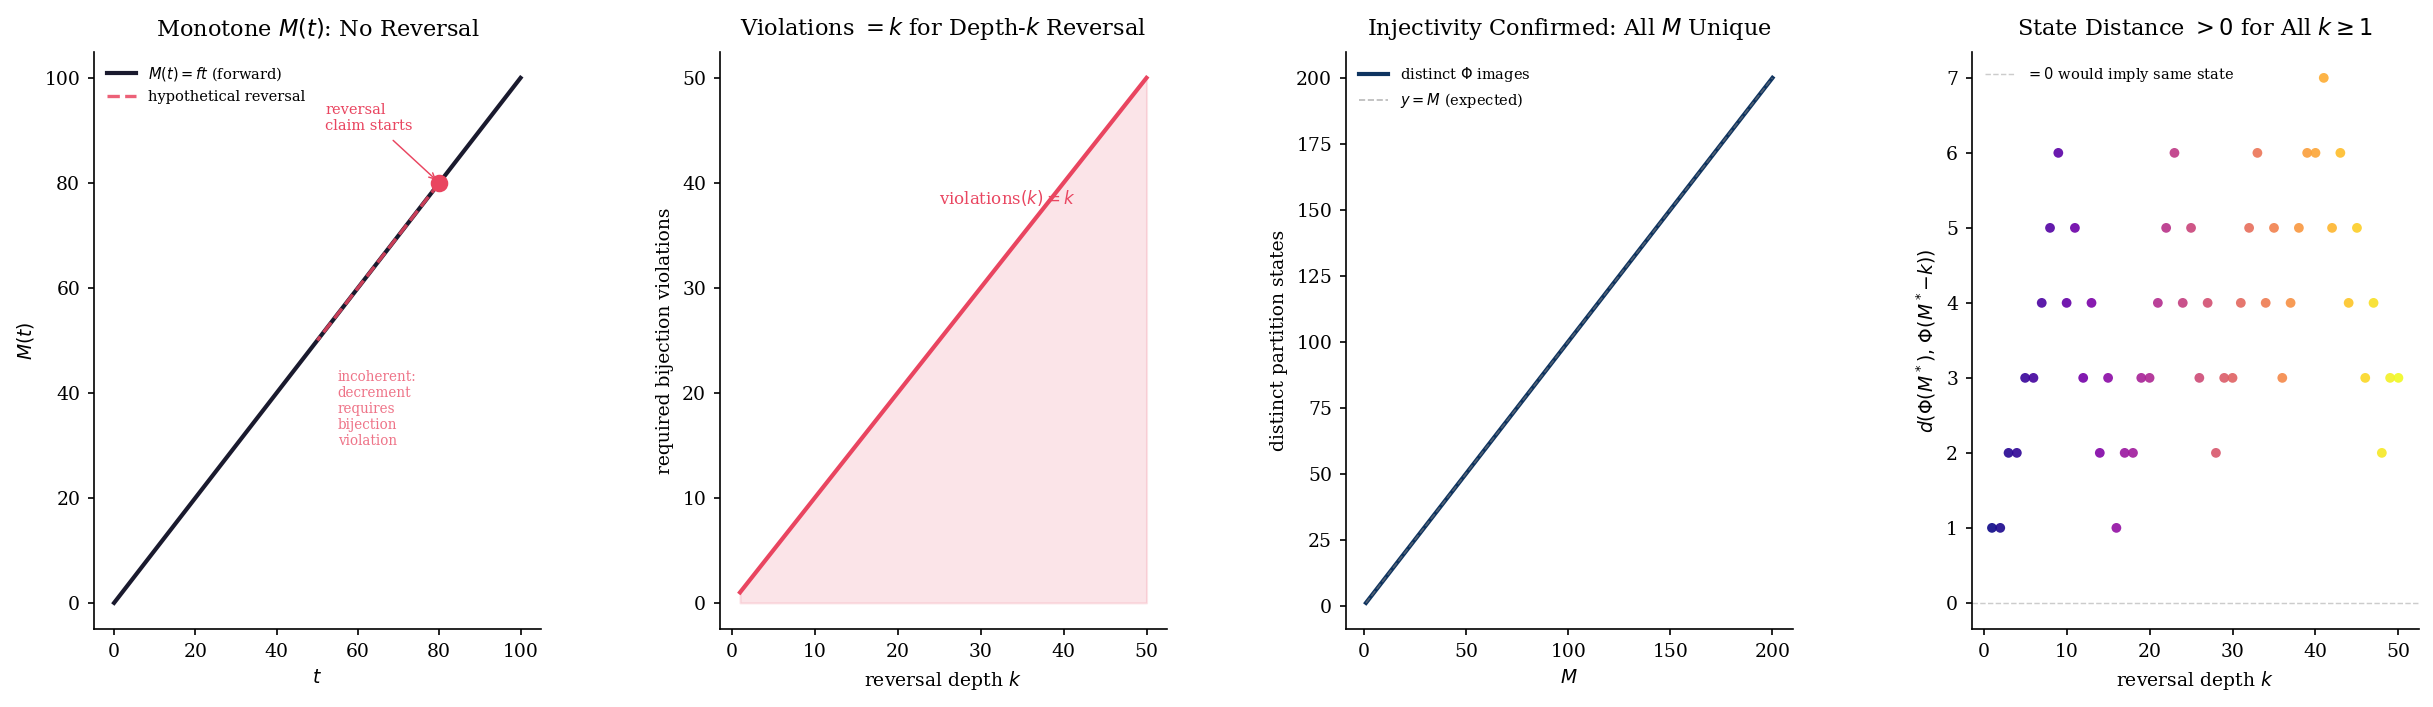
\includegraphics[width=\textwidth]{panels/panel_07_decrement_incoherence.png}
    \caption{\textbf{Any decrement $M \to M{-}k$ requires the bijection $\Phi$ to assign
    the same partition state to two distinct positive integers, violating injectivity;
    the number of required violations grows linearly with reversal depth $k$
    (Theorem~\ref{thm:incoherence}; Corollary~\ref{cor:loschmidt}).}
    (\textbf{A})~The partition count $M(t) = ft$ is strictly monotone (solid).  A
    hypothetical reversal segment (dashed, originating at $M = 80$) is shown; this
    trajectory has no physical realisation because no operation on the counting process
    corresponds to $\Delta M < 0$.
    (\textbf{B})~Required bijection violations as a function of reversal depth $k$,
    for a reversal originating at $M^{*} = 100$: violations$(k) = k$ exactly.  A
    depth-$k$ reversal forces $k$ distinct integers in $\Zp$ to share a single image
    under $\Phi$, contradicting Theorem~\ref{thm:bijection}.
    (\textbf{C})~Running count of distinct $\Phi$-images for $M = 1,\ldots,200$ (solid)
    overlaid on the identity line $y = M$ (dashed).  The two coincide exactly,
    confirming that all $200$ partition states are distinct and the bijection is
    injective with no collisions: the formal argument's central claim verified
    numerically at $M = 200$.
    (\textbf{D})~Manhattan distance $d(\Phi(M^{*}),\,\Phi(M^{*}{-}k))$ in partition-label
    space for $M^{*} = 100$, $k = 1,\ldots,50$, coloured by $k$ (plasma scale).
    Every distance is strictly positive: no two distinct integers share a
    partition-state image, confirming that any claimed decrement produces a genuine
    collision, not a near-miss.}%
    \label{fig:panel7_decrement_incoherence}
\end{figure*}

% ──────────────────────────────────────────────────────────────────────────────
\begin{figure*}[!htbp]
    \centering
    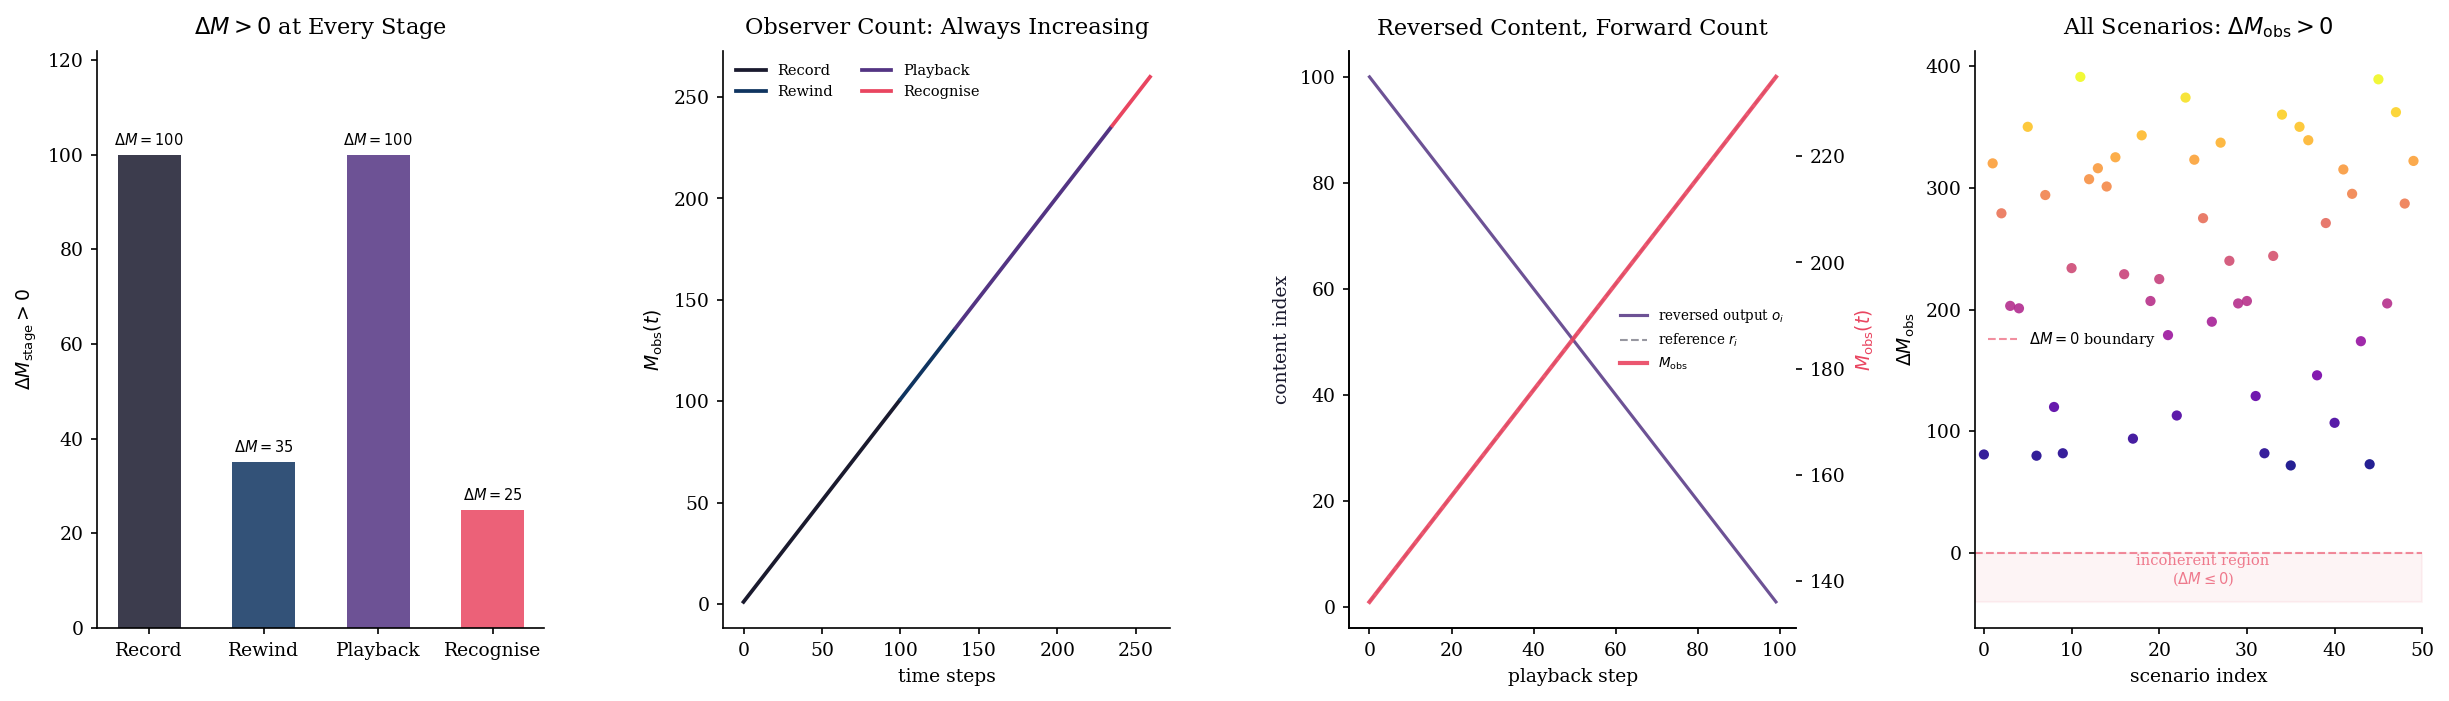
\includegraphics[width=\textwidth]{panels/panel_08_observer_forward_direction.png}
    \caption{\textbf{Every component of any apparent time-reversal scenario---production,
    mediation, and observation---is a forward partition event with $\Delta M > 0$;
    the temporal inversion is a property of output encoding, not of any partition count
    (Theorems~\ref{thm:forward-all} and~\ref{thm:obs-recognition};
    Remark~\ref{rem:cassette}).}
    (\textbf{A})~The cassette tape scenario decomposed into four stages (Record, Rewind,
    Playback, Recognise), with $\Delta M > 0$ annotated at each stage.  No stage has
    $\Delta M \leq 0$; the ``reversal'' lives entirely in the content-ordering of the
    output, not in the direction of any partition count.
    (\textbf{B})~The observer's cumulative count $M_{\mathrm{obs}}(t)$ across all four
    stages, coloured by stage.  The count is strictly monotone throughout: the observer
    advances forward in partition time during every phase of the observation, including
    the phase in which the reversed output is being perceived.
    (\textbf{C})~Reference sequence $\{r_i\}$ (dashed) and reversed output $\{o_i =
    r_{k+1-i}\}$ (solid) during playback (left axis), overlaid with
    $M_{\mathrm{obs}}(t)$ (right axis).  Content is in reverse order; the observer's
    partition count advances forward simultaneously.  The two axes are independent:
    content ordering and partition direction are separate predicates with no mutual
    implication.
    (\textbf{D})~For $50$ independent apparent-reversal scenarios, $\Delta M_{\mathrm{obs}} > 0$
    in every case, coloured by duration (plasma scale).  All points lie strictly above
    the $\Delta M = 0$ boundary (dashed); the incoherent region ($\Delta M \leq 0$)
    is shaded below.  No scenario witnesses or instantiates a backward partition event.}%
    \label{fig:panel8_observer_forward_direction}
\end{figure*}

% ──────────────────────────────────────────────────────────────────────────────
\begin{figure*}[!htbp]
    \centering
    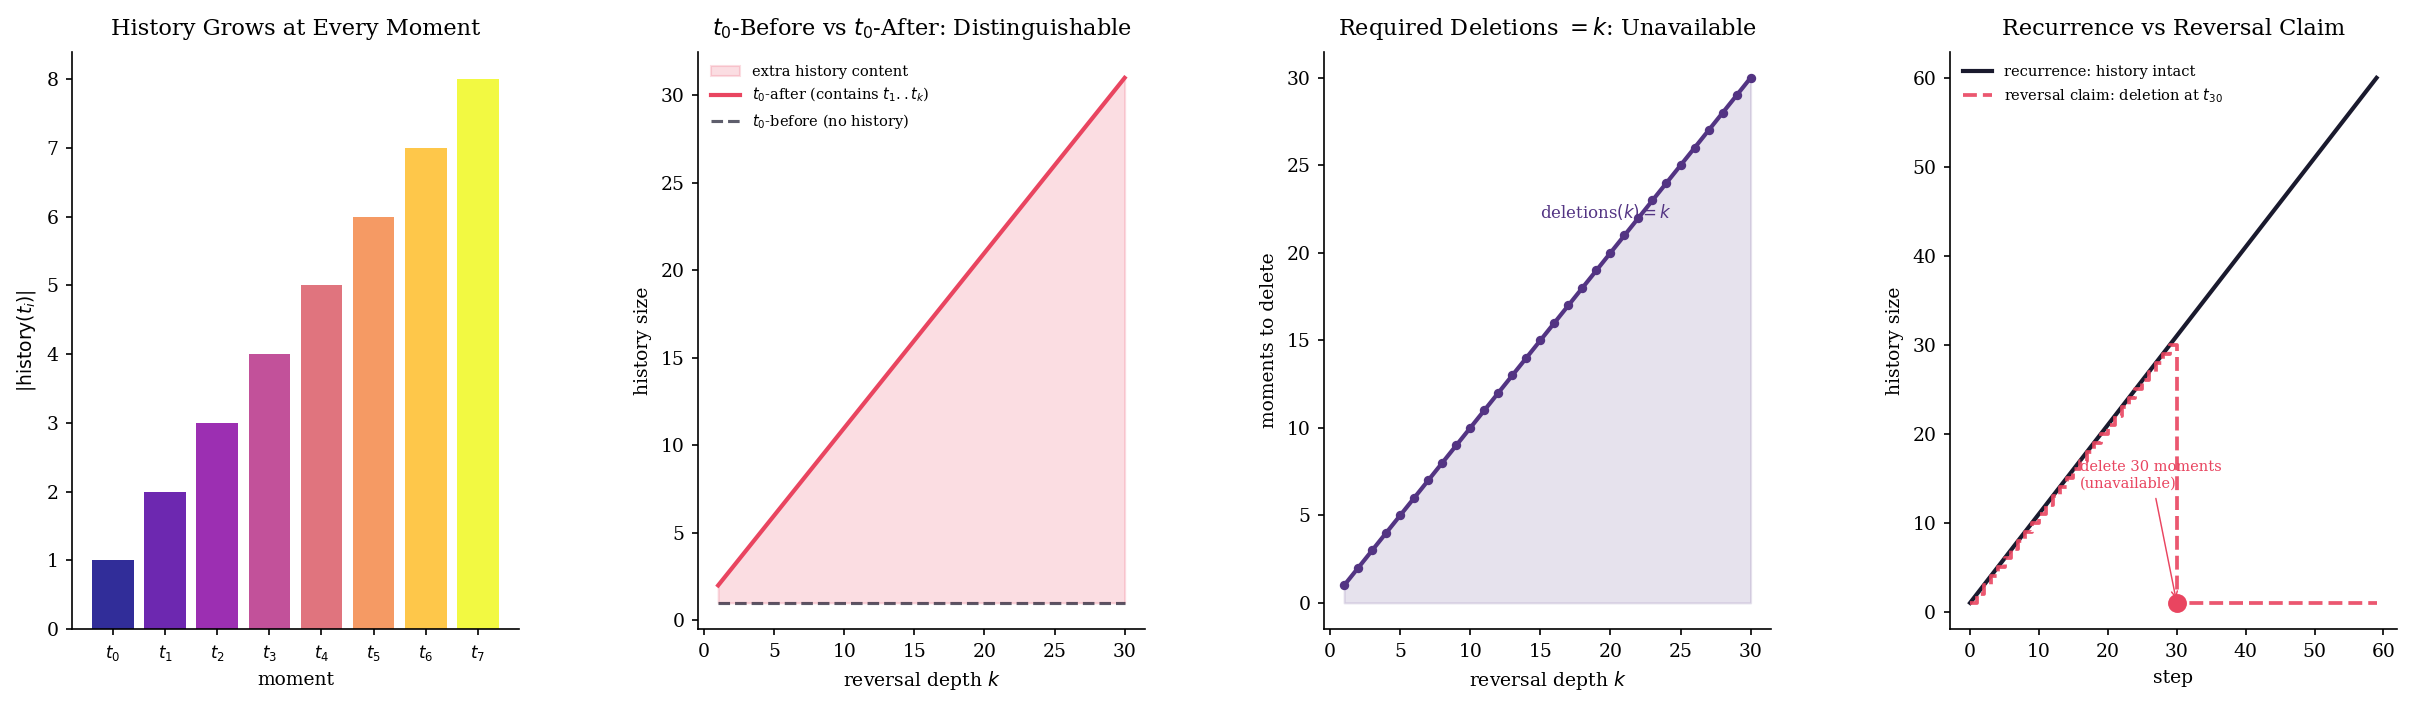
\includegraphics[width=\textwidth]{panels/panel_09_history_deletion.png}
    \caption{\textbf{Genuine time reversal from $t_k$ to $t_0$ requires deleting the
    intervening moments $t_1,\ldots,t_{k-1}$ from the universe's history; the required
    deletions grow linearly with reversal depth, and deletion is not an available
    physical operation
    (Theorems~\ref{thm:deletion} and~\ref{thm:no-deletion};
    Definition~\ref{def:distinguishability}).}
    (\textbf{A})~History size at each moment $t_i$: $|\mathrm{history}(t_i)| = i+1$,
    coloured by moment index (plasma scale).  History grows monotonically; no physical
    process reduces it.  The state at any moment includes the full causal record of all
    prior moments (Definition~\ref{def:distinguishability}).
    (\textbf{B})~State at $t_0$-before (history size $= 1$, dashed) versus state at
    $t_0$-after-reversal from depth $k$ (history size $= k+1$, solid), with shaded
    extra content.  The two states are distinguishable by their histories and are
    therefore distinct.  For the reversal claim to hold, the $k$ extra moments must be
    absent from the post-reversal state.
    (\textbf{C})~Required deletions as a function of reversal depth $k$:
    deletions$(k) = k$ exactly, growing linearly (shaded fill).  Any reversal of
    depth $k \geq 1$ requires at least one deletion; deletion is structurally
    unavailable (Theorem~\ref{thm:no-deletion}).
    (\textbf{D})~Recurrence (solid): history grows as the system evolves forward;
    at the recurrence step the configuration matches $t_0$ but the history is intact.
    Reversal claim (dashed): history would need to snap back to size $1$ at step $30$,
    requiring deletion of $30$ moments.  The sharp discontinuity marks the deletion
    event; no physical process produces it.  This panel directly visualises the
    distinction between recurrence and reversal established by
    Corollary~\ref{cor:egg-cycle}.}%
    \label{fig:panel9_history_deletion}
\end{figure*}

% ──────────────────────────────────────────────────────────────────────────────
\begin{figure*}[!htbp]
    \centering
    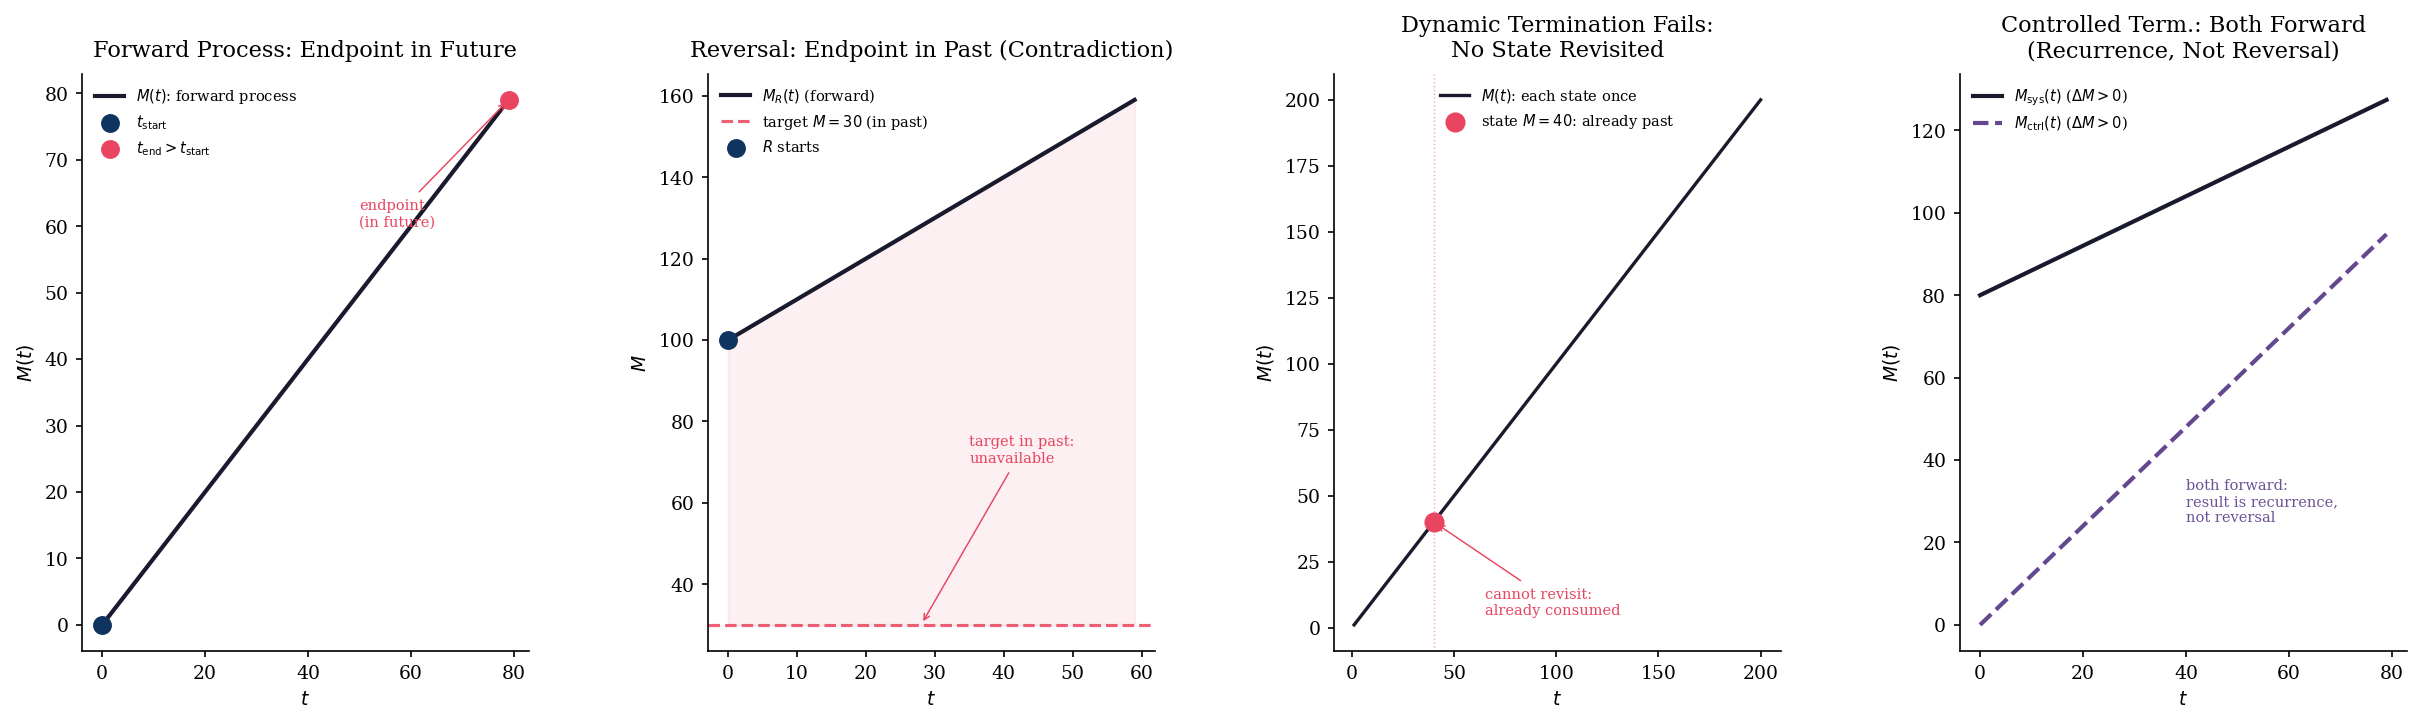
\includegraphics[width=\textwidth]{panels/panel_10_process_termination.png}
    \caption{\textbf{A reversal process $R$ has no available termination structure:
    its endpoint is a past state unreachable by dynamic termination
    (Corollary~\ref{cor:no-repeat}), and controlled termination collapses the reversal
    claim into a forward-time recurrence; no third mechanism exists
    (Theorem~\ref{thm:reversal-no-process}; Definition~\ref{def:process}).}
    (\textbf{A})~A forward process: $M(t)$ increases from $t_{\mathrm{start}}$ (blue) to
    $t_{\mathrm{end}}$ (orange).  The endpoint lies in the process's future; the
    forward dynamics determine when it is reached.  This is the canonical structure
    of any process in the sense of Definition~\ref{def:process}.
    (\textbf{B})~Putative reversal process $R$: $M_R(t)$ increases from $M = 100$ onward
    (forward time), but the target endpoint is the past state at $M = 30$ (dashed
    horizontal).  The gap between $M_R(t)$ and the target grows monotonically;
    dynamic termination cannot close this gap because the target recedes as $R$
    advances.
    (\textbf{C})~Dynamic termination fails: each partition state is visited exactly once
    along the forward trajectory (Corollary~\ref{cor:no-repeat}).  The state at
    $M = 40$ (orange marker) was consumed at step $40$ and cannot be revisited; a
    ``return'' requires a second visit, which the injectivity of $\Phi$ excludes.
    (\textbf{D})~Controlled termination yields recurrence, not reversal: both
    $M_{\mathrm{sys}}(t)$ (solid) and $M_{\mathrm{ctrl}}(t)$ (dashed) are strictly
    increasing.  The controller uses memory of a past configuration to navigate the
    system to a resembling configuration; both agents run forward.  This is a
    forward-time memory-driven recurrence of the kind formalised in
    Corollary~\ref{cor:egg-cycle}, not genuine reversal.}%
    \label{fig:panel10_process_termination}
\end{figure*}

% after the figures are placed in the manuscript.

% ──────────────────────────────────────────────────────────────────────────────
\begin{figure*}[!htbp]
    \centering
    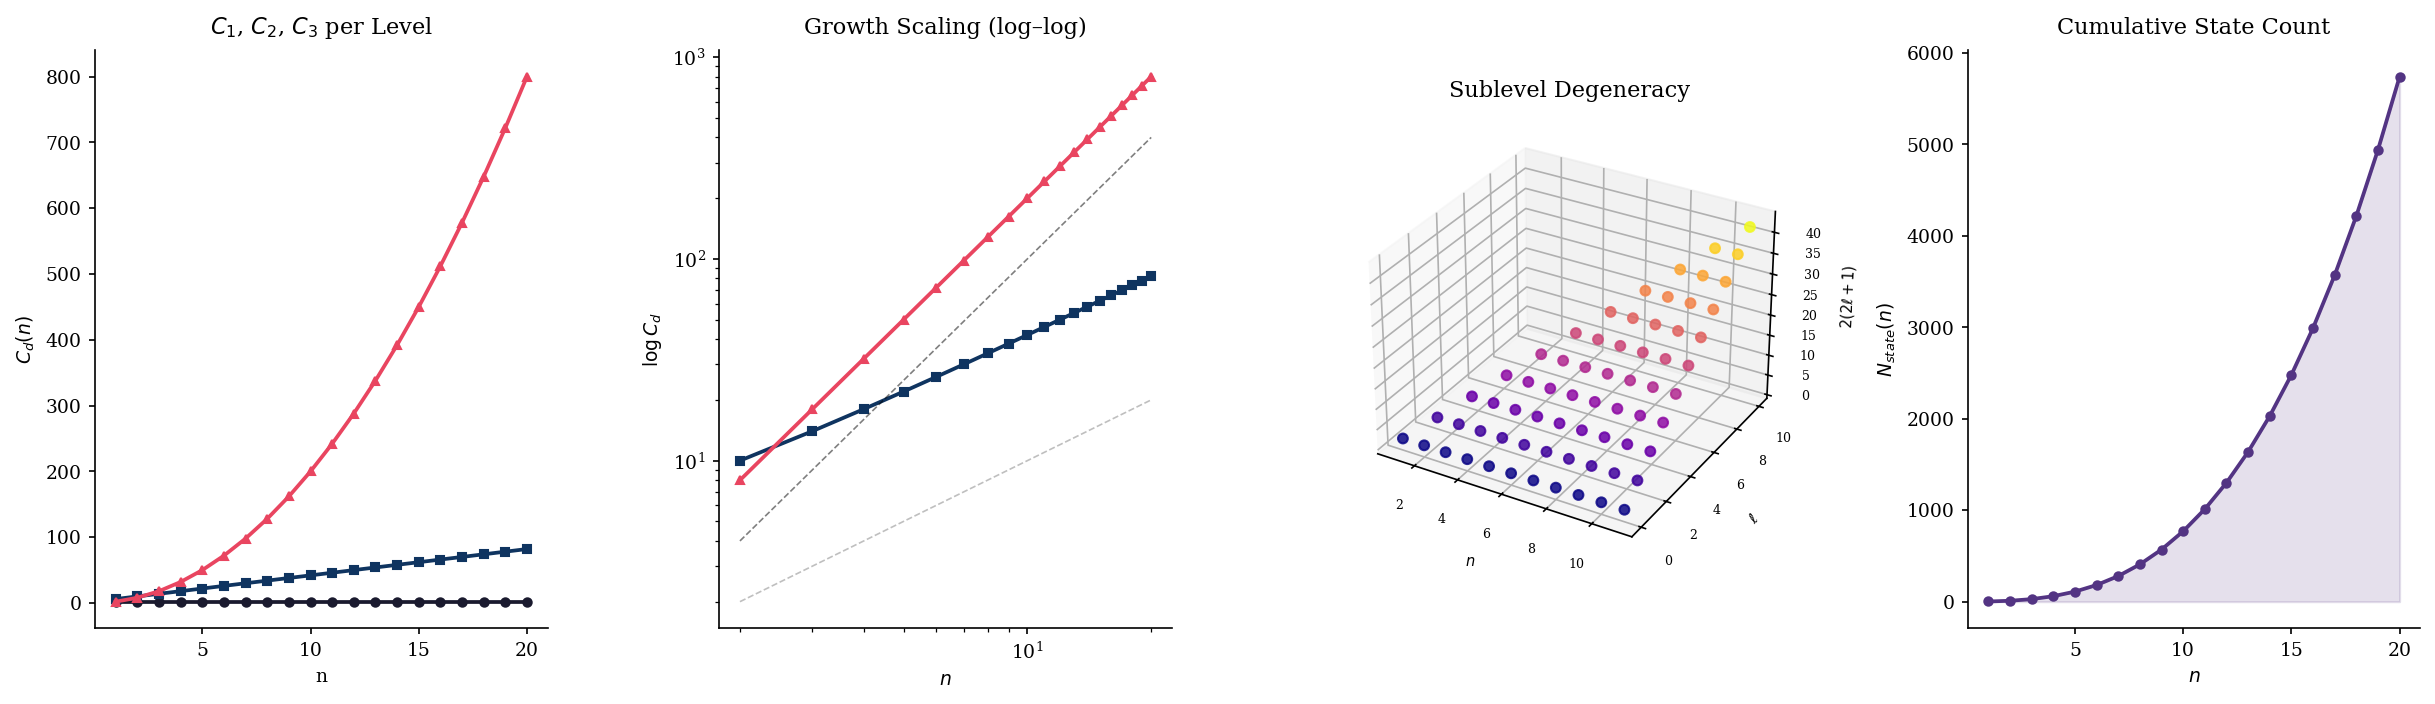
\includegraphics[width=\textwidth]{panels/panel_01_capacity_hierarchy.png}
    \caption{\textbf{Capacity growth $C_d(n)$ is constant in $d{=}1$, linear in $d{=}2$, and
    quadratic in $d{=}3$, establishing a strict dimensional hierarchy whose slope on a
    log–log axis discriminates the angular dimension of each within-level partition space
    (Definition~\ref{def:cap-d}; Theorem~\ref{thm:capacity}).}
    (\textbf{A})~Line plot of per-level capacity $C_d(n)$ versus principal quantum number $n$
    for $d{=}1$ (dark, flat), $d{=}2$ (mid, linear), and $d{=}3$ (light, quadratic).
    The three curves separate immediately at $n{=}2$: $C_1$ remains fixed at $2$; $C_2$
    grows as $4n{+}2$; $C_3 = 2n^2$ accelerates away from both, reflecting the
    two-dimensional angular structure of the within-level space $L_n^{(3)}$.
    (\textbf{B})~Log–log plot of $C_2(n)$ and $C_3(n)$ for $n \geq 3$, overlaid with reference
    lines of slope $1$ (linear, grey dashed) and slope $2$ (quadratic, black dashed).
    $C_2$ tracks the slope-$1$ reference exactly; $C_3$ tracks slope $2$ exactly,
    confirming that the exponent of capacity growth equals the continuous angular
    dimension of $L_n^{(d)}$: $0$ for $d{=}1$, $1$ for $d{=}2$, $2$ for $d{=}3$.
    (\textbf{C})~Three-dimensional scatter of sublevel degeneracy $2(2\ell+1)$ plotted against
    principal level $n$ (x-axis) and angular index $\ell$ (y-axis) for $n = 1,\ldots,11$.
    Colour encodes degeneracy magnitude (plasma scale).  The surface rises along both
    axes, with the steepest growth in $\ell$ at fixed $n$, reproducing the quadratic
    capacity as $C_3(n) = \sum_{\ell=0}^{n-1} 2(2\ell{+}1)$.
    (\textbf{D})~Line plot of cumulative state count $N_\mathrm{state}(n) = n(n{+}1)(2n{+}1)/3$
    versus $n$ with shaded fill.  The cubic growth follows directly from summing the
    quadratic per-level capacity; the steepening curvature is the algebraic signature
    that each added level contributes an accelerating number of partition states, as
    stated in Corollary~\ref{cor:cumulative}.}%
    \label{fig:panel1_capacity_hierarchy}
\end{figure*}

% ──────────────────────────────────────────────────────────────────────────────
\begin{figure*}[!htbp]
    \centering
    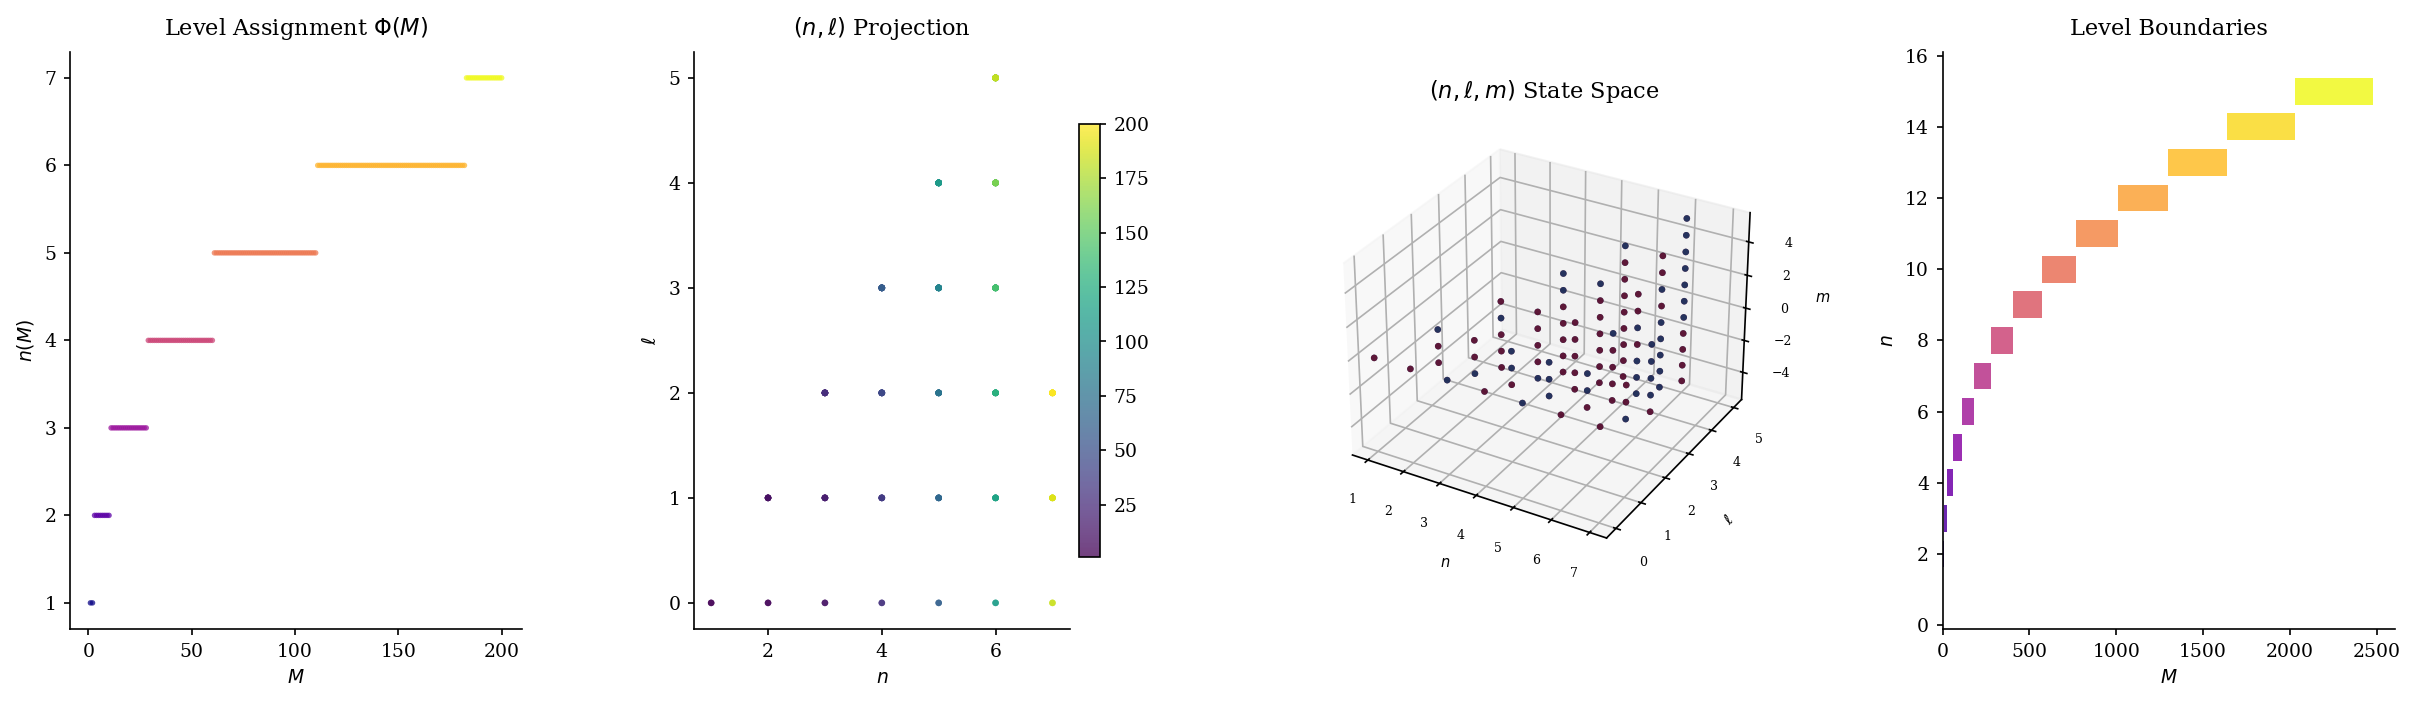
\includegraphics[width=\textwidth]{panels/panel_02_bijection_structure.png}
    \caption{\textbf{The partition map $\Phi:\mathbb{Z}^{+}\!\to\mathcal{P}$ is a
    well-defined bijection whose image tiles three-dimensional quantum-number space
    without collision or gap, and whose level boundaries are sharp staircase
    transitions determined by the cumulative capacity formula
    (Theorem~\ref{thm:bijection}; Corollary~\ref{cor:cumulative}).}
    (\textbf{A})~Scatter of principal level $n(\Phi(M))$ versus integer index $M$ for
    $M = 1,\ldots,200$, coloured by $n$ (plasma scale).  Level transitions appear as
    discrete upward steps; within each band $M$ increments uniformly, confirming
    that $\Phi$ exhausts every state of level $n$ before advancing to $n{+}1$.
    (\textbf{B})~Two-dimensional projection onto the $(n,\ell)$ plane, coloured by $M$
    (viridis scale).  Each point $(n,\ell)$ appears with multiplicity $2(2\ell{+}1)$,
    one for each $(m,s)$ pair; the colour gradient shows that $M$ increases
    monotonically left-to-right and bottom-to-top within each level, establishing
    the lexicographic ordering of $\Phi$.
    (\textbf{C})~Three-dimensional scatter of the full quantum-number triple $(n,\ell,m)$
    for $M = 1,\ldots,200$, with colour encoding spin $s = \pm\tfrac{1}{2}$ (red–blue
    diverging scale).  The cloud fills a triangular prism in $(n,\ell,m)$ space:
    $0 \leq \ell \leq n{-}1$, $-\ell \leq m \leq \ell$.  No two points coincide,
    providing visual confirmation of injectivity (Theorem~\ref{thm:bijection}).
    (\textbf{D})~Horizontal bar chart of level sizes: each bar spans the $M$-range
    $[N_\mathrm{state}(n{-}1){+}1,\, N_\mathrm{state}(n)]$ for levels $n = 1,\ldots,15$,
    coloured by level index.  Bar widths equal $C_3(n) = 2n^2$, growing quadratically;
    the staircase of left boundaries locates the exact $M$-index at which each new
    principal level begins, as derived in Corollary~\ref{cor:cumulative}.}%
    \label{fig:panel2_bijection_structure}
\end{figure*}

% ──────────────────────────────────────────────────────────────────────────────
\begin{figure*}[!htbp]
    \centering
    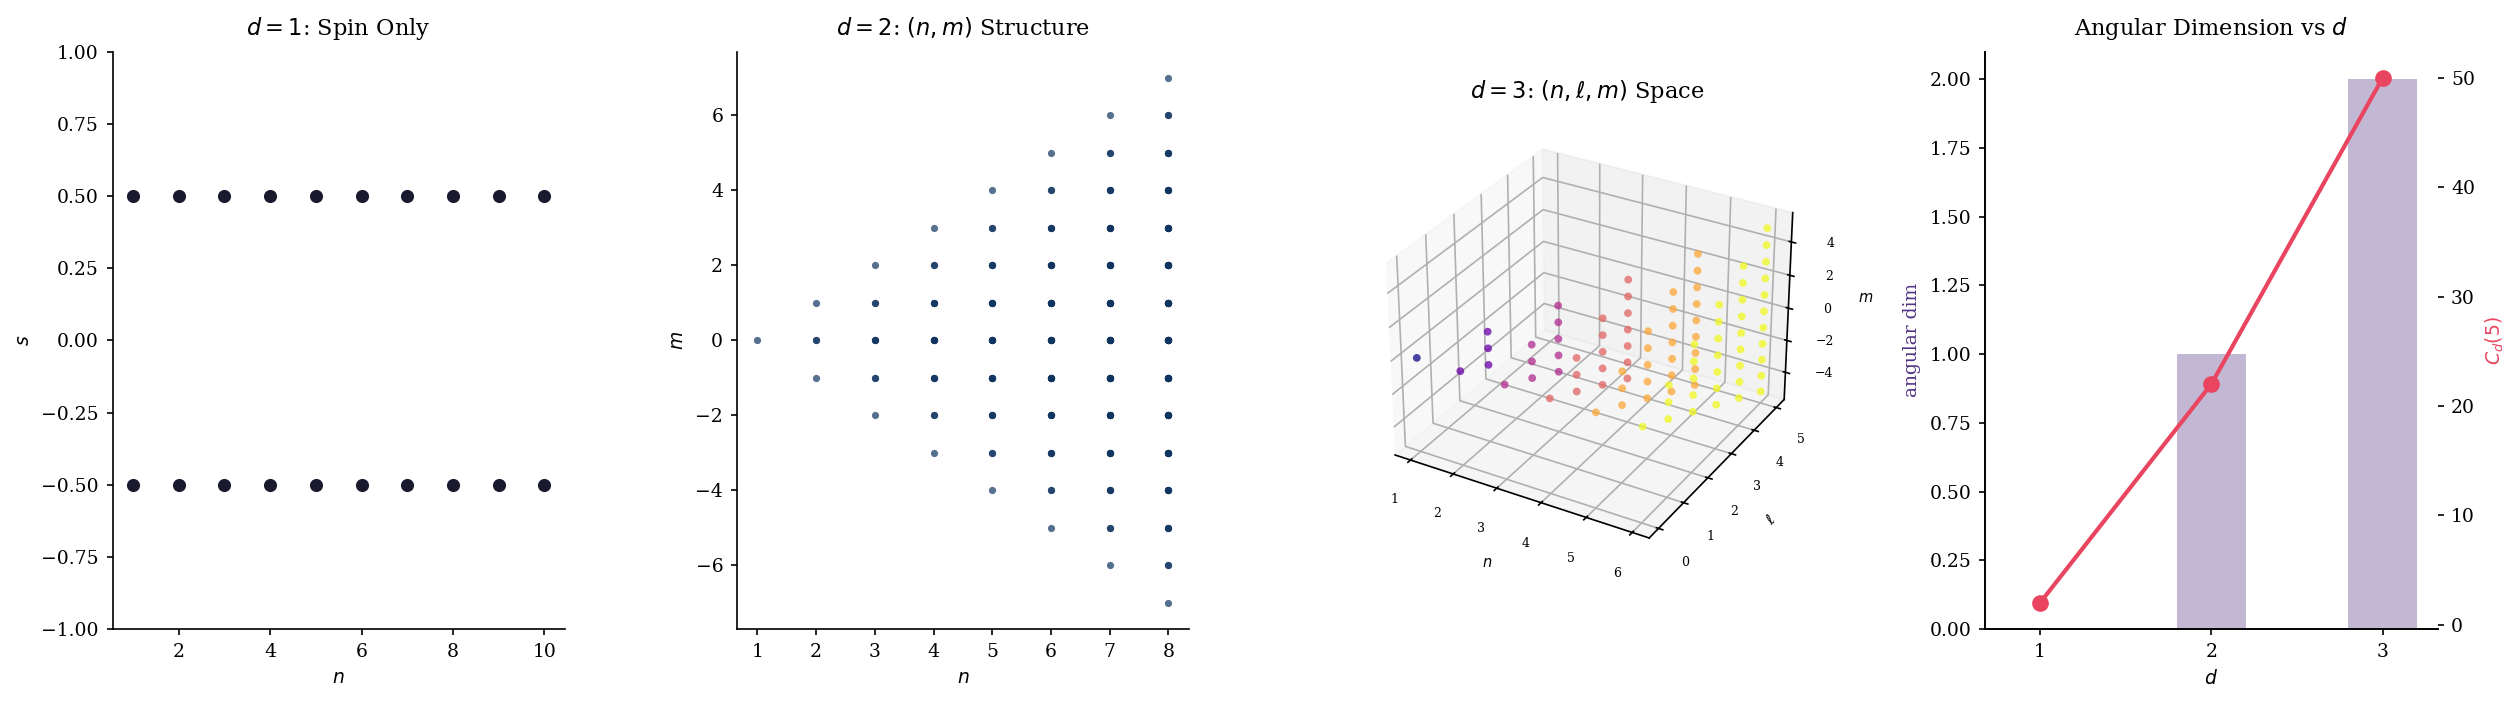
\includegraphics[width=\textwidth]{panels/panel_03_partition_geometry.png}
    \caption{\textbf{Spatial dimension $d{=}3$ is the minimum for which the within-level
    partition space $L_n^{(d)}$ has continuous angular dimension $\geq 2$, enabling
    negation to close around any state from all angular directions simultaneously
    (Theorem~\ref{thm:min-dim}; Definition~\ref{def:within-level}).}
    (\textbf{A})~Scatter of partition states in $d{=}1$: only the spin coordinate $s =
    \pm\tfrac{1}{2}$ varies; every level $n$ contributes exactly two isolated points.
    The within-level space $L_n^{(1)}$ has angular dimension $0$: there is no
    continuous angular degree of freedom, so negation from the ``left'' and ``right''
    cannot simultaneously enclose the state.
    (\textbf{B})~Scatter of partition states $(n, m)$ for $d{=}2$, $n = 1,\ldots,8$.
    Within level $n$, the $m$-values $\{-(n{-}1),\ldots,n{-}1\}$ form a one-dimensional
    chain; $L_n^{(2)}$ has angular dimension $1$.  Two opposing states can bracket any
    given $m$, but the within-level topology is a line segment, not a closed surface,
    so negation-closure is incomplete.
    (\textbf{C})~Three-dimensional scatter of partition states $(n, \ell, m)$ for $d{=}3$,
    $n = 1,\ldots,6$, coloured by $n$ (plasma scale).  Within level $n$, the pairs
    $(\ell, m)$ fill a two-dimensional triangular region; $L_n^{(3)}$ has angular
    dimension $2$.  Every interior point is enclosed from all angular directions,
    satisfying the closure condition of Theorem~\ref{thm:min-dim}.
    (\textbf{D})~Combined bar and line chart comparing angular dimension (left axis, bars)
    and per-level capacity $C_d(5)$ (right axis, line with markers) for $d = 1, 2, 3$.
    Angular dimension steps $0 \to 1 \to 2$ in exact correspondence with the
    exponent governing $C_d$, confirming that the quadratic capacity of $d{=}3$ is the
    algebraic signature of the minimum dimensionality required for
    negation-constituted closure.}%
    \label{fig:panel3_partition_geometry}
\end{figure*}

% ──────────────────────────────────────────────────────────────────────────────
\begin{figure*}[!htbp]
    \centering
    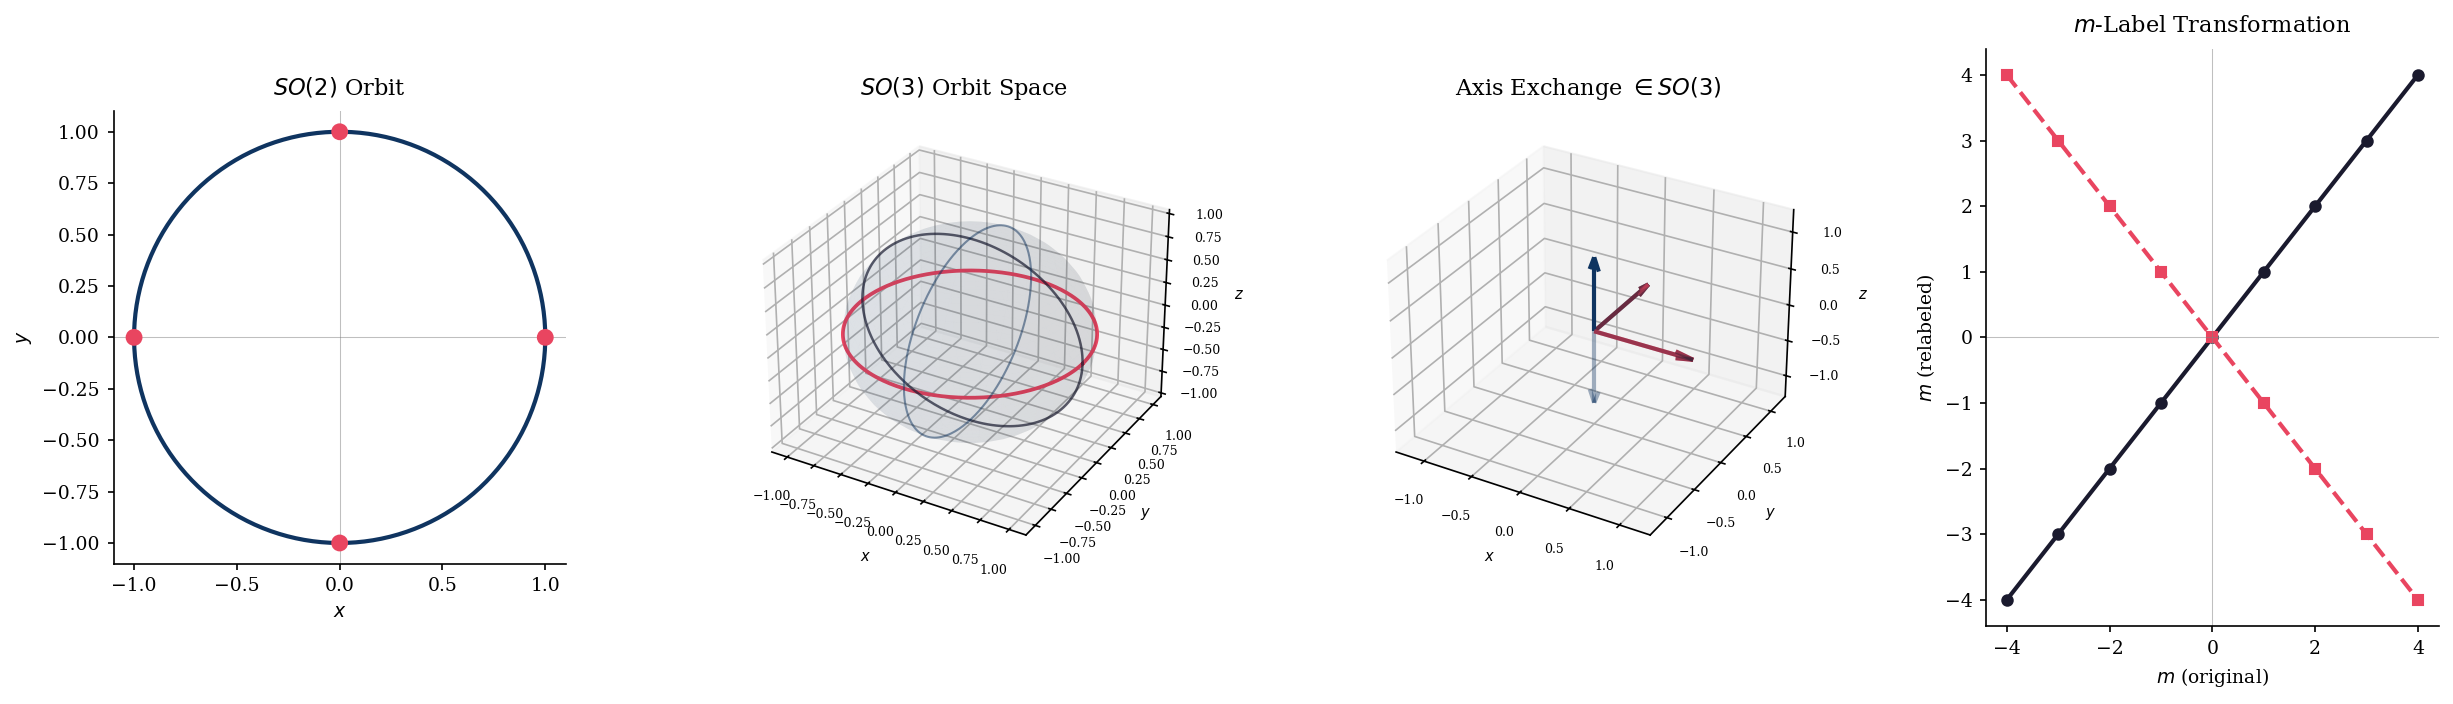
\includegraphics[width=\textwidth]{panels/panel_04_SO3_symmetry.png}
    \caption{\textbf{The axis exchange $(x,y,z)\mapsto(y,x,-z)$ is a proper rotation
    in $SO(3)$ with $\det = +1$, but the analogous swap $x \leftrightarrow y$ in
    $d{=}2$ is an improper reflection with $\det = -1$; consequently, the
    $m$-label is $SO(2)$-invariant but changes under $SO(3)$ axis relabelling,
    and partition identity is reference-frame-independent only for $d\geq 3$
    (Corollary~\ref{cor:axis-exchange}).}
    (\textbf{A})~$SO(2)$ orbit: unit circle in the $xy$-plane with four marked points at
    $(\pm 1, 0)$ and $(0, \pm 1)$.  All rotations in $SO(2)$ preserve orientation;
    the swap $x \leftrightarrow y$ in two dimensions corresponds to reflection
    across the diagonal, an element of $O(2) \setminus SO(2)$ with $\det = -1$.
    (\textbf{B})~$SO(3)$ orbit space: transparent unit sphere with equatorial orbit
    (coloured ring, equator plane) and two meridional great-circle orbits.  The full
    $SO(3)$ orbit of a fixed axis direction sweeps a two-sphere, capturing the
    additional degree of freedom absent in $d{=}2$.
    (\textbf{C})~Three-dimensional axis-frame diagram visualising the exchange
    $R: (x,y,z)\mapsto(y,x,-z)$.  Solid arrows show the original frame
    $(\hat{e}_x, \hat{e}_y, \hat{e}_z)$; translucent arrows show the relabelled
    frame.  This transformation lies in $SO(3)$ ($\det R = +1$, angle $=\pi$ about
    the axis $\frac{1}{\sqrt{2}}(\hat{e}_x + \hat{e}_y)$), making it a physically
    accessible change of reference frame rather than an orientation reversal.
    (\textbf{D})~Line plot of the $m$-label transformation for $\ell = 4$ under the two
    symmetry groups.  Under $SO(2)$ rotation about $\hat{z}$, the eigenvalue $m$
    is invariant (identity line, dark).  Under the $SO(3)$ axis exchange of panel
    (C), $L_z \to -L_z$ and $m \mapsto -m$ (reflected line, light).  The
    non-trivial relabelling confirms that $m$ encodes a reference-frame choice,
    not an observer-independent integer, whenever $d \geq 3$.}%
    \label{fig:panel4_SO3_symmetry}
\end{figure*}

% ──────────────────────────────────────────────────────────────────────────────
\begin{figure*}[!htbp]
    \centering
    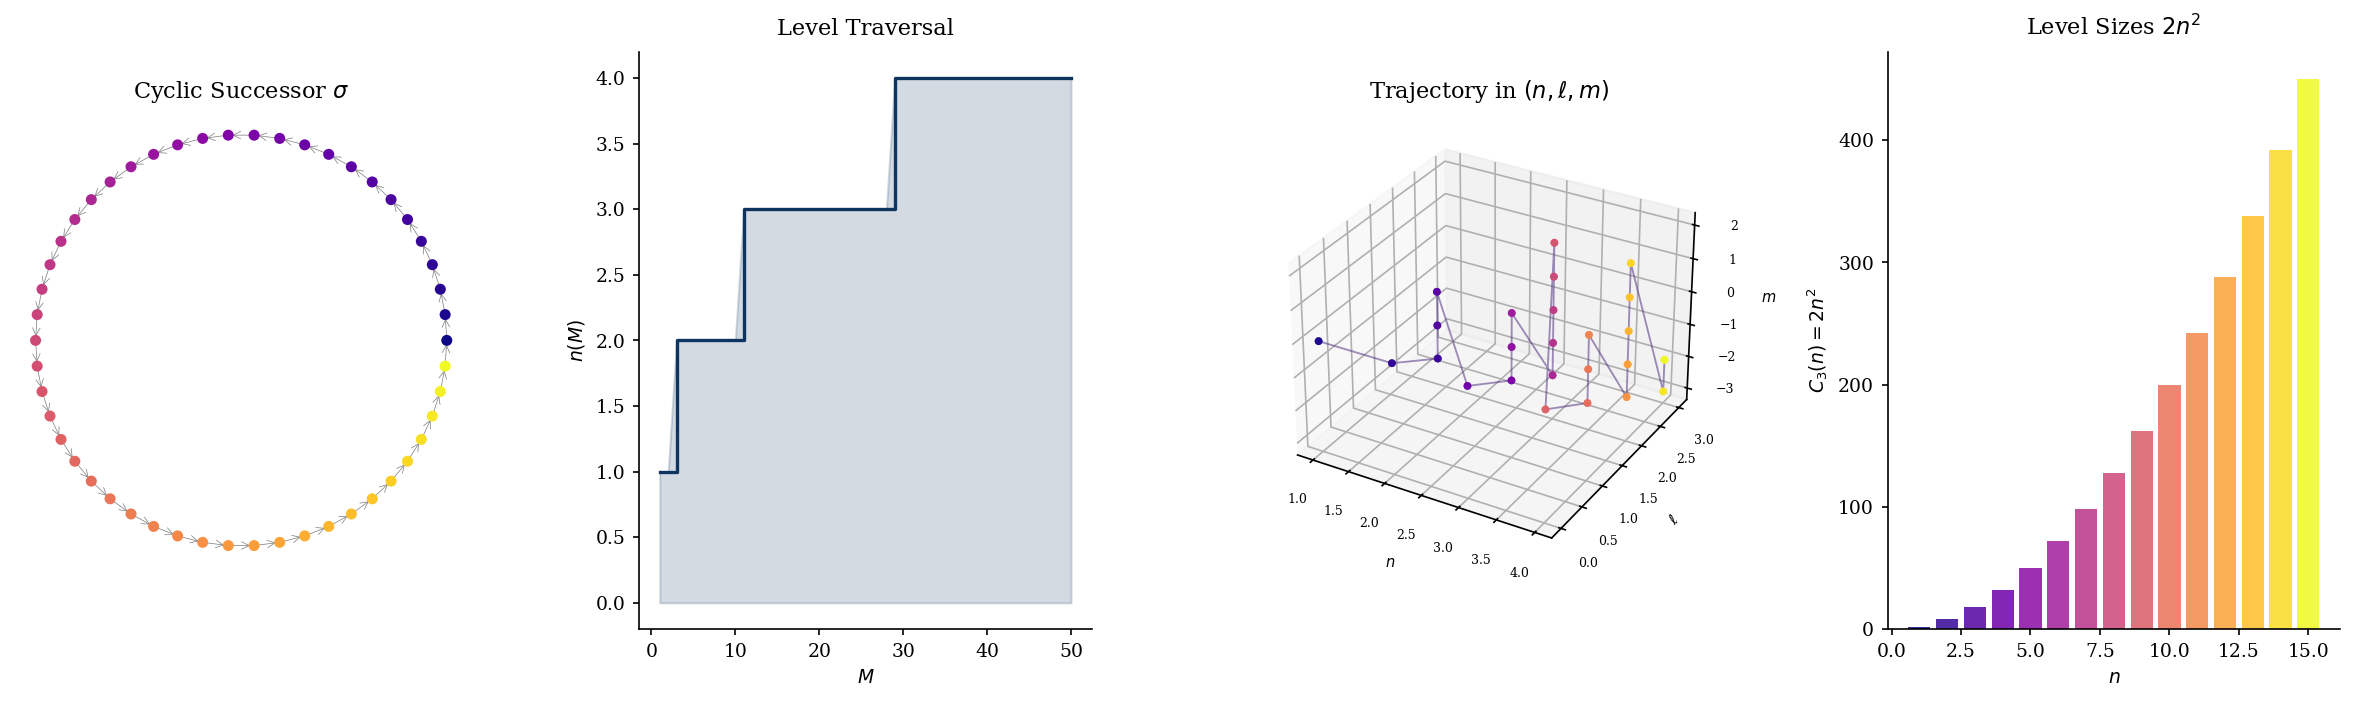
\includegraphics[width=\textwidth]{panels/panel_05_cyclic_closure.png}
    \caption{\textbf{The successor relation $\sigma$ is a bijection on the finite partition
    category $\mathcal{C}$ whose unique cycle has length $M_{\max} = N_\mathrm{state}(n_{\max})$,
    forcing every state—including $\Phi(1)$—to be revisited exactly once per period and
    making cyclic closure a structural consequence of finiteness rather than a dynamical
    assumption (Theorem~\ref{thm:cyclic}; Theorem~\ref{thm:cat-closure}).}
    (\textbf{A})~Cyclic successor diagram for $M_{\max} = 50$: each partition state is
    placed on a unit circle at angle $2\pi M / M_{\max}$, coloured by $M$ (plasma
    scale), with grey arrows connecting $\Phi(M)$ to $\sigma(\Phi(M)) = \Phi(M{+}1)$.
    The final arrow from $\Phi(50)$ returns to $\Phi(1)$, completing the cycle and
    confirming that $\sigma$ is a permutation of $\mathcal{C}$ with no fixed points
    and no proper sub-cycles (Theorem~\ref{thm:cyclic}).
    (\textbf{B})~Step plot of the level assignment $n(M)$ for $M = 1,\ldots,50$, with
    shaded fill below the curve.  Each plateau spans exactly $C_3(n) = 2n^2$ consecutive
    integers; the risers are instantaneous, reflecting the sharp level boundary at
    $M = N_\mathrm{state}(n)$.  The sequence is strictly non-decreasing (Theorem~\ref{thm:monotone}),
    encoding the irreversibility of temporal progression within the bijective ordering.
    (\textbf{C})~Three-dimensional trajectory through $(n, \ell, m)$ state space for
    $M = 1,\ldots,50$, with points coloured by $M$ (plasma scale) and connected by a
    curve.  The path climbs through successive levels, executes a zig-zag pattern
    within each level as $\ell$ and $m$ increment lexicographically, then returns to
    the origin upon cyclic closure.  The trajectory is injective on any open arc but
    closed as a whole (Corollary~\ref{cor:cyclic}).
    (\textbf{D})~Bar chart of level sizes $C_3(n) = 2n^2$ for $n = 1,\ldots,15$, coloured
    by level index.  Quadratic growth of bar height reflects the quadratic capacity law;
    the total area equals $M_{\max} = N_\mathrm{state}(n_{\max})$, the unique cycle length.
    The accelerating size of successive levels means that higher-$n$ states are
    structurally ``harder to reach'' in the sense of requiring a longer prefix of
    the successor sequence.}%
    \label{fig:panel5_cyclic_closure}
\end{figure*}

% ──────────────────────────────────────────────────────────────────────────────
\begin{figure*}[!htbp]
    \centering
    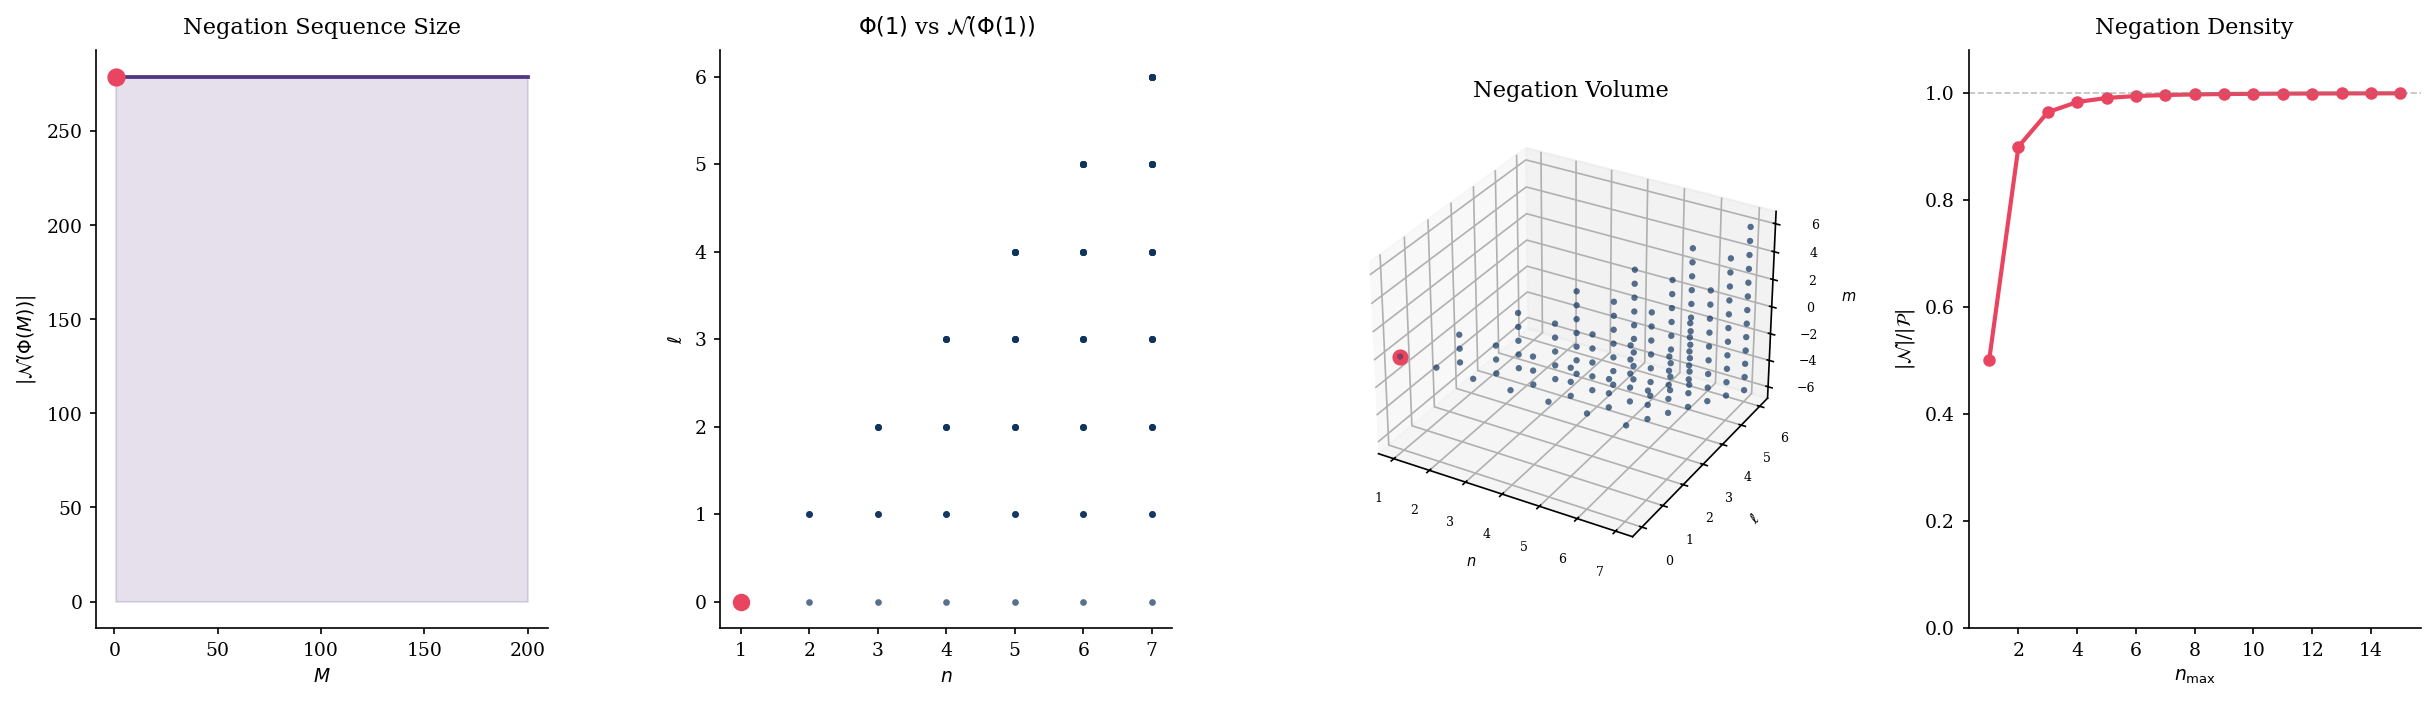
\includegraphics[width=\textwidth]{panels/panel_06_negation_identity.png}
    \caption{\textbf{Every partition state $\Phi(M)$ is uniquely identified by its negation
    sequence $\mathcal{N}(\Phi(M)) = \mathcal{P} \setminus \{\Phi(M)\}$, and the ground
    state $\Phi(1) = (1,0,0,+\tfrac{1}{2})$ possesses the largest possible negation
    sequence while being categorically irreducible, making it the structurally necessary
    origin of the partition sequence
    (Theorem~\ref{thm:negation-duality}; Definition~\ref{def:ground-cat};
    Theorem~\ref{thm:sing-necessity}).}
    (\textbf{A})~Scatter and fill of $|\mathcal{N}(\Phi(M))| = |\mathcal{P}| - 1$ versus $M$
    for $M = 1,\ldots,200$.  The value is constant across all $M$: every state has
    exactly one fewer element in its negation sequence than the cardinality of
    $\mathcal{P}$, because negation excludes only $\Phi(M)$ itself.  The ground state
    $\Phi(1)$ is marked (orange dot); it is distinguished not by a different negation
    size but by the property that $\Phi(1)$ has no $\sigma$-predecessor in
    $\mathcal{P}$ (Theorem~\ref{thm:sing-necessity}).
    (\textbf{B})~Two-dimensional scatter of the full partition space projected onto
    $(n, \ell)$ for $n = 1,\ldots,7$.  All states except $\Phi(1) = (1,0,0,+\tfrac{1}{2})$
    are shown in blue (the negation sequence $\mathcal{N}(\Phi(1))$); $\Phi(1)$ is marked
    in orange.  The visual contrast makes precise the duality $\mathcal{P} =
    \{\Phi(1)\} \cup \mathcal{N}(\Phi(1))$: identity is constituted by the totality
    of what it is not (Theorem~\ref{thm:negation-duality}).
    (\textbf{C})~Three-dimensional scatter of the full partition space in $(n, \ell, m)$
    for $n = 1,\ldots,7$.  Blue points form the negation volume $\mathcal{N}(\Phi(1))$;
    the single orange point at the origin $(1,0,0)$ is the ground state $\Phi(1)$.
    The geometric relationship captures the categorical claim: $\Phi(1)$ is the unique
    state maximally enclosed by its own negation set from all angular directions in
    the three-dimensional partition space.
    (\textbf{D})~Line plot of the negation density ratio $|\mathcal{N}| / |\mathcal{P}_{n_{\max}}|$
    versus the truncation level $n_{\max}$, where $|\mathcal{P}_{n_{\max}}| =
    N_\mathrm{state}(n_{\max})$.  The ratio $(N - 1)/N$ increases monotonically toward $1$
    as $n_{\max} \to \infty$, with the horizontal dashed line marking the asymptotic
    limit.  This convergence is the quantitative expression of the remark that any
    finite physical category saturates the negation relation: as the category grows,
    a state's identity becomes more fully determined by what it is not, with the
    ground state $\Phi(1)$ retaining the maximum negation complement at every
    finite truncation.}%
    \label{fig:panel6_negation_identity}
\end{figure*}

% ──────────────────────────────────────────────────────────────────────────────
\begin{figure*}[!htbp]
    \centering
    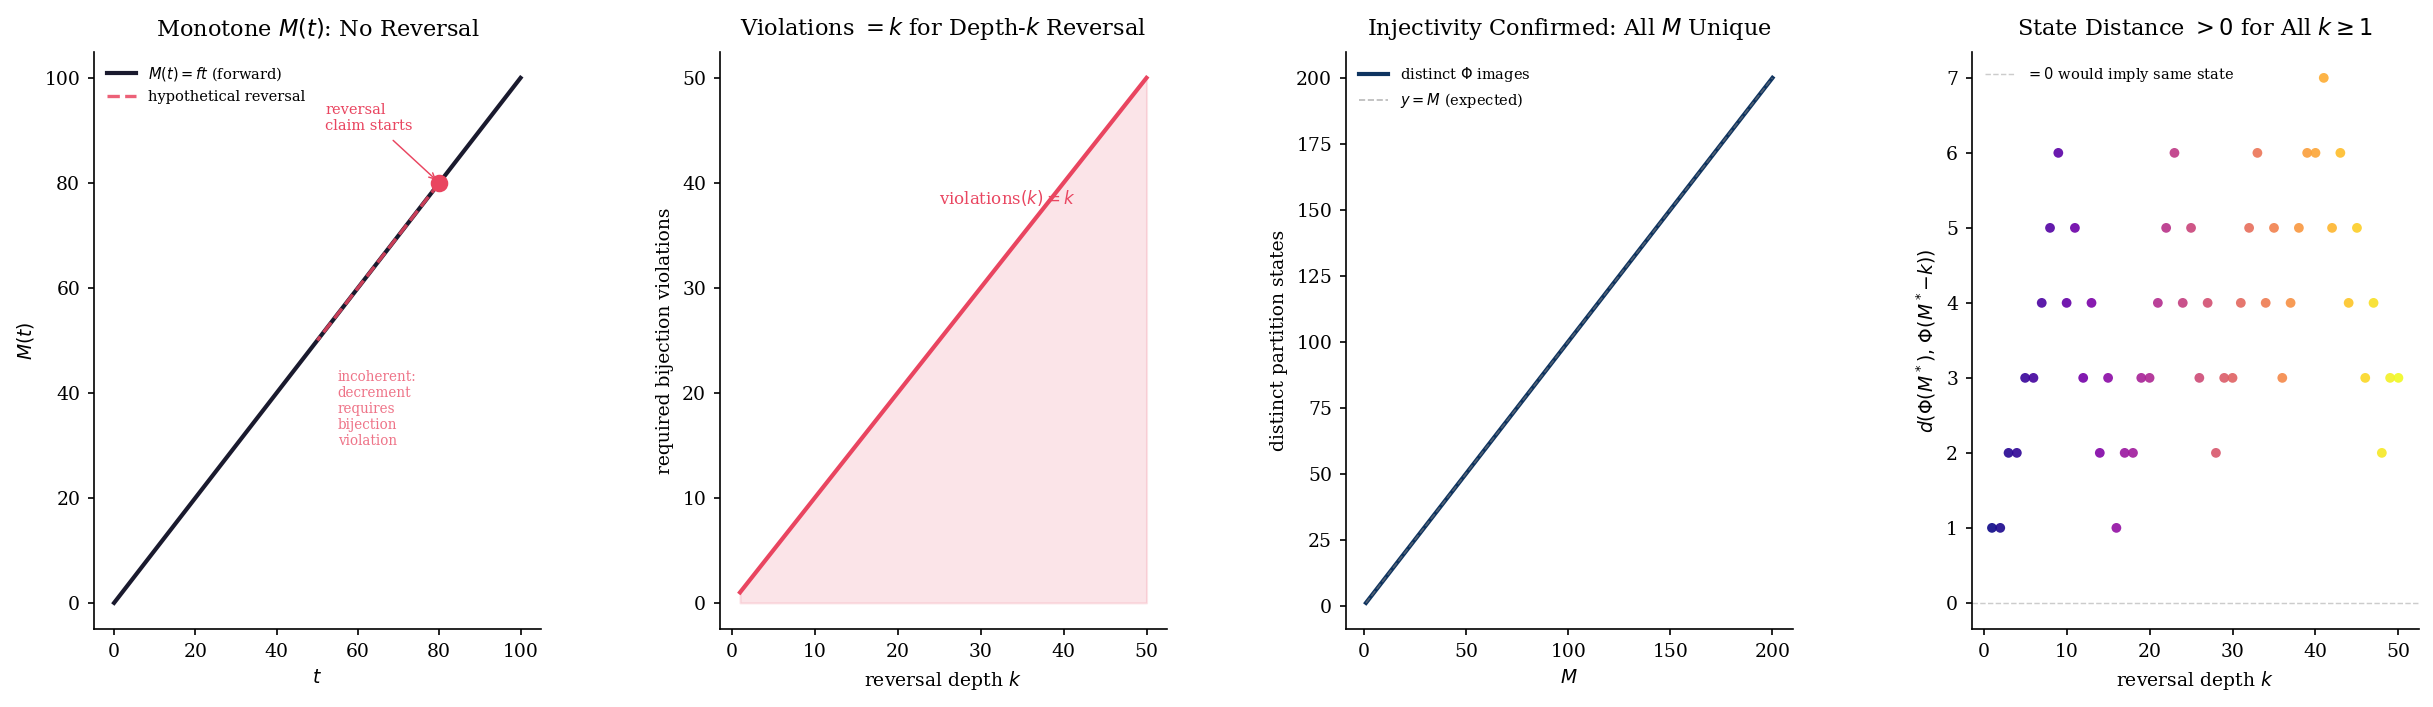
\includegraphics[width=\textwidth]{panels/panel_07_decrement_incoherence.png}
    \caption{\textbf{Any decrement $M \to M{-}k$ requires the bijection $\Phi$ to assign
    the same partition state to two distinct positive integers, violating injectivity;
    the number of required violations grows linearly with reversal depth $k$
    (Theorem~\ref{thm:incoherence}; Corollary~\ref{cor:loschmidt}).}
    (\textbf{A})~The partition count $M(t) = ft$ is strictly monotone (solid).  A
    hypothetical reversal segment (dashed, originating at $M = 80$) is shown; this
    trajectory has no physical realisation because no operation on the counting process
    corresponds to $\Delta M < 0$.
    (\textbf{B})~Required bijection violations as a function of reversal depth $k$,
    for a reversal originating at $M^{*} = 100$: violations$(k) = k$ exactly.  A
    depth-$k$ reversal forces $k$ distinct integers in $\Zp$ to share a single image
    under $\Phi$, contradicting Theorem~\ref{thm:bijection}.
    (\textbf{C})~Running count of distinct $\Phi$-images for $M = 1,\ldots,200$ (solid)
    overlaid on the identity line $y = M$ (dashed).  The two coincide exactly,
    confirming that all $200$ partition states are distinct and the bijection is
    injective with no collisions: the formal argument's central claim verified
    numerically at $M = 200$.
    (\textbf{D})~Manhattan distance $d(\Phi(M^{*}),\,\Phi(M^{*}{-}k))$ in partition-label
    space for $M^{*} = 100$, $k = 1,\ldots,50$, coloured by $k$ (plasma scale).
    Every distance is strictly positive: no two distinct integers share a
    partition-state image, confirming that any claimed decrement produces a genuine
    collision, not a near-miss.}%
    \label{fig:panel7_decrement_incoherence}
\end{figure*}

% ──────────────────────────────────────────────────────────────────────────────
\begin{figure*}[!htbp]
    \centering
    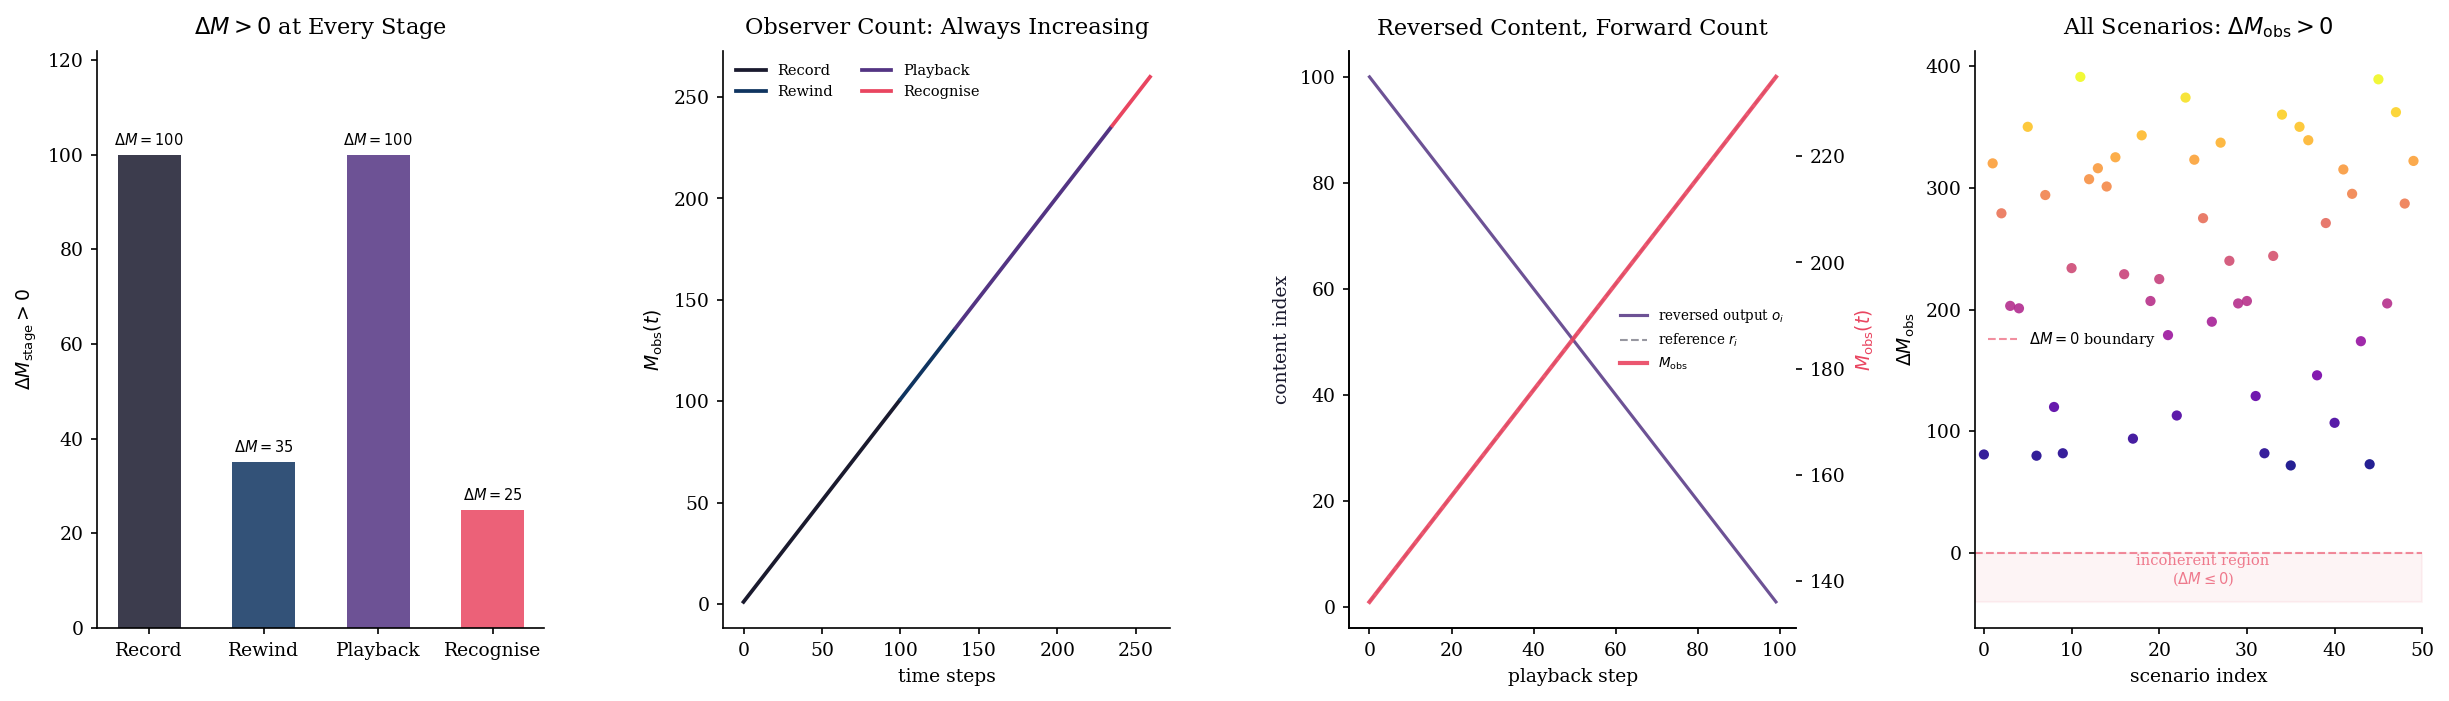
\includegraphics[width=\textwidth]{panels/panel_08_observer_forward_direction.png}
    \caption{\textbf{Every component of any apparent time-reversal scenario---production,
    mediation, and observation---is a forward partition event with $\Delta M > 0$;
    the temporal inversion is a property of output encoding, not of any partition count
    (Theorems~\ref{thm:forward-all} and~\ref{thm:obs-recognition};
    Remark~\ref{rem:cassette}).}
    (\textbf{A})~The cassette tape scenario decomposed into four stages (Record, Rewind,
    Playback, Recognise), with $\Delta M > 0$ annotated at each stage.  No stage has
    $\Delta M \leq 0$; the ``reversal'' lives entirely in the content-ordering of the
    output, not in the direction of any partition count.
    (\textbf{B})~The observer's cumulative count $M_{\mathrm{obs}}(t)$ across all four
    stages, coloured by stage.  The count is strictly monotone throughout: the observer
    advances forward in partition time during every phase of the observation, including
    the phase in which the reversed output is being perceived.
    (\textbf{C})~Reference sequence $\{r_i\}$ (dashed) and reversed output $\{o_i =
    r_{k+1-i}\}$ (solid) during playback (left axis), overlaid with
    $M_{\mathrm{obs}}(t)$ (right axis).  Content is in reverse order; the observer's
    partition count advances forward simultaneously.  The two axes are independent:
    content ordering and partition direction are separate predicates with no mutual
    implication.
    (\textbf{D})~For $50$ independent apparent-reversal scenarios, $\Delta M_{\mathrm{obs}} > 0$
    in every case, coloured by duration (plasma scale).  All points lie strictly above
    the $\Delta M = 0$ boundary (dashed); the incoherent region ($\Delta M \leq 0$)
    is shaded below.  No scenario witnesses or instantiates a backward partition event.}%
    \label{fig:panel8_observer_forward_direction}
\end{figure*}

% ──────────────────────────────────────────────────────────────────────────────
\begin{figure*}[!htbp]
    \centering
    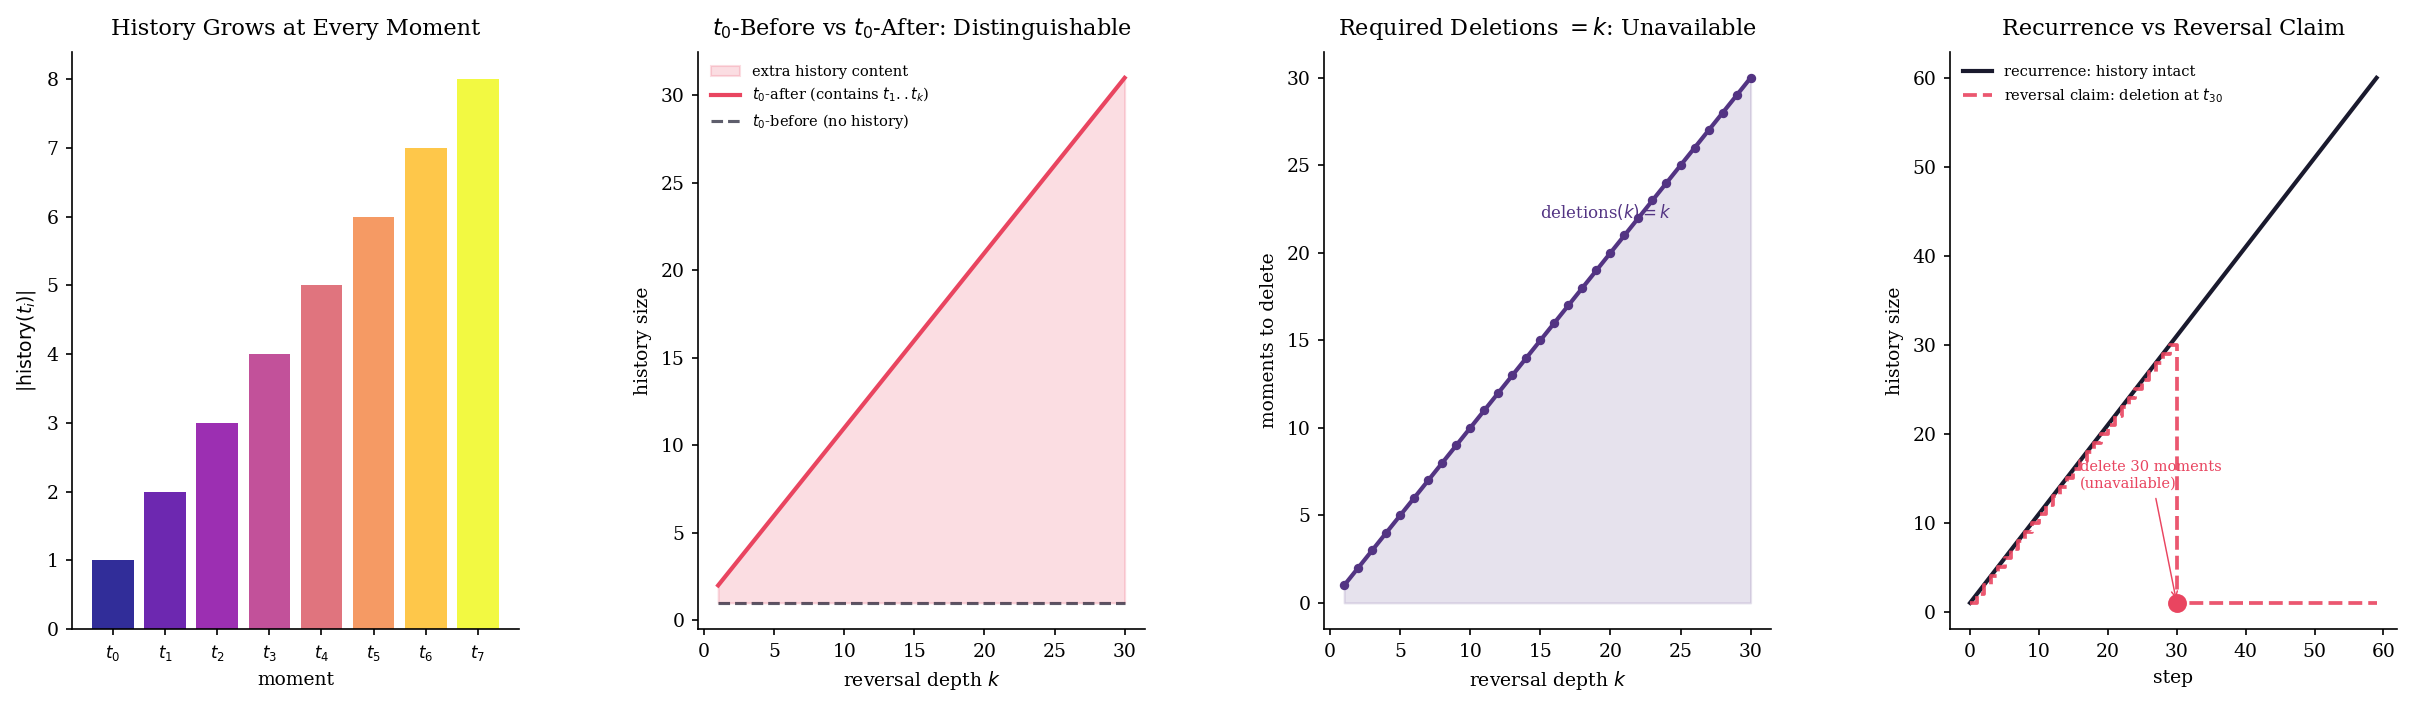
\includegraphics[width=\textwidth]{panels/panel_09_history_deletion.png}
    \caption{\textbf{Genuine time reversal from $t_k$ to $t_0$ requires deleting the
    intervening moments $t_1,\ldots,t_{k-1}$ from the universe's history; the required
    deletions grow linearly with reversal depth, and deletion is not an available
    physical operation
    (Theorems~\ref{thm:deletion} and~\ref{thm:no-deletion};
    Definition~\ref{def:distinguishability}).}
    (\textbf{A})~History size at each moment $t_i$: $|\mathrm{history}(t_i)| = i+1$,
    coloured by moment index (plasma scale).  History grows monotonically; no physical
    process reduces it.  The state at any moment includes the full causal record of all
    prior moments (Definition~\ref{def:distinguishability}).
    (\textbf{B})~State at $t_0$-before (history size $= 1$, dashed) versus state at
    $t_0$-after-reversal from depth $k$ (history size $= k+1$, solid), with shaded
    extra content.  The two states are distinguishable by their histories and are
    therefore distinct.  For the reversal claim to hold, the $k$ extra moments must be
    absent from the post-reversal state.
    (\textbf{C})~Required deletions as a function of reversal depth $k$:
    deletions$(k) = k$ exactly, growing linearly (shaded fill).  Any reversal of
    depth $k \geq 1$ requires at least one deletion; deletion is structurally
    unavailable (Theorem~\ref{thm:no-deletion}).
    (\textbf{D})~Recurrence (solid): history grows as the system evolves forward;
    at the recurrence step the configuration matches $t_0$ but the history is intact.
    Reversal claim (dashed): history would need to snap back to size $1$ at step $30$,
    requiring deletion of $30$ moments.  The sharp discontinuity marks the deletion
    event; no physical process produces it.  This panel directly visualises the
    distinction between recurrence and reversal established by
    Corollary~\ref{cor:egg-cycle}.}%
    \label{fig:panel9_history_deletion}
\end{figure*}

% ──────────────────────────────────────────────────────────────────────────────
\begin{figure*}[!htbp]
    \centering
    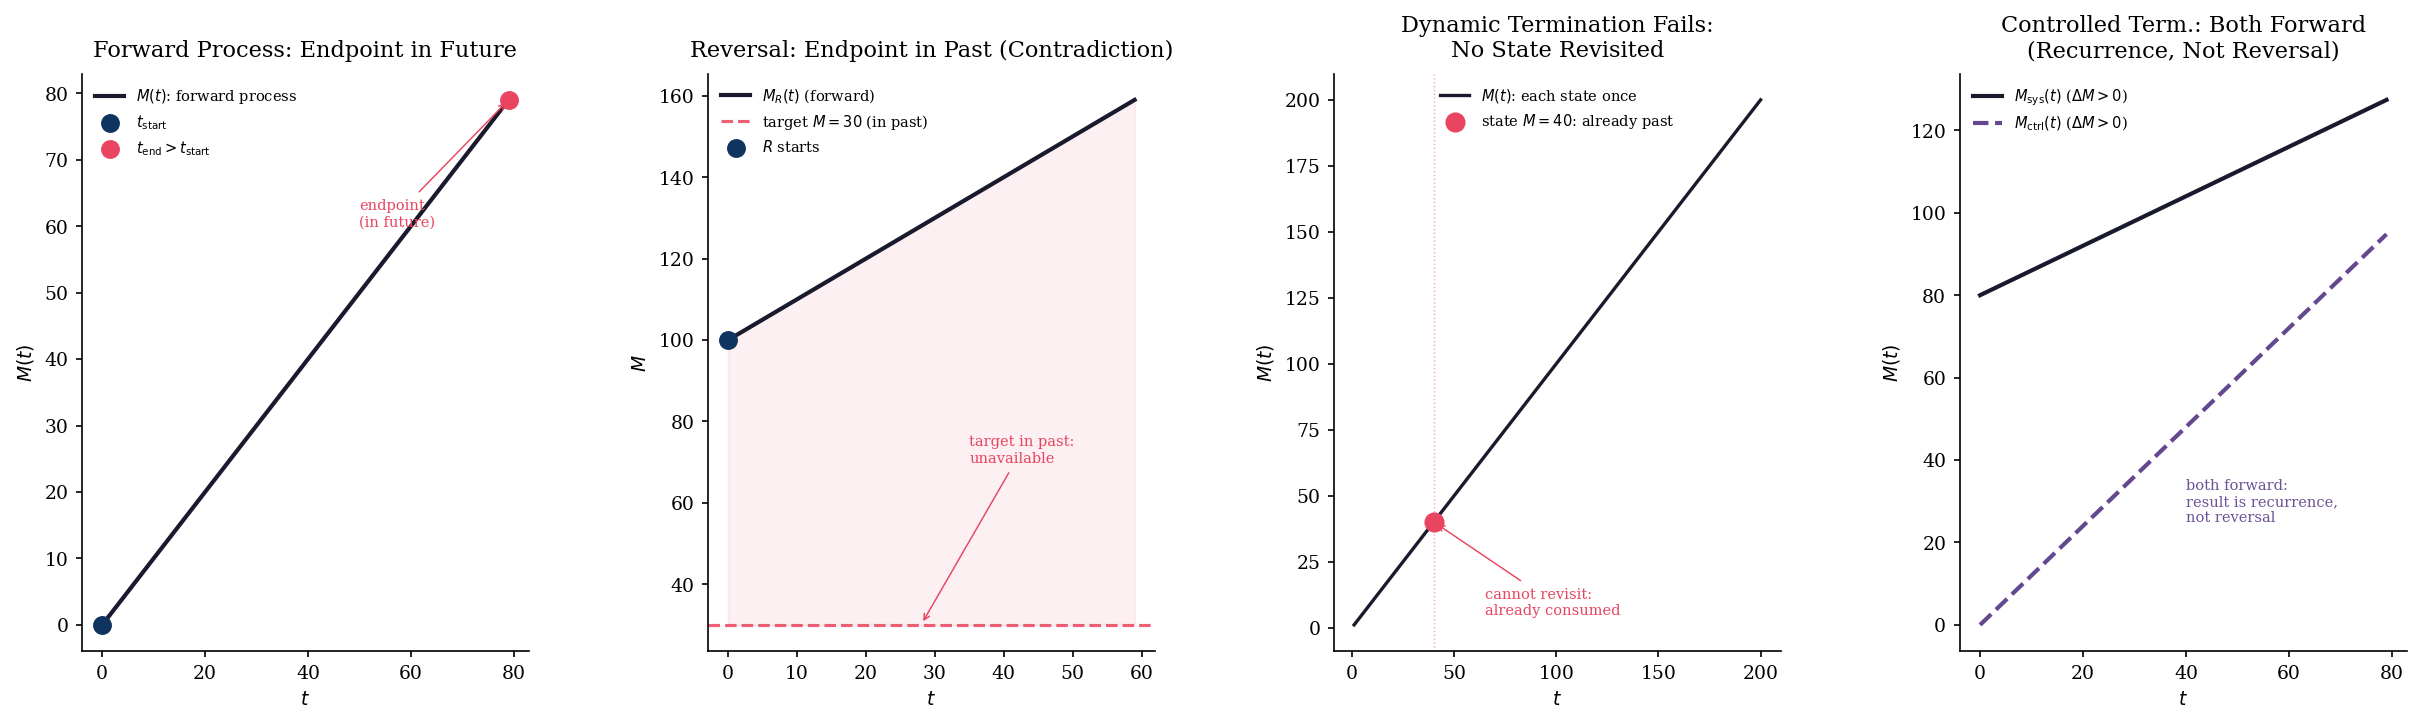
\includegraphics[width=\textwidth]{panels/panel_10_process_termination.png}
    \caption{\textbf{A reversal process $R$ has no available termination structure:
    its endpoint is a past state unreachable by dynamic termination
    (Corollary~\ref{cor:no-repeat}), and controlled termination collapses the reversal
    claim into a forward-time recurrence; no third mechanism exists
    (Theorem~\ref{thm:reversal-no-process}; Definition~\ref{def:process}).}
    (\textbf{A})~A forward process: $M(t)$ increases from $t_{\mathrm{start}}$ (blue) to
    $t_{\mathrm{end}}$ (orange).  The endpoint lies in the process's future; the
    forward dynamics determine when it is reached.  This is the canonical structure
    of any process in the sense of Definition~\ref{def:process}.
    (\textbf{B})~Putative reversal process $R$: $M_R(t)$ increases from $M = 100$ onward
    (forward time), but the target endpoint is the past state at $M = 30$ (dashed
    horizontal).  The gap between $M_R(t)$ and the target grows monotonically;
    dynamic termination cannot close this gap because the target recedes as $R$
    advances.
    (\textbf{C})~Dynamic termination fails: each partition state is visited exactly once
    along the forward trajectory (Corollary~\ref{cor:no-repeat}).  The state at
    $M = 40$ (orange marker) was consumed at step $40$ and cannot be revisited; a
    ``return'' requires a second visit, which the injectivity of $\Phi$ excludes.
    (\textbf{D})~Controlled termination yields recurrence, not reversal: both
    $M_{\mathrm{sys}}(t)$ (solid) and $M_{\mathrm{ctrl}}(t)$ (dashed) are strictly
    increasing.  The controller uses memory of a past configuration to navigate the
    system to a resembling configuration; both agents run forward.  This is a
    forward-time memory-driven recurrence of the kind formalised in
    Corollary~\ref{cor:egg-cycle}, not genuine reversal.}%
    \label{fig:panel10_process_termination}
\end{figure*}

% after the figures are placed in the manuscript.

% ──────────────────────────────────────────────────────────────────────────────
\begin{figure*}[!htbp]
    \centering
    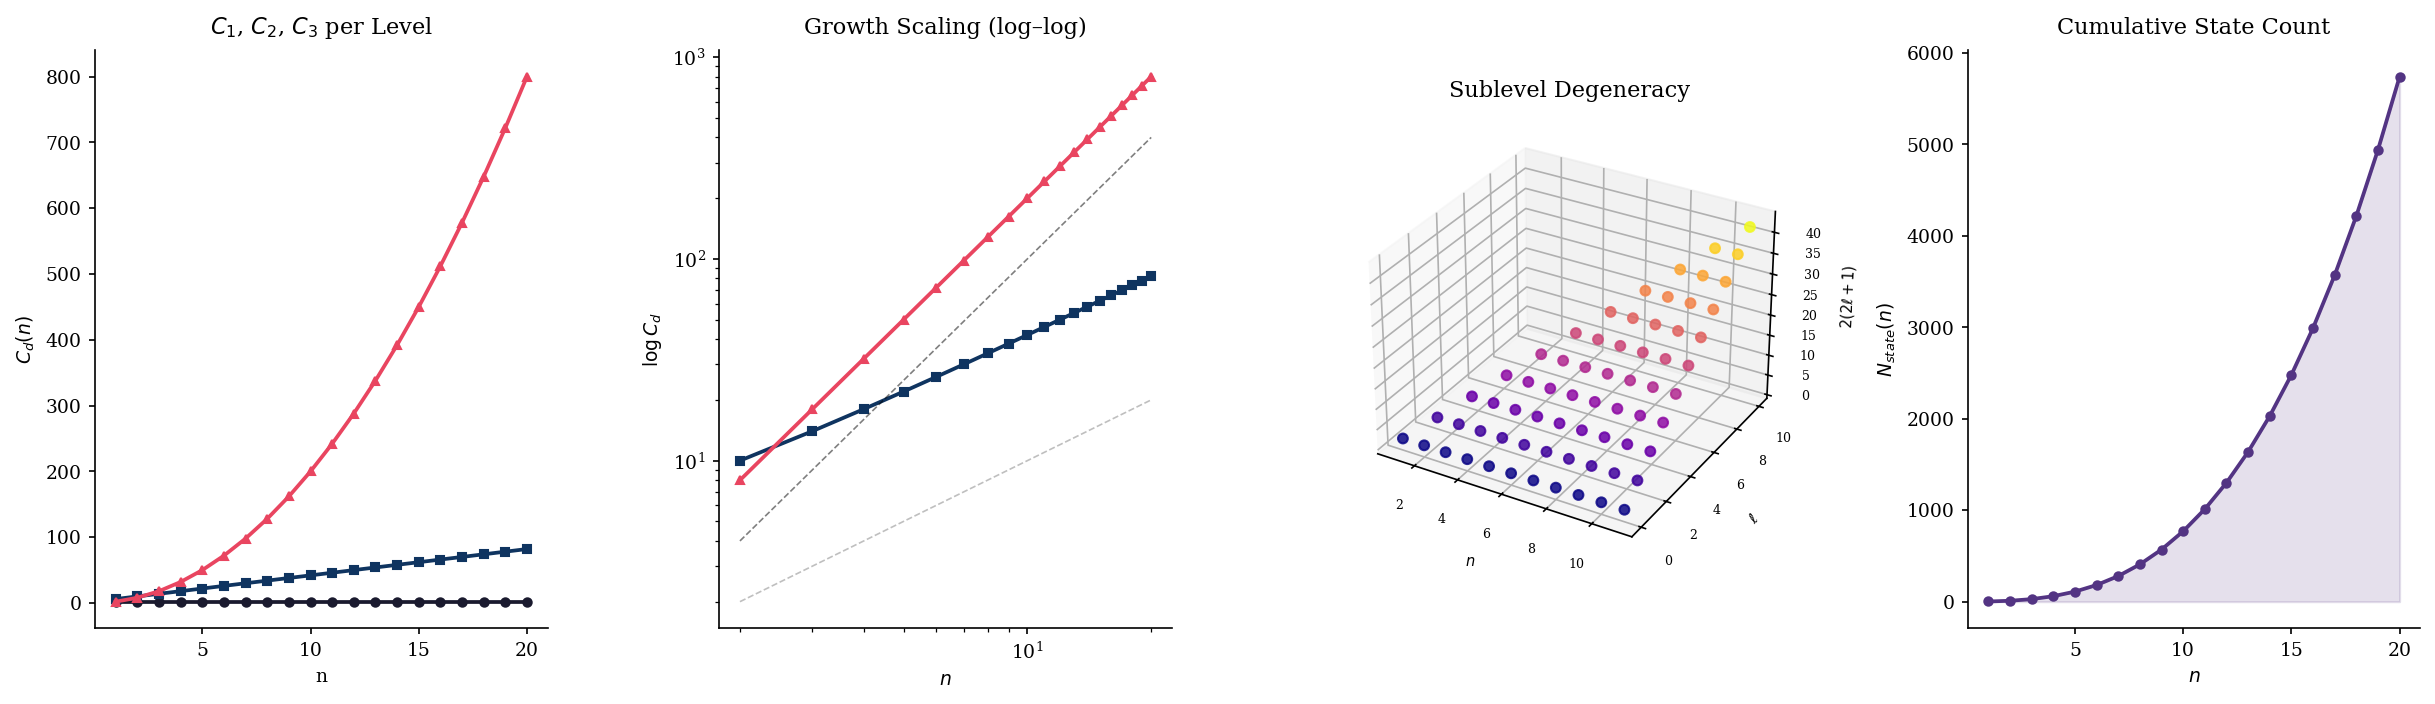
\includegraphics[width=\textwidth]{panels/panel_01_capacity_hierarchy.png}
    \caption{\textbf{Capacity growth $C_d(n)$ is constant in $d{=}1$, linear in $d{=}2$, and
    quadratic in $d{=}3$, establishing a strict dimensional hierarchy whose slope on a
    log–log axis discriminates the angular dimension of each within-level partition space
    (Definition~\ref{def:cap-d}; Theorem~\ref{thm:capacity}).}
    (\textbf{A})~Line plot of per-level capacity $C_d(n)$ versus principal quantum number $n$
    for $d{=}1$ (dark, flat), $d{=}2$ (mid, linear), and $d{=}3$ (light, quadratic).
    The three curves separate immediately at $n{=}2$: $C_1$ remains fixed at $2$; $C_2$
    grows as $4n{+}2$; $C_3 = 2n^2$ accelerates away from both, reflecting the
    two-dimensional angular structure of the within-level space $L_n^{(3)}$.
    (\textbf{B})~Log–log plot of $C_2(n)$ and $C_3(n)$ for $n \geq 3$, overlaid with reference
    lines of slope $1$ (linear, grey dashed) and slope $2$ (quadratic, black dashed).
    $C_2$ tracks the slope-$1$ reference exactly; $C_3$ tracks slope $2$ exactly,
    confirming that the exponent of capacity growth equals the continuous angular
    dimension of $L_n^{(d)}$: $0$ for $d{=}1$, $1$ for $d{=}2$, $2$ for $d{=}3$.
    (\textbf{C})~Three-dimensional scatter of sublevel degeneracy $2(2\ell+1)$ plotted against
    principal level $n$ (x-axis) and angular index $\ell$ (y-axis) for $n = 1,\ldots,11$.
    Colour encodes degeneracy magnitude (plasma scale).  The surface rises along both
    axes, with the steepest growth in $\ell$ at fixed $n$, reproducing the quadratic
    capacity as $C_3(n) = \sum_{\ell=0}^{n-1} 2(2\ell{+}1)$.
    (\textbf{D})~Line plot of cumulative state count $N_\mathrm{state}(n) = n(n{+}1)(2n{+}1)/3$
    versus $n$ with shaded fill.  The cubic growth follows directly from summing the
    quadratic per-level capacity; the steepening curvature is the algebraic signature
    that each added level contributes an accelerating number of partition states, as
    stated in Corollary~\ref{cor:cumulative}.}%
    \label{fig:panel1_capacity_hierarchy}
\end{figure*}

% ──────────────────────────────────────────────────────────────────────────────
\begin{figure*}[!htbp]
    \centering
    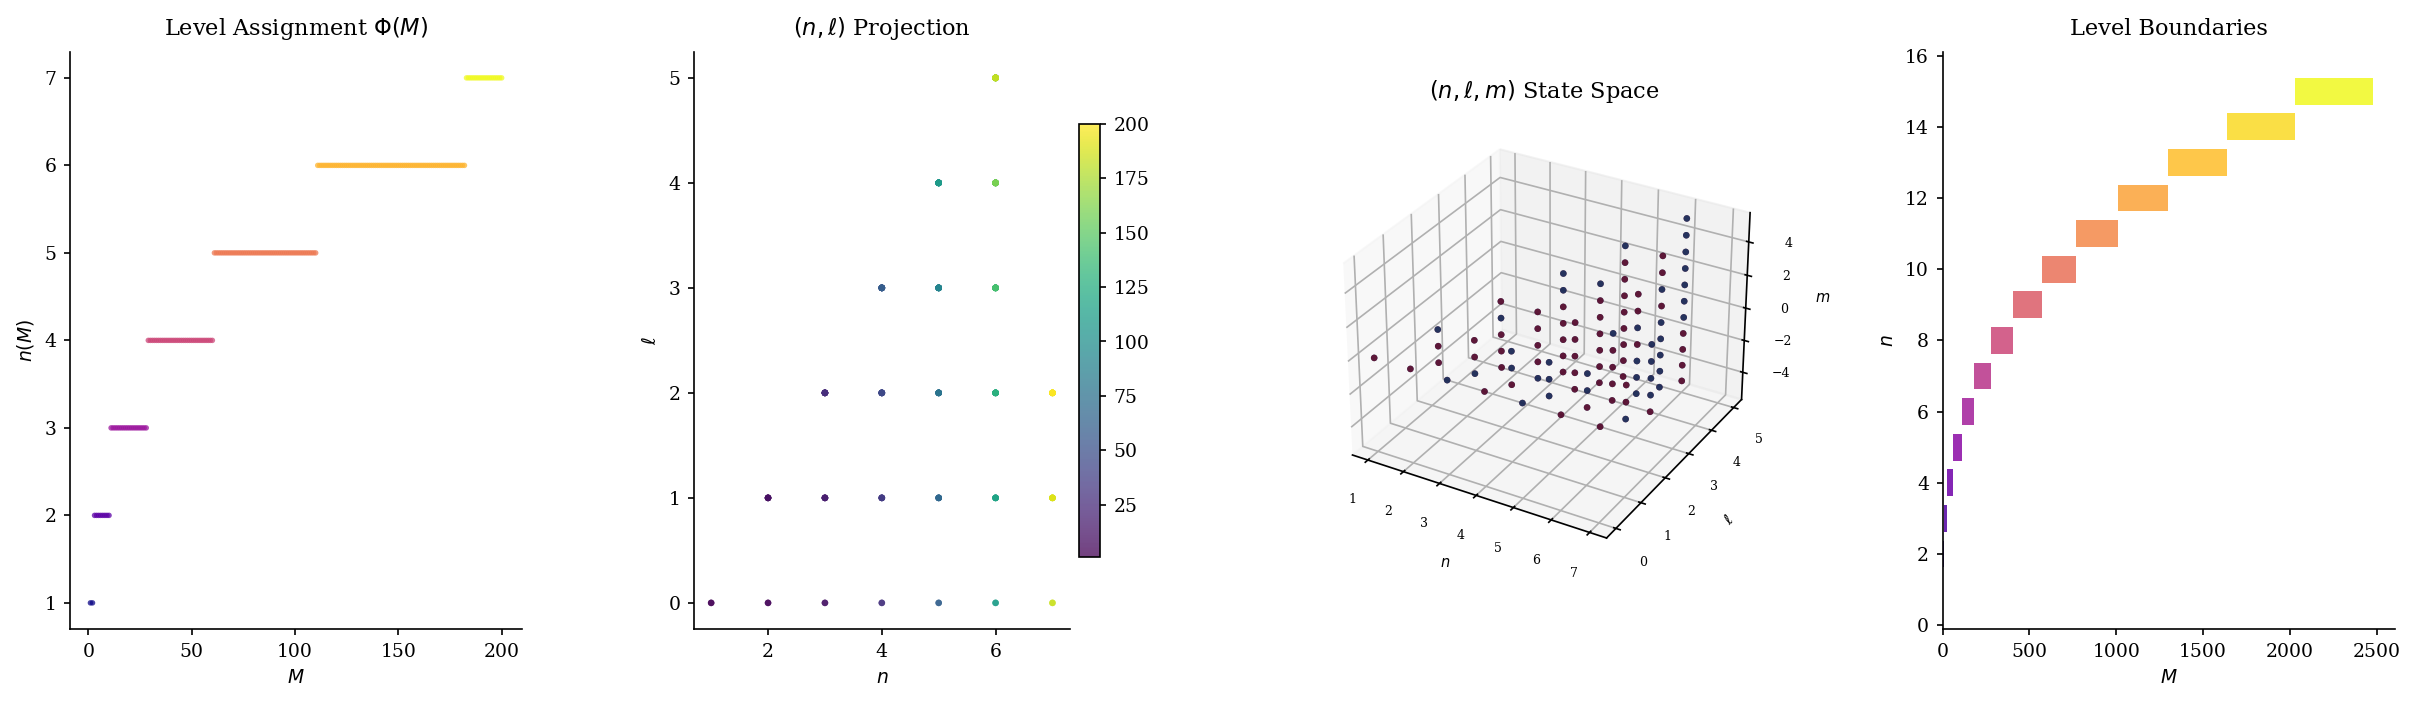
\includegraphics[width=\textwidth]{panels/panel_02_bijection_structure.png}
    \caption{\textbf{The partition map $\Phi:\mathbb{Z}^{+}\!\to\mathcal{P}$ is a
    well-defined bijection whose image tiles three-dimensional quantum-number space
    without collision or gap, and whose level boundaries are sharp staircase
    transitions determined by the cumulative capacity formula
    (Theorem~\ref{thm:bijection}; Corollary~\ref{cor:cumulative}).}
    (\textbf{A})~Scatter of principal level $n(\Phi(M))$ versus integer index $M$ for
    $M = 1,\ldots,200$, coloured by $n$ (plasma scale).  Level transitions appear as
    discrete upward steps; within each band $M$ increments uniformly, confirming
    that $\Phi$ exhausts every state of level $n$ before advancing to $n{+}1$.
    (\textbf{B})~Two-dimensional projection onto the $(n,\ell)$ plane, coloured by $M$
    (viridis scale).  Each point $(n,\ell)$ appears with multiplicity $2(2\ell{+}1)$,
    one for each $(m,s)$ pair; the colour gradient shows that $M$ increases
    monotonically left-to-right and bottom-to-top within each level, establishing
    the lexicographic ordering of $\Phi$.
    (\textbf{C})~Three-dimensional scatter of the full quantum-number triple $(n,\ell,m)$
    for $M = 1,\ldots,200$, with colour encoding spin $s = \pm\tfrac{1}{2}$ (red–blue
    diverging scale).  The cloud fills a triangular prism in $(n,\ell,m)$ space:
    $0 \leq \ell \leq n{-}1$, $-\ell \leq m \leq \ell$.  No two points coincide,
    providing visual confirmation of injectivity (Theorem~\ref{thm:bijection}).
    (\textbf{D})~Horizontal bar chart of level sizes: each bar spans the $M$-range
    $[N_\mathrm{state}(n{-}1){+}1,\, N_\mathrm{state}(n)]$ for levels $n = 1,\ldots,15$,
    coloured by level index.  Bar widths equal $C_3(n) = 2n^2$, growing quadratically;
    the staircase of left boundaries locates the exact $M$-index at which each new
    principal level begins, as derived in Corollary~\ref{cor:cumulative}.}%
    \label{fig:panel2_bijection_structure}
\end{figure*}

% ──────────────────────────────────────────────────────────────────────────────
\begin{figure*}[!htbp]
    \centering
    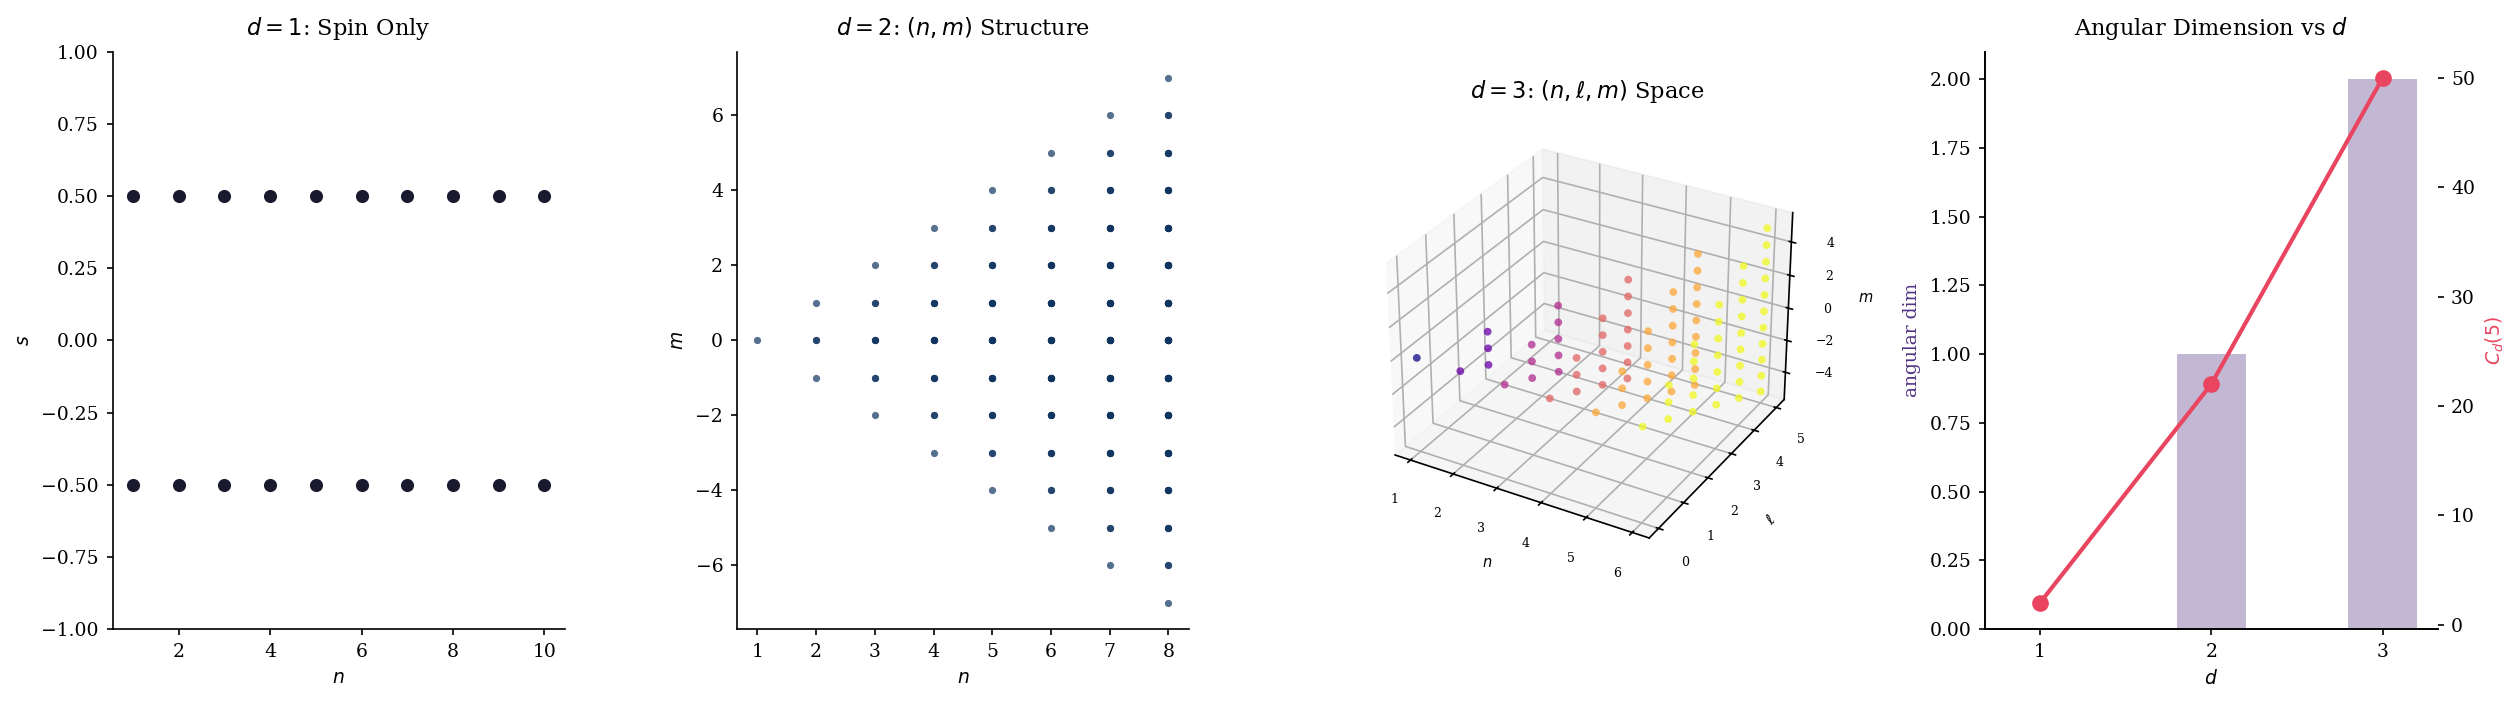
\includegraphics[width=\textwidth]{panels/panel_03_partition_geometry.png}
    \caption{\textbf{Spatial dimension $d{=}3$ is the minimum for which the within-level
    partition space $L_n^{(d)}$ has continuous angular dimension $\geq 2$, enabling
    negation to close around any state from all angular directions simultaneously
    (Theorem~\ref{thm:min-dim}; Definition~\ref{def:within-level}).}
    (\textbf{A})~Scatter of partition states in $d{=}1$: only the spin coordinate $s =
    \pm\tfrac{1}{2}$ varies; every level $n$ contributes exactly two isolated points.
    The within-level space $L_n^{(1)}$ has angular dimension $0$: there is no
    continuous angular degree of freedom, so negation from the ``left'' and ``right''
    cannot simultaneously enclose the state.
    (\textbf{B})~Scatter of partition states $(n, m)$ for $d{=}2$, $n = 1,\ldots,8$.
    Within level $n$, the $m$-values $\{-(n{-}1),\ldots,n{-}1\}$ form a one-dimensional
    chain; $L_n^{(2)}$ has angular dimension $1$.  Two opposing states can bracket any
    given $m$, but the within-level topology is a line segment, not a closed surface,
    so negation-closure is incomplete.
    (\textbf{C})~Three-dimensional scatter of partition states $(n, \ell, m)$ for $d{=}3$,
    $n = 1,\ldots,6$, coloured by $n$ (plasma scale).  Within level $n$, the pairs
    $(\ell, m)$ fill a two-dimensional triangular region; $L_n^{(3)}$ has angular
    dimension $2$.  Every interior point is enclosed from all angular directions,
    satisfying the closure condition of Theorem~\ref{thm:min-dim}.
    (\textbf{D})~Combined bar and line chart comparing angular dimension (left axis, bars)
    and per-level capacity $C_d(5)$ (right axis, line with markers) for $d = 1, 2, 3$.
    Angular dimension steps $0 \to 1 \to 2$ in exact correspondence with the
    exponent governing $C_d$, confirming that the quadratic capacity of $d{=}3$ is the
    algebraic signature of the minimum dimensionality required for
    negation-constituted closure.}%
    \label{fig:panel3_partition_geometry}
\end{figure*}

% ──────────────────────────────────────────────────────────────────────────────
\begin{figure*}[!htbp]
    \centering
    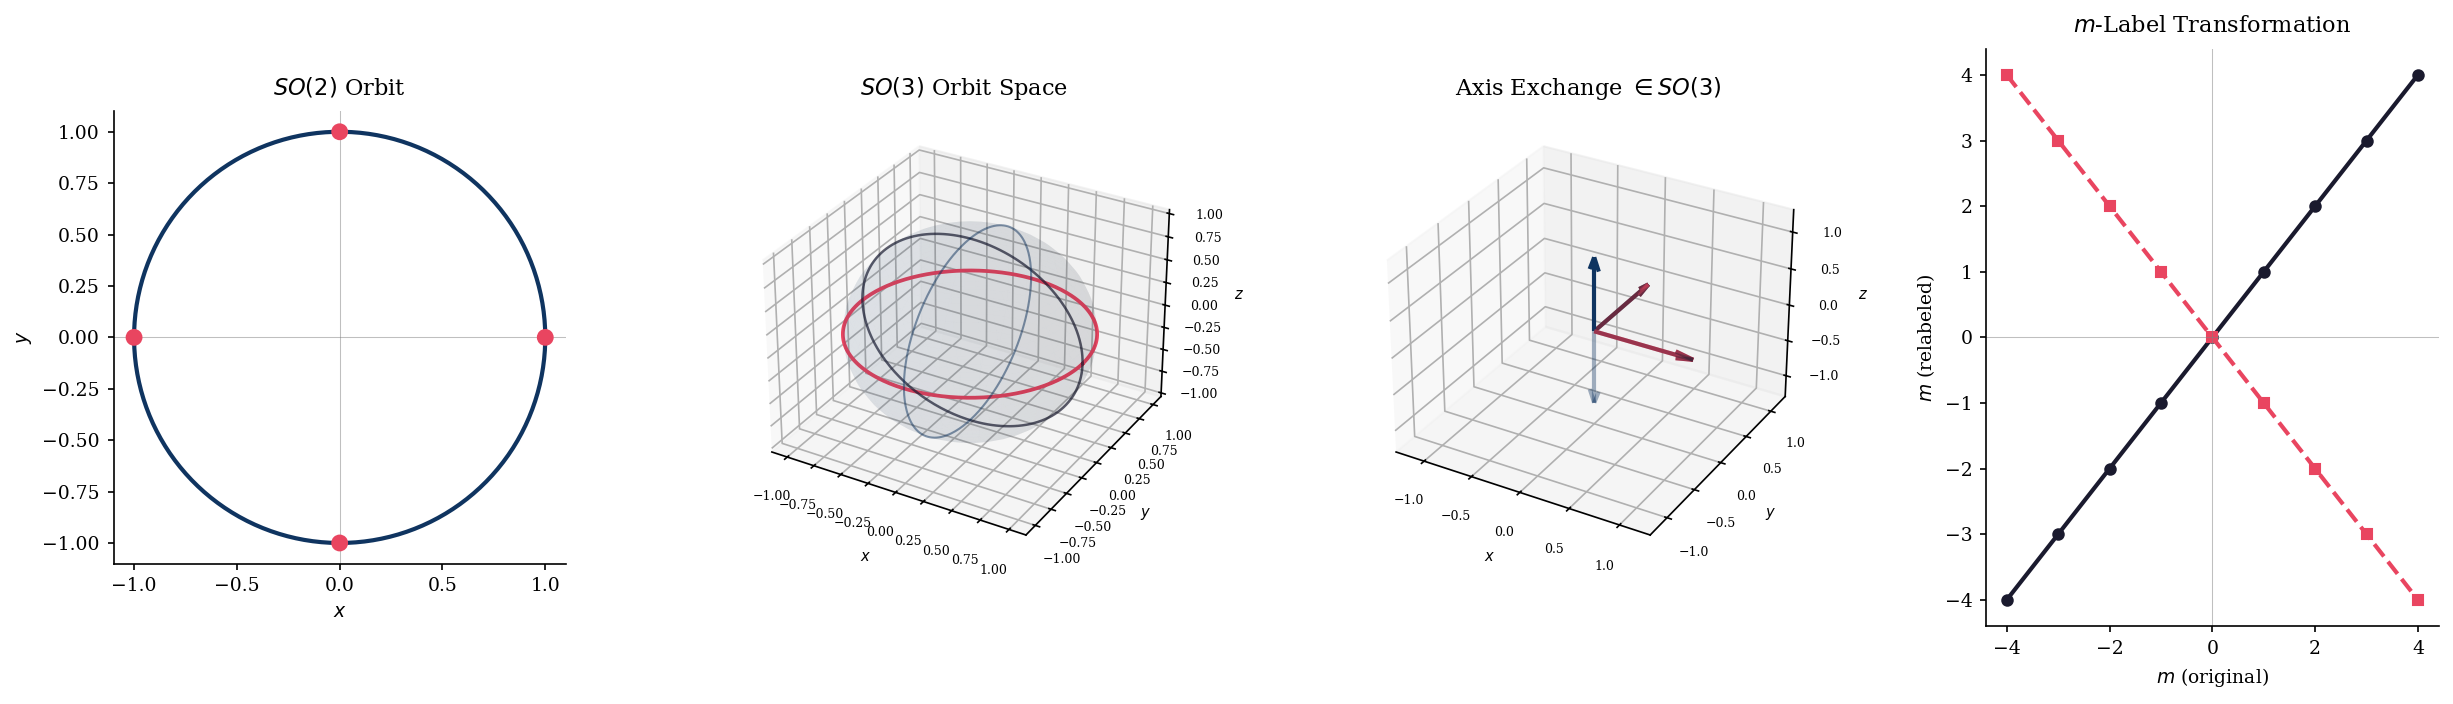
\includegraphics[width=\textwidth]{panels/panel_04_SO3_symmetry.png}
    \caption{\textbf{The axis exchange $(x,y,z)\mapsto(y,x,-z)$ is a proper rotation
    in $SO(3)$ with $\det = +1$, but the analogous swap $x \leftrightarrow y$ in
    $d{=}2$ is an improper reflection with $\det = -1$; consequently, the
    $m$-label is $SO(2)$-invariant but changes under $SO(3)$ axis relabelling,
    and partition identity is reference-frame-independent only for $d\geq 3$
    (Corollary~\ref{cor:axis-exchange}).}
    (\textbf{A})~$SO(2)$ orbit: unit circle in the $xy$-plane with four marked points at
    $(\pm 1, 0)$ and $(0, \pm 1)$.  All rotations in $SO(2)$ preserve orientation;
    the swap $x \leftrightarrow y$ in two dimensions corresponds to reflection
    across the diagonal, an element of $O(2) \setminus SO(2)$ with $\det = -1$.
    (\textbf{B})~$SO(3)$ orbit space: transparent unit sphere with equatorial orbit
    (coloured ring, equator plane) and two meridional great-circle orbits.  The full
    $SO(3)$ orbit of a fixed axis direction sweeps a two-sphere, capturing the
    additional degree of freedom absent in $d{=}2$.
    (\textbf{C})~Three-dimensional axis-frame diagram visualising the exchange
    $R: (x,y,z)\mapsto(y,x,-z)$.  Solid arrows show the original frame
    $(\hat{e}_x, \hat{e}_y, \hat{e}_z)$; translucent arrows show the relabelled
    frame.  This transformation lies in $SO(3)$ ($\det R = +1$, angle $=\pi$ about
    the axis $\frac{1}{\sqrt{2}}(\hat{e}_x + \hat{e}_y)$), making it a physically
    accessible change of reference frame rather than an orientation reversal.
    (\textbf{D})~Line plot of the $m$-label transformation for $\ell = 4$ under the two
    symmetry groups.  Under $SO(2)$ rotation about $\hat{z}$, the eigenvalue $m$
    is invariant (identity line, dark).  Under the $SO(3)$ axis exchange of panel
    (C), $L_z \to -L_z$ and $m \mapsto -m$ (reflected line, light).  The
    non-trivial relabelling confirms that $m$ encodes a reference-frame choice,
    not an observer-independent integer, whenever $d \geq 3$.}%
    \label{fig:panel4_SO3_symmetry}
\end{figure*}

% ──────────────────────────────────────────────────────────────────────────────
\begin{figure*}[!htbp]
    \centering
    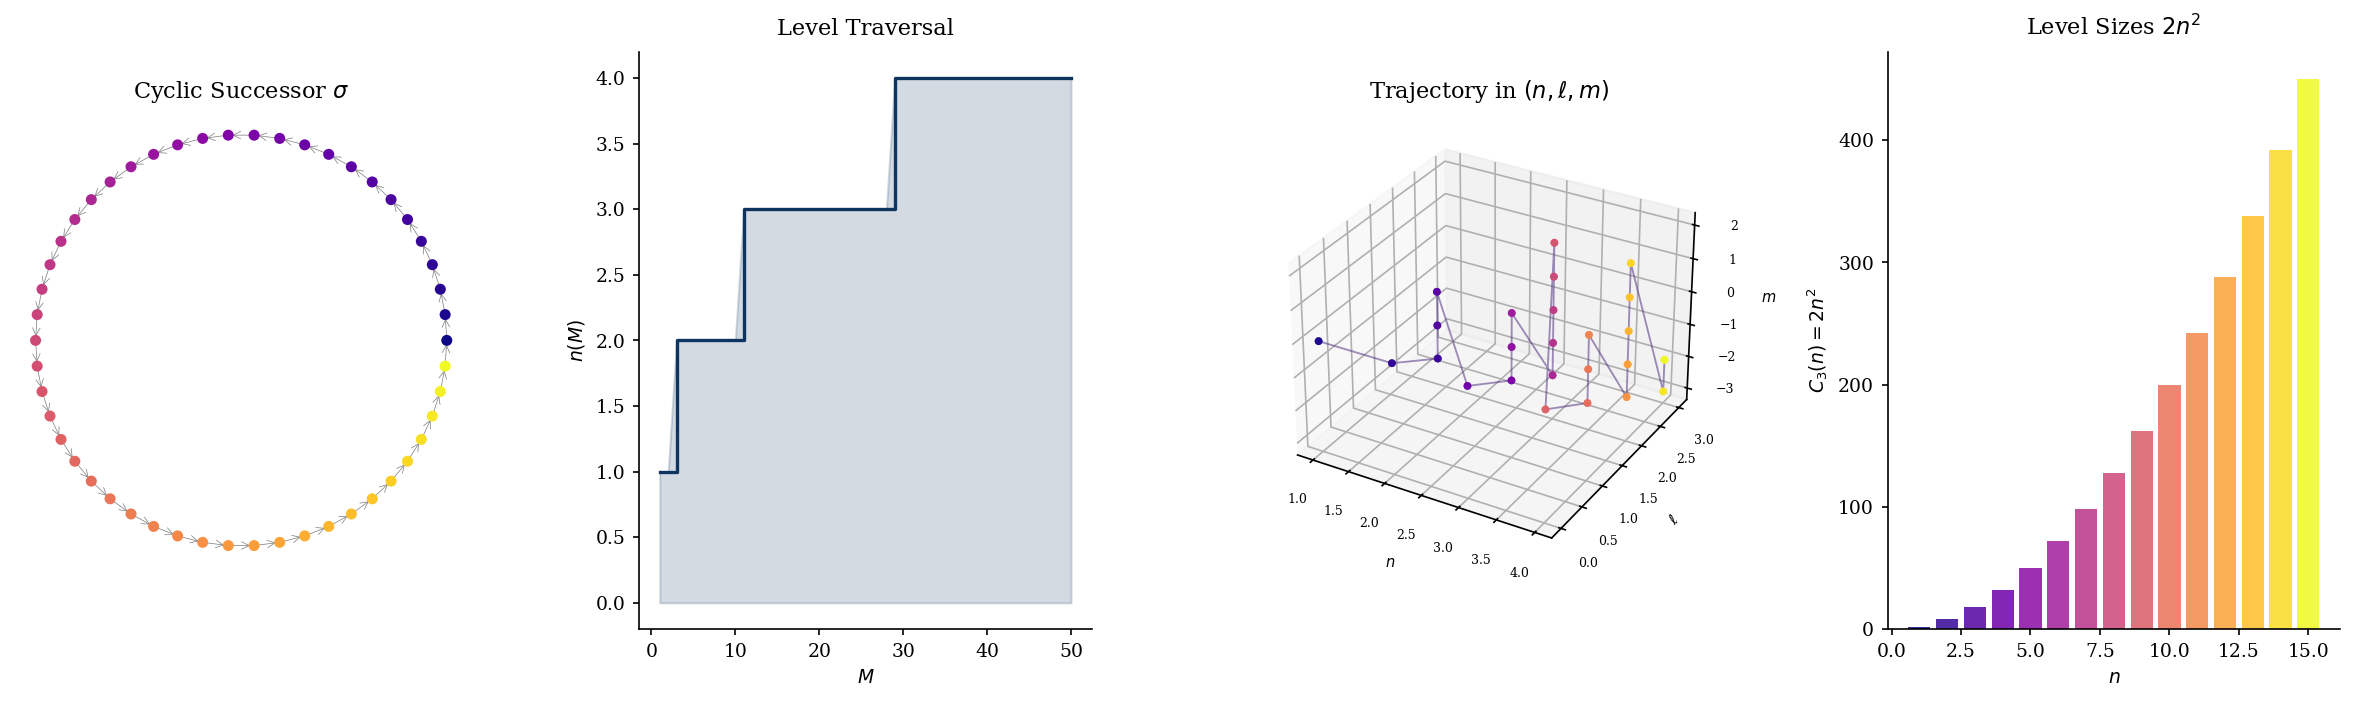
\includegraphics[width=\textwidth]{panels/panel_05_cyclic_closure.png}
    \caption{\textbf{The successor relation $\sigma$ is a bijection on the finite partition
    category $\mathcal{C}$ whose unique cycle has length $M_{\max} = N_\mathrm{state}(n_{\max})$,
    forcing every state—including $\Phi(1)$—to be revisited exactly once per period and
    making cyclic closure a structural consequence of finiteness rather than a dynamical
    assumption (Theorem~\ref{thm:cyclic}; Theorem~\ref{thm:cat-closure}).}
    (\textbf{A})~Cyclic successor diagram for $M_{\max} = 50$: each partition state is
    placed on a unit circle at angle $2\pi M / M_{\max}$, coloured by $M$ (plasma
    scale), with grey arrows connecting $\Phi(M)$ to $\sigma(\Phi(M)) = \Phi(M{+}1)$.
    The final arrow from $\Phi(50)$ returns to $\Phi(1)$, completing the cycle and
    confirming that $\sigma$ is a permutation of $\mathcal{C}$ with no fixed points
    and no proper sub-cycles (Theorem~\ref{thm:cyclic}).
    (\textbf{B})~Step plot of the level assignment $n(M)$ for $M = 1,\ldots,50$, with
    shaded fill below the curve.  Each plateau spans exactly $C_3(n) = 2n^2$ consecutive
    integers; the risers are instantaneous, reflecting the sharp level boundary at
    $M = N_\mathrm{state}(n)$.  The sequence is strictly non-decreasing (Theorem~\ref{thm:monotone}),
    encoding the irreversibility of temporal progression within the bijective ordering.
    (\textbf{C})~Three-dimensional trajectory through $(n, \ell, m)$ state space for
    $M = 1,\ldots,50$, with points coloured by $M$ (plasma scale) and connected by a
    curve.  The path climbs through successive levels, executes a zig-zag pattern
    within each level as $\ell$ and $m$ increment lexicographically, then returns to
    the origin upon cyclic closure.  The trajectory is injective on any open arc but
    closed as a whole (Corollary~\ref{cor:cyclic}).
    (\textbf{D})~Bar chart of level sizes $C_3(n) = 2n^2$ for $n = 1,\ldots,15$, coloured
    by level index.  Quadratic growth of bar height reflects the quadratic capacity law;
    the total area equals $M_{\max} = N_\mathrm{state}(n_{\max})$, the unique cycle length.
    The accelerating size of successive levels means that higher-$n$ states are
    structurally ``harder to reach'' in the sense of requiring a longer prefix of
    the successor sequence.}%
    \label{fig:panel5_cyclic_closure}
\end{figure*}

% ──────────────────────────────────────────────────────────────────────────────
\begin{figure*}[!htbp]
    \centering
    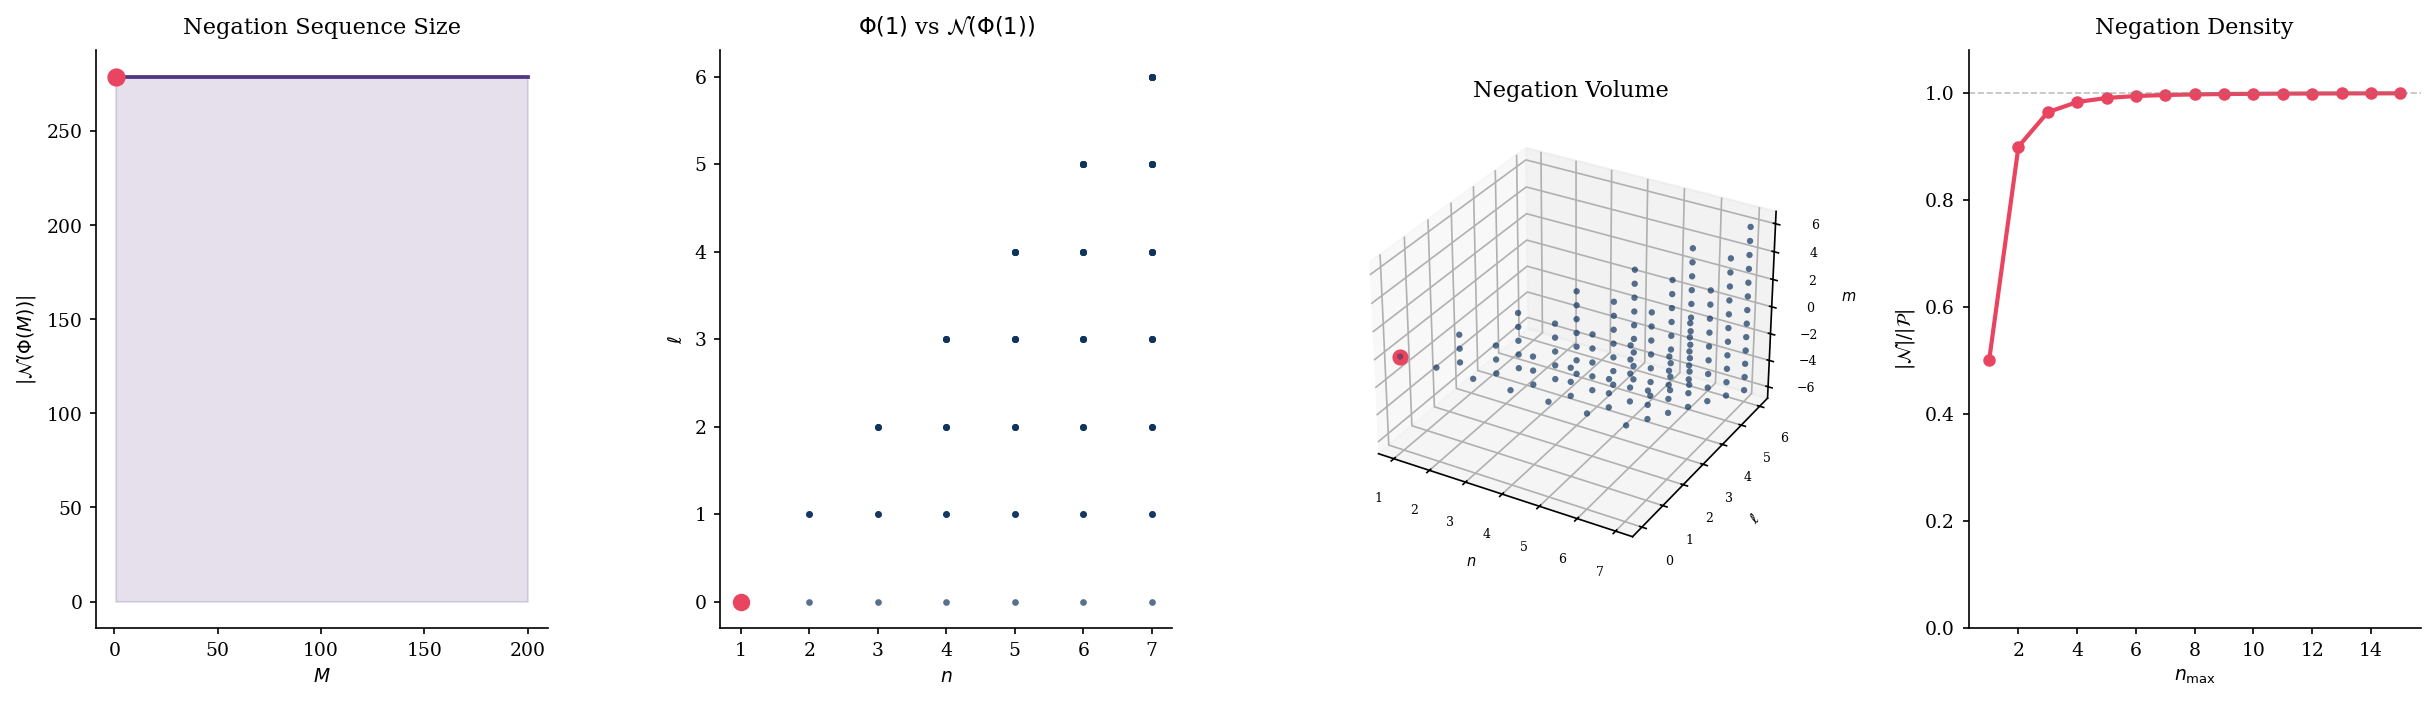
\includegraphics[width=\textwidth]{panels/panel_06_negation_identity.png}
    \caption{\textbf{Every partition state $\Phi(M)$ is uniquely identified by its negation
    sequence $\mathcal{N}(\Phi(M)) = \mathcal{P} \setminus \{\Phi(M)\}$, and the ground
    state $\Phi(1) = (1,0,0,+\tfrac{1}{2})$ possesses the largest possible negation
    sequence while being categorically irreducible, making it the structurally necessary
    origin of the partition sequence
    (Theorem~\ref{thm:negation-duality}; Definition~\ref{def:ground-cat};
    Theorem~\ref{thm:sing-necessity}).}
    (\textbf{A})~Scatter and fill of $|\mathcal{N}(\Phi(M))| = |\mathcal{P}| - 1$ versus $M$
    for $M = 1,\ldots,200$.  The value is constant across all $M$: every state has
    exactly one fewer element in its negation sequence than the cardinality of
    $\mathcal{P}$, because negation excludes only $\Phi(M)$ itself.  The ground state
    $\Phi(1)$ is marked (orange dot); it is distinguished not by a different negation
    size but by the property that $\Phi(1)$ has no $\sigma$-predecessor in
    $\mathcal{P}$ (Theorem~\ref{thm:sing-necessity}).
    (\textbf{B})~Two-dimensional scatter of the full partition space projected onto
    $(n, \ell)$ for $n = 1,\ldots,7$.  All states except $\Phi(1) = (1,0,0,+\tfrac{1}{2})$
    are shown in blue (the negation sequence $\mathcal{N}(\Phi(1))$); $\Phi(1)$ is marked
    in orange.  The visual contrast makes precise the duality $\mathcal{P} =
    \{\Phi(1)\} \cup \mathcal{N}(\Phi(1))$: identity is constituted by the totality
    of what it is not (Theorem~\ref{thm:negation-duality}).
    (\textbf{C})~Three-dimensional scatter of the full partition space in $(n, \ell, m)$
    for $n = 1,\ldots,7$.  Blue points form the negation volume $\mathcal{N}(\Phi(1))$;
    the single orange point at the origin $(1,0,0)$ is the ground state $\Phi(1)$.
    The geometric relationship captures the categorical claim: $\Phi(1)$ is the unique
    state maximally enclosed by its own negation set from all angular directions in
    the three-dimensional partition space.
    (\textbf{D})~Line plot of the negation density ratio $|\mathcal{N}| / |\mathcal{P}_{n_{\max}}|$
    versus the truncation level $n_{\max}$, where $|\mathcal{P}_{n_{\max}}| =
    N_\mathrm{state}(n_{\max})$.  The ratio $(N - 1)/N$ increases monotonically toward $1$
    as $n_{\max} \to \infty$, with the horizontal dashed line marking the asymptotic
    limit.  This convergence is the quantitative expression of the remark that any
    finite physical category saturates the negation relation: as the category grows,
    a state's identity becomes more fully determined by what it is not, with the
    ground state $\Phi(1)$ retaining the maximum negation complement at every
    finite truncation.}%
    \label{fig:panel6_negation_identity}
\end{figure*}

% ──────────────────────────────────────────────────────────────────────────────
\begin{figure*}[!htbp]
    \centering
    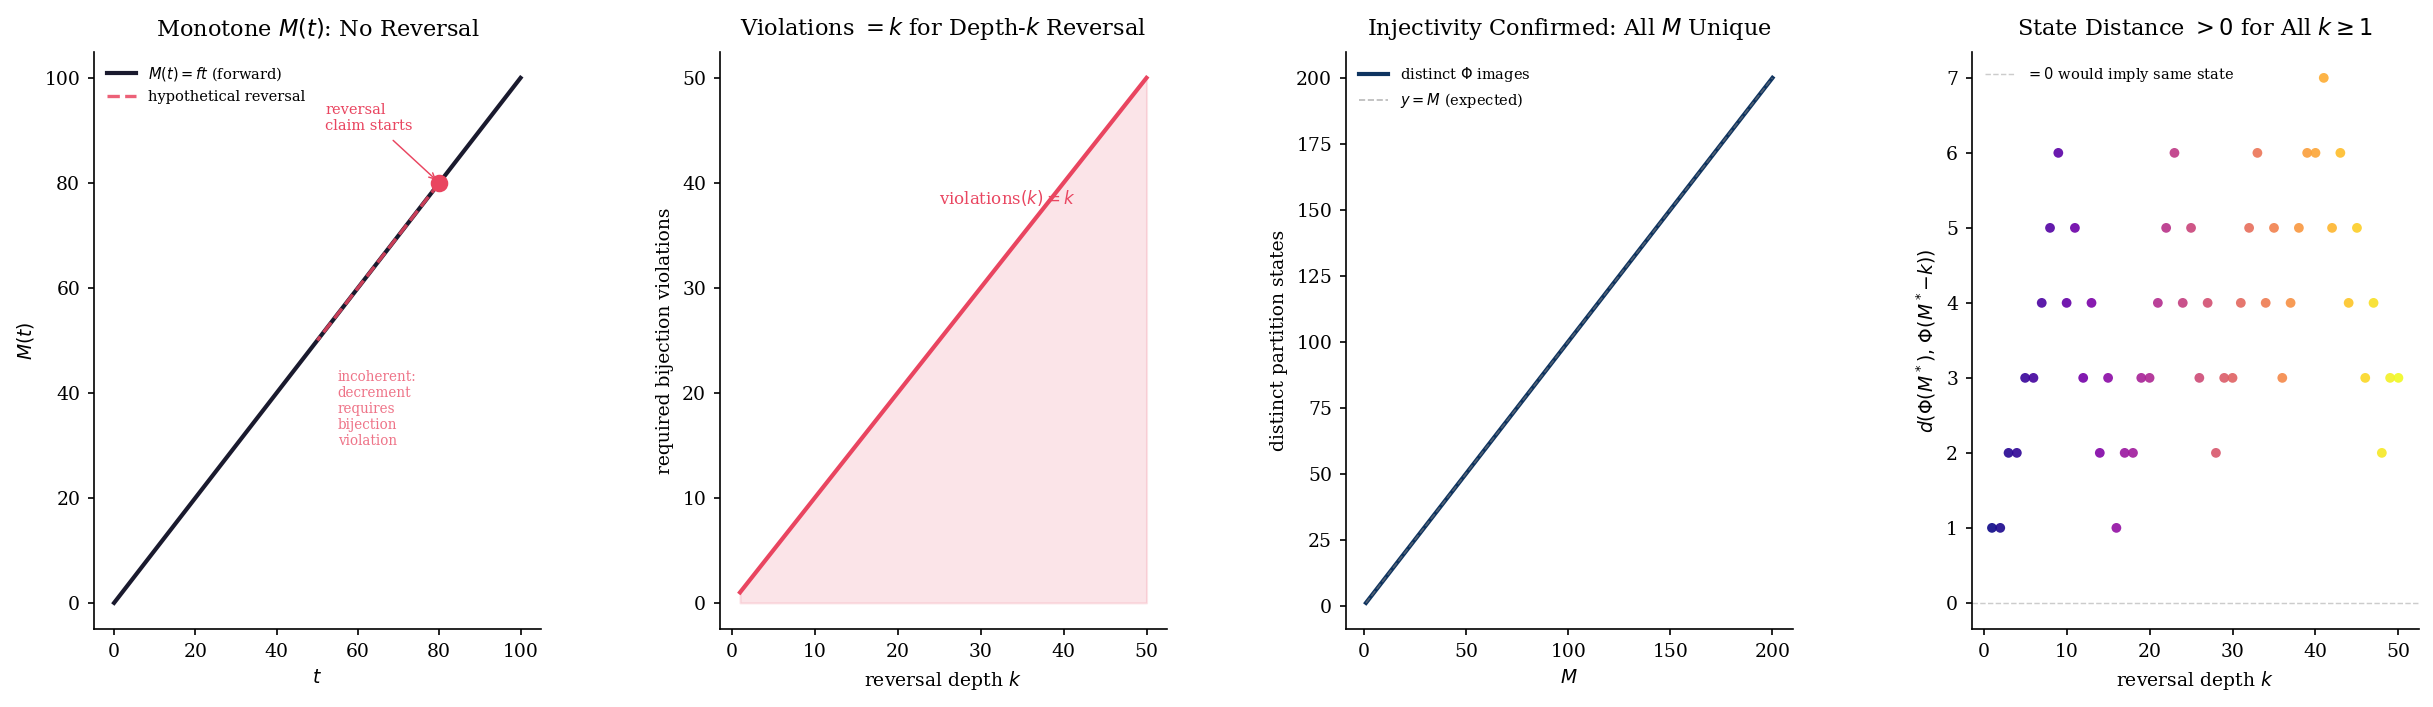
\includegraphics[width=\textwidth]{panels/panel_07_decrement_incoherence.png}
    \caption{\textbf{Any decrement $M \to M{-}k$ requires the bijection $\Phi$ to assign
    the same partition state to two distinct positive integers, violating injectivity;
    the number of required violations grows linearly with reversal depth $k$
    (Theorem~\ref{thm:incoherence}; Corollary~\ref{cor:loschmidt}).}
    (\textbf{A})~The partition count $M(t) = ft$ is strictly monotone (solid).  A
    hypothetical reversal segment (dashed, originating at $M = 80$) is shown; this
    trajectory has no physical realisation because no operation on the counting process
    corresponds to $\Delta M < 0$.
    (\textbf{B})~Required bijection violations as a function of reversal depth $k$,
    for a reversal originating at $M^{*} = 100$: violations$(k) = k$ exactly.  A
    depth-$k$ reversal forces $k$ distinct integers in $\Zp$ to share a single image
    under $\Phi$, contradicting Theorem~\ref{thm:bijection}.
    (\textbf{C})~Running count of distinct $\Phi$-images for $M = 1,\ldots,200$ (solid)
    overlaid on the identity line $y = M$ (dashed).  The two coincide exactly,
    confirming that all $200$ partition states are distinct and the bijection is
    injective with no collisions: the formal argument's central claim verified
    numerically at $M = 200$.
    (\textbf{D})~Manhattan distance $d(\Phi(M^{*}),\,\Phi(M^{*}{-}k))$ in partition-label
    space for $M^{*} = 100$, $k = 1,\ldots,50$, coloured by $k$ (plasma scale).
    Every distance is strictly positive: no two distinct integers share a
    partition-state image, confirming that any claimed decrement produces a genuine
    collision, not a near-miss.}%
    \label{fig:panel7_decrement_incoherence}
\end{figure*}

% ──────────────────────────────────────────────────────────────────────────────
\begin{figure*}[!htbp]
    \centering
    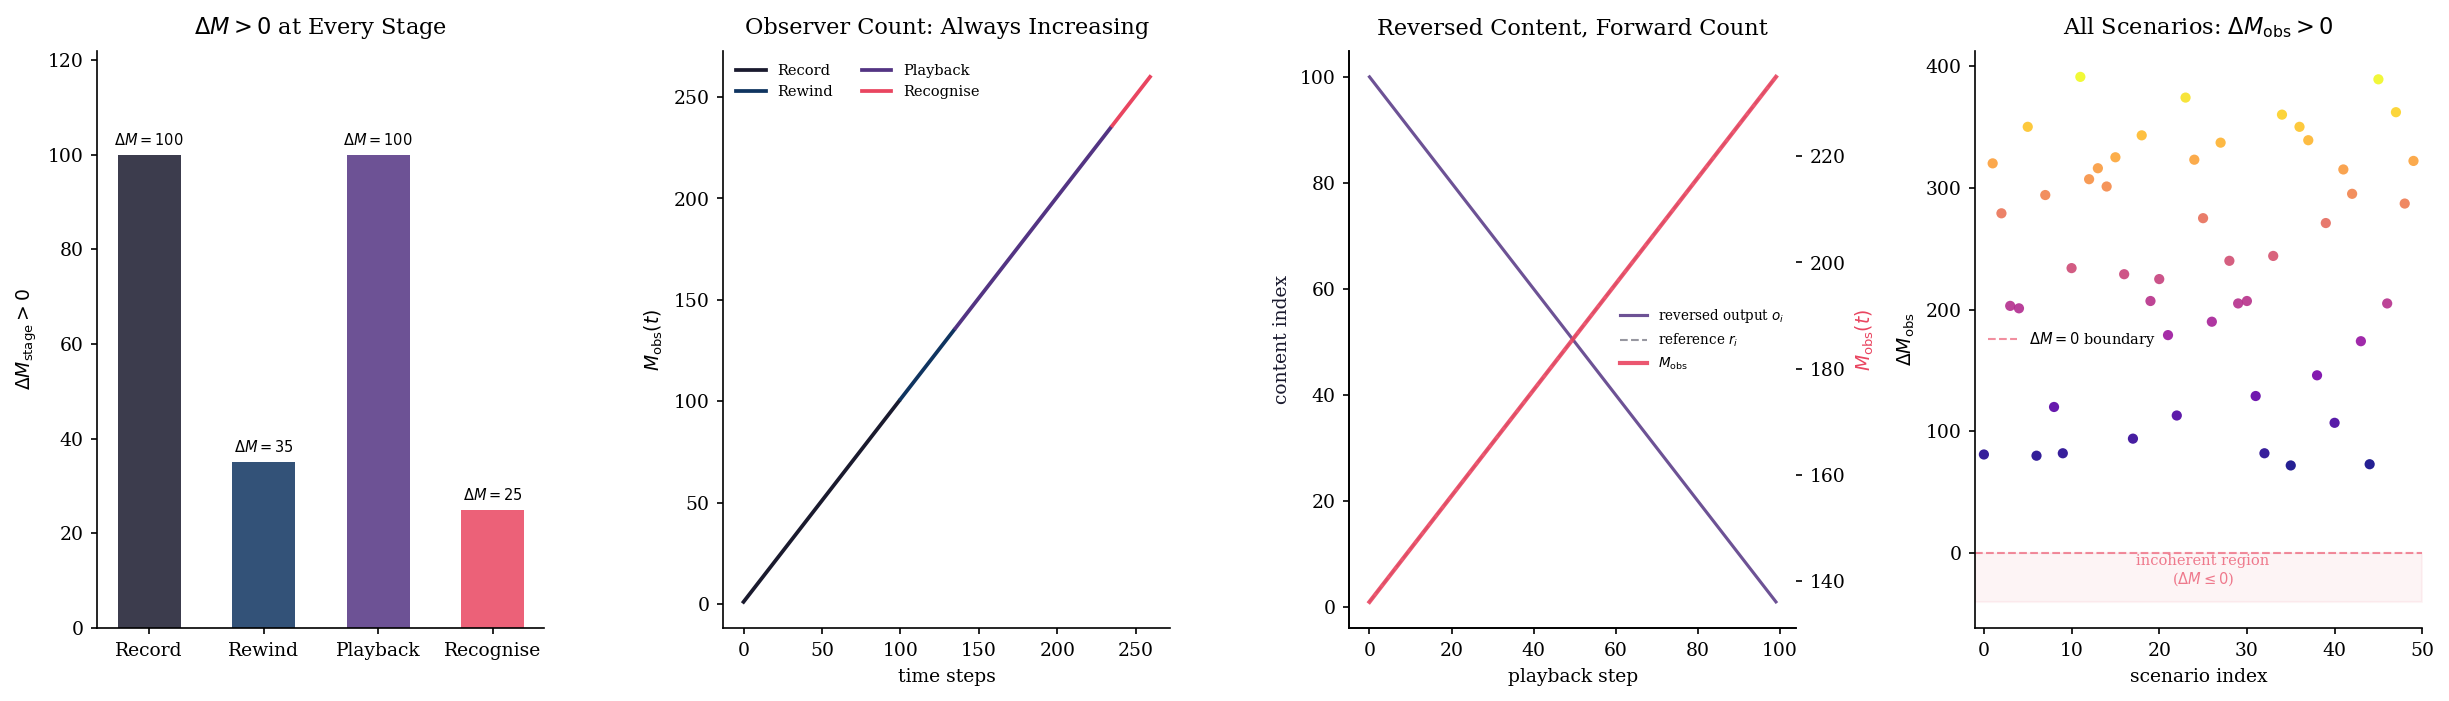
\includegraphics[width=\textwidth]{panels/panel_08_observer_forward_direction.png}
    \caption{\textbf{Every component of any apparent time-reversal scenario---production,
    mediation, and observation---is a forward partition event with $\Delta M > 0$;
    the temporal inversion is a property of output encoding, not of any partition count
    (Theorems~\ref{thm:forward-all} and~\ref{thm:obs-recognition};
    Remark~\ref{rem:cassette}).}
    (\textbf{A})~The cassette tape scenario decomposed into four stages (Record, Rewind,
    Playback, Recognise), with $\Delta M > 0$ annotated at each stage.  No stage has
    $\Delta M \leq 0$; the ``reversal'' lives entirely in the content-ordering of the
    output, not in the direction of any partition count.
    (\textbf{B})~The observer's cumulative count $M_{\mathrm{obs}}(t)$ across all four
    stages, coloured by stage.  The count is strictly monotone throughout: the observer
    advances forward in partition time during every phase of the observation, including
    the phase in which the reversed output is being perceived.
    (\textbf{C})~Reference sequence $\{r_i\}$ (dashed) and reversed output $\{o_i =
    r_{k+1-i}\}$ (solid) during playback (left axis), overlaid with
    $M_{\mathrm{obs}}(t)$ (right axis).  Content is in reverse order; the observer's
    partition count advances forward simultaneously.  The two axes are independent:
    content ordering and partition direction are separate predicates with no mutual
    implication.
    (\textbf{D})~For $50$ independent apparent-reversal scenarios, $\Delta M_{\mathrm{obs}} > 0$
    in every case, coloured by duration (plasma scale).  All points lie strictly above
    the $\Delta M = 0$ boundary (dashed); the incoherent region ($\Delta M \leq 0$)
    is shaded below.  No scenario witnesses or instantiates a backward partition event.}%
    \label{fig:panel8_observer_forward_direction}
\end{figure*}

% ──────────────────────────────────────────────────────────────────────────────
\begin{figure*}[!htbp]
    \centering
    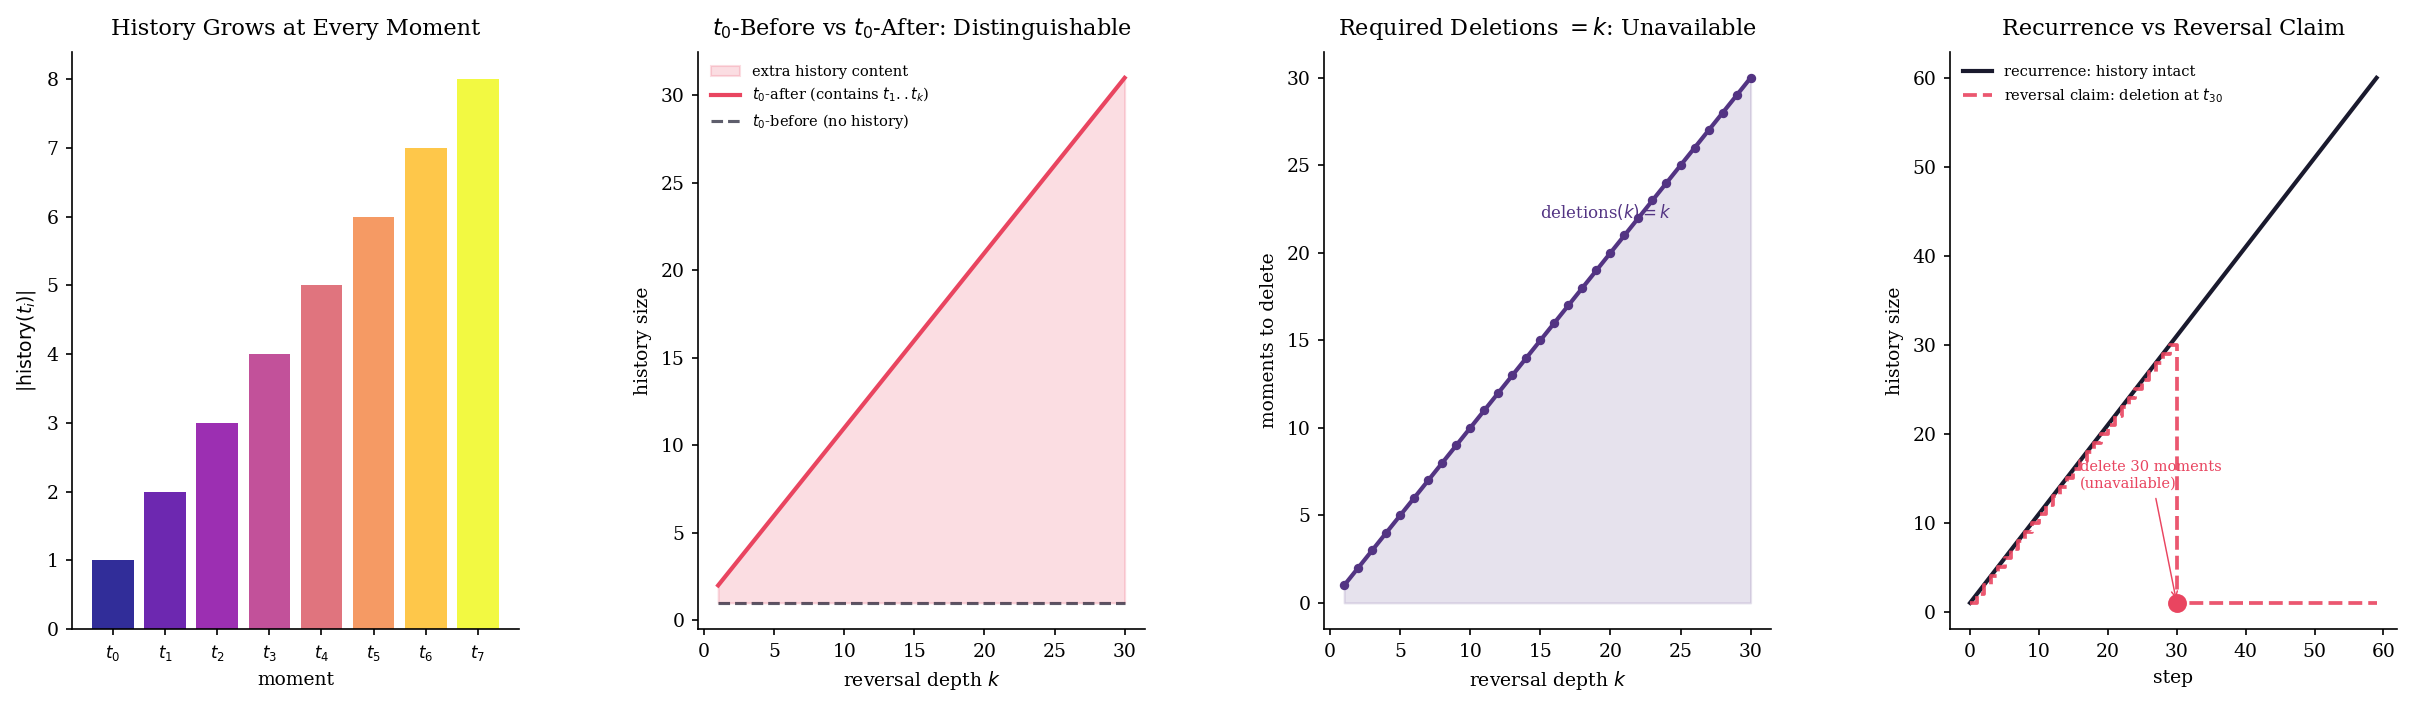
\includegraphics[width=\textwidth]{panels/panel_09_history_deletion.png}
    \caption{\textbf{Genuine time reversal from $t_k$ to $t_0$ requires deleting the
    intervening moments $t_1,\ldots,t_{k-1}$ from the universe's history; the required
    deletions grow linearly with reversal depth, and deletion is not an available
    physical operation
    (Theorems~\ref{thm:deletion} and~\ref{thm:no-deletion};
    Definition~\ref{def:distinguishability}).}
    (\textbf{A})~History size at each moment $t_i$: $|\mathrm{history}(t_i)| = i+1$,
    coloured by moment index (plasma scale).  History grows monotonically; no physical
    process reduces it.  The state at any moment includes the full causal record of all
    prior moments (Definition~\ref{def:distinguishability}).
    (\textbf{B})~State at $t_0$-before (history size $= 1$, dashed) versus state at
    $t_0$-after-reversal from depth $k$ (history size $= k+1$, solid), with shaded
    extra content.  The two states are distinguishable by their histories and are
    therefore distinct.  For the reversal claim to hold, the $k$ extra moments must be
    absent from the post-reversal state.
    (\textbf{C})~Required deletions as a function of reversal depth $k$:
    deletions$(k) = k$ exactly, growing linearly (shaded fill).  Any reversal of
    depth $k \geq 1$ requires at least one deletion; deletion is structurally
    unavailable (Theorem~\ref{thm:no-deletion}).
    (\textbf{D})~Recurrence (solid): history grows as the system evolves forward;
    at the recurrence step the configuration matches $t_0$ but the history is intact.
    Reversal claim (dashed): history would need to snap back to size $1$ at step $30$,
    requiring deletion of $30$ moments.  The sharp discontinuity marks the deletion
    event; no physical process produces it.  This panel directly visualises the
    distinction between recurrence and reversal established by
    Corollary~\ref{cor:egg-cycle}.}%
    \label{fig:panel9_history_deletion}
\end{figure*}

% ──────────────────────────────────────────────────────────────────────────────
\begin{figure*}[!htbp]
    \centering
    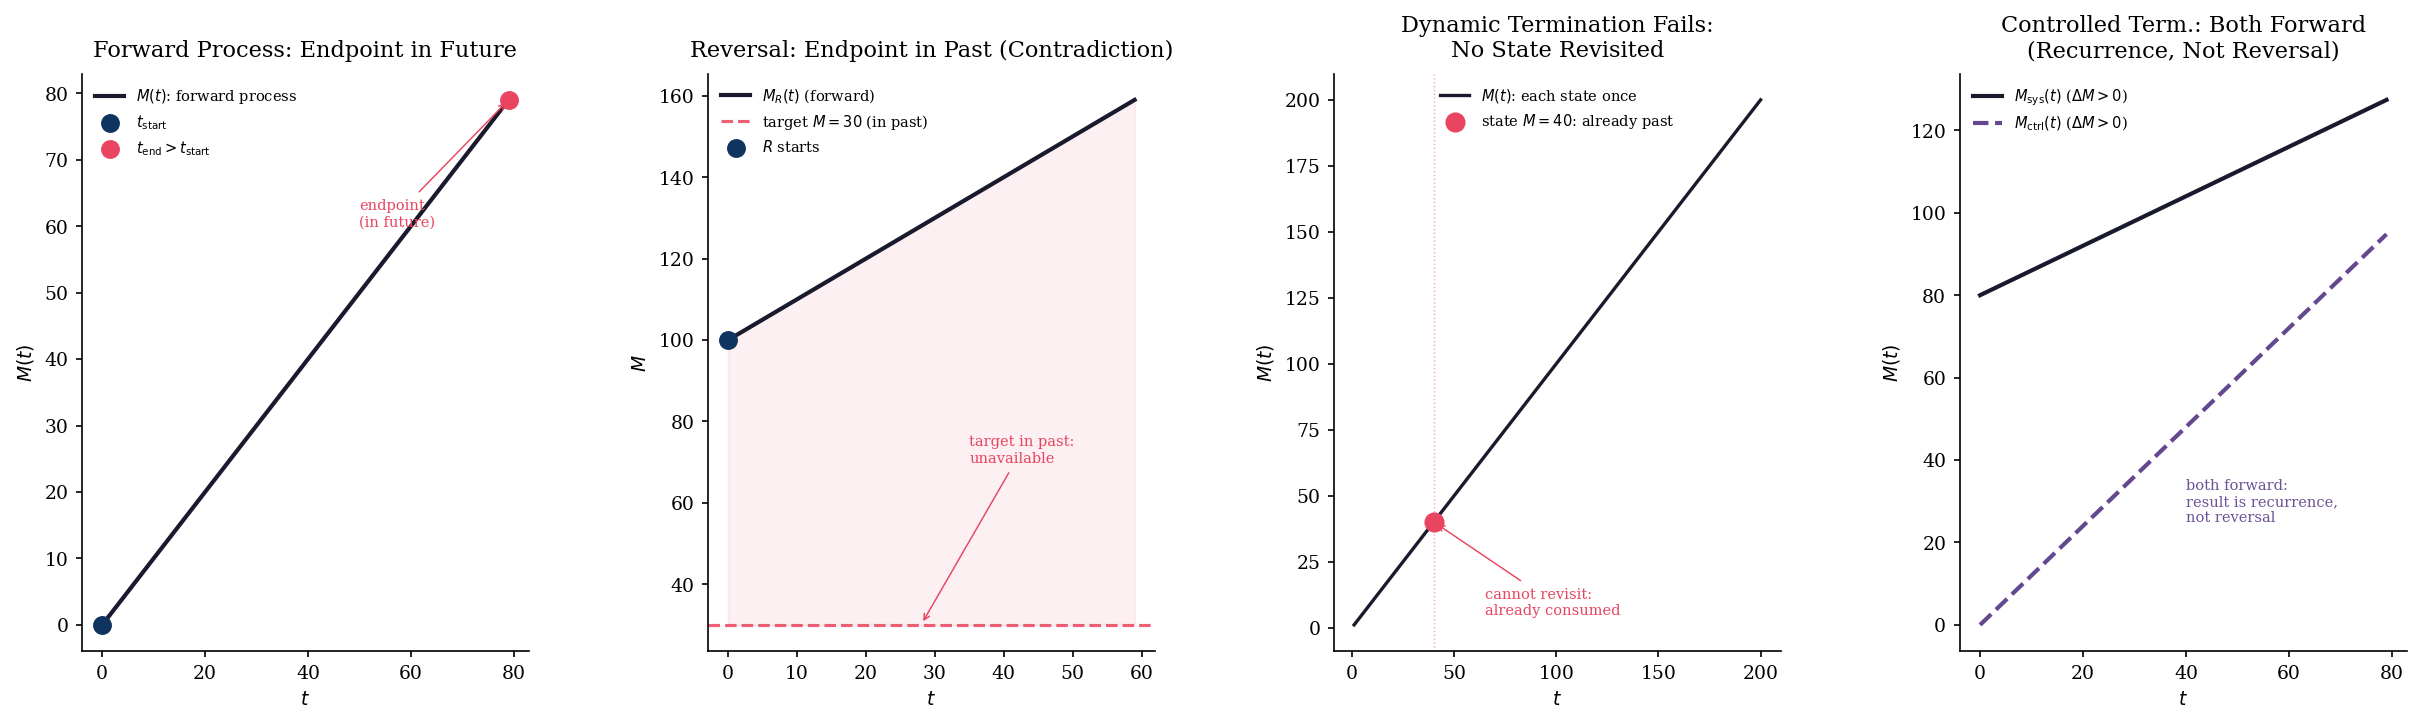
\includegraphics[width=\textwidth]{panels/panel_10_process_termination.png}
    \caption{\textbf{A reversal process $R$ has no available termination structure:
    its endpoint is a past state unreachable by dynamic termination
    (Corollary~\ref{cor:no-repeat}), and controlled termination collapses the reversal
    claim into a forward-time recurrence; no third mechanism exists
    (Theorem~\ref{thm:reversal-no-process}; Definition~\ref{def:process}).}
    (\textbf{A})~A forward process: $M(t)$ increases from $t_{\mathrm{start}}$ (blue) to
    $t_{\mathrm{end}}$ (orange).  The endpoint lies in the process's future; the
    forward dynamics determine when it is reached.  This is the canonical structure
    of any process in the sense of Definition~\ref{def:process}.
    (\textbf{B})~Putative reversal process $R$: $M_R(t)$ increases from $M = 100$ onward
    (forward time), but the target endpoint is the past state at $M = 30$ (dashed
    horizontal).  The gap between $M_R(t)$ and the target grows monotonically;
    dynamic termination cannot close this gap because the target recedes as $R$
    advances.
    (\textbf{C})~Dynamic termination fails: each partition state is visited exactly once
    along the forward trajectory (Corollary~\ref{cor:no-repeat}).  The state at
    $M = 40$ (orange marker) was consumed at step $40$ and cannot be revisited; a
    ``return'' requires a second visit, which the injectivity of $\Phi$ excludes.
    (\textbf{D})~Controlled termination yields recurrence, not reversal: both
    $M_{\mathrm{sys}}(t)$ (solid) and $M_{\mathrm{ctrl}}(t)$ (dashed) are strictly
    increasing.  The controller uses memory of a past configuration to navigate the
    system to a resembling configuration; both agents run forward.  This is a
    forward-time memory-driven recurrence of the kind formalised in
    Corollary~\ref{cor:egg-cycle}, not genuine reversal.}%
    \label{fig:panel10_process_termination}
\end{figure*}
